\documentclass[12pt,a4paper]{book}

\usepackage [english]{babel}
\usepackage [utf8]{inputenc}

%\usepackage[left=2.5cm,right=2.5cm,top=2.5cm,bottom=2.5cm]{geometry}

\usepackage{longtable}
 
%\setcounter{secnumdepth}{3} % le estoy indicando la profundidad hasta donde tiene que mostrar en el indice
%\setcounter{tocdepth}{4} 

\usepackage[titletoc]{appendix}

\RequirePackage[paperwidth=17cm,paperheight=24cm,inner=15mm,outer=20mm,top=25mm,bottom=25mm]{geometry} %%dimensiones externas del pdf y margenes internos.

\usepackage [T1]{fontenc}
\usepackage{graphicx}
\usepackage{graphics}
\graphicspath{ {Figures/} } %Para buscar las imágenes en otra carpeta
\usepackage{amsfonts} %Para poder escribir letras como la matriz identidad
\usepackage{mathrsfs} %Para poder escribir letras como la H del el espacio de Hilbert
\usepackage{slashed} % para la barra cruzada
\usepackage{amsmath}
\usepackage{amssymb}
\usepackage{makeidx}
\usepackage{hepunits} %para poder utilizar unidades
\usepackage[version=3]{mhchem} %para poder escribir los simpolos atómicos y químicos
%\usepackage{hep}

%\renewcommand{\figurename}{ Figura}
%\usepackage[labelsep=endash]{caption}

%\usepackage[figurename=\bold{Figura}]{caption}
%\usepackage [labelformat=empty]{caption}
%\usepackage{wrapfig} %for I can use wrapfigure
\usepackage[font={small, up}]{caption}
\usepackage[caption = false]{subfig} %% for putting several pictures in the same line
\usepackage{hyperref} %hipervinculos del índice
\setlength{\parindent}{4em} %para que interprete la linea en blanco como un \parragraph{}
\setlength{\parskip}{1em}
%\usepackage{subcaption}
%\usepackage[caption = false]{subfig}


\renewcommand{\baselinestretch}{1.15}
%\renewcommand{\thefigure}{}

%para aumentar el espacio entre elementos del índice
\usepackage{setspace}

\bibliographystyle{unsrthep}



\begin{document}
\captionsetup[figure]{labelfont={bf},labelformat={default},labelsep= endash,name={Figura}}
\begin{titlepage}

\begin{center}
%\vspace*{-1 cm}
%\vspace*{1 cm}
%%\begin{figure}[htb]
%%\begin{center}
%%
\includegraphics[scale=0.7]{1Cover_page/Logo1.png}
%%\end{center}
%%\end{figure}
%%\vspace*{0.2 cm}


%\vspace*{0.2in}
{\large Facultad de Física}\\
{\large Departamento de Fisica Atómica, Molecular y Nuclear}\\
\vspace*{0.2in}
\vspace*{0.6in}
\end{center}
\vspace*{-1in}
\begin{center}
\vspace*{1 cm}


\begin{figure}[htb]
\begin{center}

\includegraphics[scale=0.06]{1Cover_page/Logo2.jpg} 
\end{center}
\end{figure}
\vspace*{1 cm}

\begin{large}
%%\textbf{{\large Thesis}}\\
%%\rule{80mm}{0.1mm}\\
%\vspace*{2 cm}

\end{large}
%%\vspace*{0.2 cm}
\begin{Large}
\textbf{\LARGE TRITIUM: Design, construction and commissioning of an in-water tritium detector} \\
\end{Large}
%\vspace*{0.3in}
\vspace*{1.2 cm}

\begin{large}
\textbf{Marcos Martínez Roig}\\
PhD in Physics\\
\today
\end{large}
\end{center}

\vspace*{-1.2 cm}
%\rule{80mm}{0.1mm}\\
%\vspace*{0.1in}
\begin{large}
\begin{flushright}
\item[\bf Under the supervison of:]\quad  \\ 
José Díaz Medina\\
Nadia Yahlali Haddou\\
\end{flushright}
\end{large}

\end{titlepage}


$\ $
\thispagestyle{empty}  % para que no se numere esta pagina
\chapter*{}

\pagenumbering{Roman} %for using romain numbers (page numering)


\begin{flushright}
\textit{Dedicated to \\
my family}
\end{flushright} 

\newpage

\chapter*{Acknowledgements} \label{chap:Acknowledgements}  %pongo el asterisco para que no se numere ni aparezca en el índice
%%\cleardoublepage
\addcontentsline{toc}{chapter}{Acknowledgements} % para que aparezca en el indice de contenidos
AGRADECER A: PEPE, NADIA, MIREIA, ANA, MARQUITOS, ANDREA, COMPAÑEROS DE DESPACHO Y DEL IFIC/UV (NOMBRAR TODOS), GENTE DEL LARAM (TERESA, VANESA, ROSA, CLODO), ANSELMO Y MIGUEL, INGENIEROS DE NEXT, GENTE DE PORTUGAL, Antonio de extremadura, gente de francia... Y PENSAR GENTE QUE ME DEJO POR EL CAMINO. A DAVID CALVO DEL IFIC, A DAVID CANAL DE SAMTEC, A LUIS FERR... DE PETSYS... A LIDON DEL ICMOL... Ana Ros, Jhon Barrio y Gabriela Llosa del IFIMED. Al programa interreg sudoe -> Soporte financiero!

\newpage

\chapter*{Abstract} \label{chap:Abstract}
%%\cleardoublepage
\addcontentsline{toc}{chapter}{Abstract} % para que aparezca en el indice de contenidos
%LEER LOS 2 ABSTRACS DE ANA MAS LOS ABSTRACS QUE TENGO YO DE LAS CONFERENCIAS Y ARTICULOS (ARTICULOS ALEATORIOS MAS EL DE CARLOS, EL MIO, EL DE NADIA, ETC)

%\begin{abstract}
%Texto           del           abstract
%\end{abstract}

\newpage


\chapter*{Nomenclature and acronyms} \label{chap:NomenclatureAcronyms}  %pongo el asterisco para que no se numere ni aparezca en el índice
%%\cleardoublepage
\addcontentsline{toc}{chapter}{Nomenclature and acronyms} % para que aparezca en el indice de contenidos
\begin{longtable}{p{25mm} c p{120mm} }
\multicolumn{3}{l}{Acronyms:}\\
\\
$OECD$ & --- & Organisation for Economic Co-operation and Development\\
$Btu$ & --- & British termal unit\\
$UN$ & --- & United Nations\\
$UNFCCC$ & --- & United Nations framework convention on Climate change\\
$ITER$ & --- & International Thermonuclear Experimental Reactor\\
$NPP$ & --- & Nuclear Power Plants\\
$DOE$ & --- & Department of Energy\\
$U.S.A.$ & --- & United States of America\\
$U.S.$ & --- & United States\\
$EPA$ & --- & Environmental Protection Agency\\
$LDL$ & --- & Lower Detection Limit\\
$PWR$ & --- & Pressurized Water Reactor\\
$BWR$ & --- & Boiled Water Reactor\\
$PHWR$ & --- & Pressurized Heavy Water Reactor\\
$quasi-real$ & --- & Less than 10 minuts\\
$LSC$ & --- & Liquid Scintillation Counting\\
%$IUPAC$ & --- & International Union of Pure and Applied Chemistry\\
$LWR$ & --- & Liquid Water Reactor\\
$STP$ & --- & Standard temperature ($0\celsius$) and pressure ($1$ atm)\\
$IC$ & --- & Ionization chamber\\
$BIXS$ & --- & Beta Induced X-ray Spectrometry\\
$PMT$ & --- & PhotoMultiplier Tube\\
$SDD$ & --- & Silicon Drift Detector\\
$EEC$ & --- & European Economical Community\\
$SiPM$ & --- & Silicon PhotoMultiplier\\
$ALARA$ & --- & As Low As Reasonably Achievable\\






$T$ & --- & Temperature (ºC).\\
$V$ & --- & Volume (m$^3$).\\


\\
\\
\multicolumn{3}{l}{Atomic and nuclear symbols}\\
\\
$\ce{CO_2}$ & --- & Carbon Dioxide\\
$\ce{CH_4}$ & --- & Methane\\
$\ce{N_2 O}$ & --- & Nitrous oxide\\
$\ce{HFC}$ & --- & Hydrofluorocarbons\\
$\ce{PFC}$ & --- & Perfluorocarbons\\
$\ce{SF_6}$ & --- & Sulfur Hexafluoride\\
$\ce{^{1}_{1}H}$ & --- & Hydrogen\\
$\ce{^{2}_{1}H}$ & --- & Deuterium (Non-radiactive hydrogen isotope, 1 neutron)\\
$\ce{^{3}_{1}H}$ & --- & Tritium (radiactive hydrogen isotope, 2 neutrons)\\
$\ce{^{4}_{2}He}$ & --- & Helium\\
$\ce{^{3}_{2}He}$ & --- & Isotope of the Helium(Non-radiactive, 1 neutrons)\\
$\ce{n}$ & --- & free neutron\\
$\becquerel$ & --- & Becquerel, Nuclear decay number per second\\
$\liter$ & --- & Liter\\
$\becquerel/\liter$ & --- & Becquerel per liter\\
$Ci$ & --- & Curios\\
$Ci/L$ & --- & Curios por litro\\
$yr$ & --- & year\\
$\giga\watt$ & --- & Giga watt\\
$T_{1/2}$ & --- & Half-life time of a radioactive element\\
$\beta$ & --- & Beta decay\\
$\ce{\overline{\nu}_e}$ & --- & Electron antineutrino\\
$\ce{e^-}$ & --- & Electron\\



$\gamma$ & --- & Gamma decay\\
$\alpha$ & --- & Alpha decay\\
\\
\\
\multicolumn{3}{l}{Añadir en un futuro:}\\
\\
D\&D & --- & Decontamination and Decommissioning.\\
DWS & --- & Drinking water standars\\
UDL & --- & Upper Detection Limit\\


NA & --- & Numerical Apertures\\
PMMA & --- & Polymethyl Methacrylates\\
UV & --- & ULtraviolet\\
WLS & --- & Wavelength shifter\\
\end{longtable}


%%añadir bibliografía al indice
\let\OLDthebibliography=\thebibliography
\def\thebibliography#1{\OLDthebibliography{#1}%
\addcontentsline{toc}{chapter}{\bibname}}

%%indice
\tableofcontents

\cleardoublepage
\addcontentsline{toc}{chapter}{Lista de figuras} % para que aparezca en el indice de contenidos

%%lista de figuras
\listoffigures

\cleardoublepage
\addcontentsline{toc}{chapter}{Lista de tablas} % para que aparezca en el indice de contenidos

%%lista de tablas
\listoftables

%%%%%%%%%%%%%%%%%%%%%%%%%%%%%%% MAIN BODY %%%%%%%%%%%%%%%



\chapter{Introduction}  \label{chap:GeneralIntroduction} %(%(I have to use latin numbers inside of this chapter))
\pagenumbering{arabic} %for using romain numbers (page numering)
%%\setcounter{page}{-1} %%first number of the counter
	\section{Global energy context}
	The energy necessities around the world has been increased a $60\%$ in the last 25 years and they are growing each day due to, mainly, the strong population growth (mundial population has been increased in a $40\%$ between $1990$ and $2015$) and the fast development of emerging countries like China, India and Brazil. \cite{Renovables}. 

On top of that the outlook is that it will keep increasing as you can see in the figure \ref{fig:Wolrd_energy_consumption_a}, specially for countries which don't belong to the OECD like countries which I have said before. In this figure you can see that the energy quantity which will be used on 2040 is expected to be the double of the one which we used in 2000. 

Nowadays, as you can see in the figure \ref{fig:Wolrd_energy_consumption_b}, the most used elements for getting the energy that we use are liquid fuels, coal and natural gas, namely, natural elements. This fact has two problems. On the one hand, natural elements are limitated and this is a problem due to the huge increasing of the energy consumed in the world and, on the other hand, obtaining energy from these natural elements produces large amounts of greenhouses gases (mainlty $CO_2$) which contribute to the environmental contamination, global warming, deforestation, etc. and this is a very big problem, specially right now, since United Nations (UN) did a communication on November 25, 2019 \cite{HighestCO2}, where they claimed that the lifestyle of the world population has not changed in the last years and, as a reason of that, we achieved the highest level of the \ce{CO_2}.

\begin{figure}[]
 \centering
  \subfloat[]{
    \label{fig:Wolrd_energy_consumption_a}
    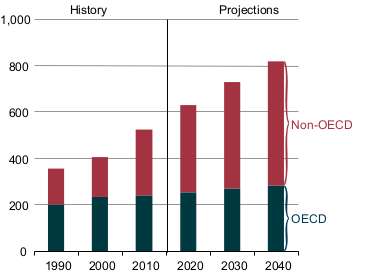
\includegraphics[width=0.5\textwidth]{2Introduction/world_energy_consumption_bar.png}}
  \subfloat[]{
    \label{fig:Wolrd_energy_consumption_b}
    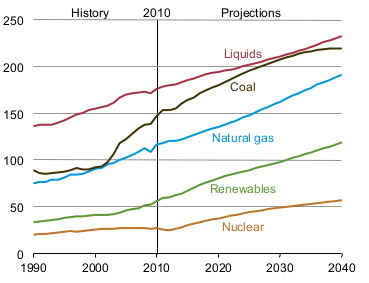
\includegraphics[width=0.5\textwidth]{2Introduction/world_energy_consumption_graph.png}}
 \caption{World energy consumption from 1990 up to now and outlooks for the future until $2040$ (units in $10^{15}~Btu$) \cite{EIA}}
 \label{fig:Wolrd_energy_consumption} 
\end{figure}

In order to control these emissions, the United Nations in the Framework Convention about Climate Change (UNFCCC), has developed a protocol, whose name is Kyoto \cite{Kyoto}. The objective of this protocol is to control and reduce the global negative envirionmental impact. It is focused on 6 different gases, carbon dioxide ($\ce{CO_2}$), methane ($\ce{CH_4}$), nitrous oxide ($\ce{N_2 O}$) and other three types of fluorinate industrial gases ($\ce{HFCs}$, $\ce{PFCs}$ and $\ce{SF6}$), which are related with the greenhouse effect and whose consecuence is the global warming. This convention only encourage to belonging countries to the United Nations to reduce their greenhouses gases emissions but this protocol commits the countries who has signed it to do so.

Therefore, we currently have a problem because, on the one hand, we want to maintain, even increase, this economic growth and for that we need to produce as much energy as we can but, on the other hand, we need to reduce the negative environmental impact. Hence, what we need is a energy source with which we can get a big quantity of energy with a very low greenhouse gases emisions. One possibility which we have is the nuclear fusion plants. They don't emit greenhouse gases and with its energy, which is practically limitless, we could satisfy the humanity's energy necesities .

The largest representative in this sector is the ITER \cite{ITER} (International Thermonuclear Experimental Reactor) that is going to be the largest fusion reactor in the world. The ITER is currently under construction in Cadarache, France, and its objective is to provide the concept of sustained fusion. The reaction which ITER try to reproduce in the earth is the fusion reactor using deuterium ($\ce{^{2}_{1}H}$) and/or tritium ($\ce{^{3}_{1}H}$) because it is the only one whose requirements of temperature (several hundreds of millions degrees) and pressure we can fulfill in the earth. Among the possible combinations between both (table \ref{tab:FusionReactions}), the choice of ITER is the nuclear reaction between deuterium and tritium in a 50:50 mixture because, as you can see in this table,  it is the nuclear reaction with which we get the highest energy release. 

\begin{table}[htbp]
%%\centering
\begin{center}
\begin{tabular}{|c|c|c|}
\hline
Reaction & Products & Energy gain ($\MeV$) \\
\hline \hline \hline
$\ce{^{2}H}+\ce{^{3}H}$ & $\ce{^{4}He}+\ce{n}$ & $17.6$ \\ \hline
$\ce{^{3}H}+\ce{^{3}H}$ & $\ce{^{4}He}+2\ce{n}$ & $11.3$ \\ \hline
$\ce{^{2}H}+\ce{^{2}H}$ & $\ce{^{3}H}+\ce{^{1}H}$ & $3.98$ \\ \hline
$\ce{^{2}H}+\ce{^{2}H}$ & $\ce{^{3}He}+\ce{n}$ & $3.25$ \\ \hline
\end{tabular}
\caption{Fusion reactions between deuterium and tritium\cite{TritiumDocument}}
\label{tab:FusionReactions}
\end{center}
\end{table}

Nevertheles, the fusion power plants is not already prepared for working,  they are still in experimental phase and its researchers need to solve some important problems like inestabilitiy vortex, materials which withstand such high temperatures, etc. \cite{FusionCourse}. Hence, although we know that the future nuclear fusion plants will be the energy of the future, nowadays, we have to wait until all their problems has been resolved.

Other possible  energy source is the existing Nuclear Power Plants (NPPs). With the NPPs we can practically avoid the problem of the greenhouse gases emission. We have to take into account that, although the nuclear fission reaction doesn't emit greenhouse gasses, the total procces to obtain the energy, which involves the uranium mining and milling, transport, uranium enrichment, etc., has a small contribution to the annual release of greenhouses gases. These emissions are difficult to estimate because, on the one hand, they depend on the NPP that we consider (for instance, there are studies which show that asian NPPs has higher emissions \cite{ComparationEmissions}) and, on the other hand, there are some tasks whose greenhouse gases emission are difficult to quantify\cite{ComparationEmissions}. 

There's exist a study \cite{ComparationEmissions} which analyzes $19$ different studies of different NPPs. His estimation for the total greenhouses gases emision of a NPP is $66~\gram~CO_2 /\kilo\watt\hour$ which was obtained as a average of these $19$ studies considered. In the table \ref{tab:ComparationEmisions} this estimation is compared with the estimation for other energy kinds. There you can check that, the emissions due to NPPs is much more smaller, one order or more, than the emissions from burning natural elements.

\begin{table}[htbp]
%%\centering
\begin{center}
\begin{tabular}{|c|c|}
\hline
Technology & Estimate ($\gram~CO_2 /\kilo\watt\hour$)\\
\hline \hline
Wind & $9-10$ \\ \hline
Hydroelectric & $10-13$ \\ \hline
Biogas & $11$ \\ \hline
Solar thermal & $13$ \\ \hline
Biomass & $14-41$ \\ \hline
Solar PV & $32$ \\ \hline
Geothermal & $38$ \\ \hline
Nuclear & $66$ \\ \hline
Natural gas & $443$ \\ \hline
Fuel cell & $664$ \\ \hline
Diesel & $778$ \\ \hline
Heavy oil & $778$ \\ \hline
Coal & $960-1050$ \\ \hline
\end{tabular}
\caption{Estimations of $\ce{CO_2}$ emissions for several kinds of energy sources\cite{ComparationEmissions}}
\label{tab:ComparationEmisions}
\end{center}
\end{table}

NPPs are already working and, nowadays, they are essential for providing a big part of the electic power that is used in the current world (more than a 20\% in Spain as you can see in the table \ref{tab:PercentageEnergySpain}). 

\begin{table}[htbp]
%%\centering
\begin{center}
\begin{tabular}{|c|c|c|c|}
\hline
Type of energy source & Contr. & Type of energy source & Contr.  \\
\hline \hline
Nuclear & $22.0\%$ & Wind & $20.9\%$  \\ \hline
Coal & $4.2\%$ & Hydraulics & $9.7\%$  \\ \hline
Combined Cycle & $20.1\%$ & Solar Photovoltaic & $3.5\%$  \\ \hline
Cogeneration & $11.8\%$ & Solar thermal & $2.0\%$  \\ \hline
No-renewable waste & $0.8\%$ & Other renewables & $1.4\%$  \\ \hline
Pumping turbine & $0.6\%$ & renewable waste & $0.3\%$  \\ \hline
 &  & \parbox{11em}{\centering Impoted balance of\\  international exchanges} & $2.7\%$\\ \hline
\end{tabular}
\caption{Contribution of each energy source to the total energy consumed in Spain in 2019 \cite{PercentageEnergySpain}}
\label{tab:PercentageEnergySpain}
\end{center}
\end{table}

NPP is one of the cheapest source. It is a stable source which doesn't depend on  meteorological parameters and, although there are other alternative energy sources which are being developed quickly  (photovoltaic, wind, tidal energy, etc.), even other concepts of energy production and saving (local production, solar roofs, energy efficiency, smart cities, etc.), today they are not develop enough.  

The detractors of nuclear energy argue that NPPs facilitate nuclear proliferation or there are a risk of radiactive contamination and accidents like it happened in the past: Chernobyl, Fukushima and other accidents with lesser impact such as Three Mile Island, near to Pensilvania, USA.

Although we know that the nuclear energy is not the energy of the future since it produces nuclear waste which, by the moment, we don't know how we can eliminate, it is difficult that we leave to use nuclear energy because, now, we don't have a better solution for obtaining the energy which we need. 

In Spain the government are doing an effort in order to remove all nuclear power plants. This is because they are not going to build new nuclear reactors and they are only waiting until the NPPs have reached the end of their useful life (approximately 40 years). They expect to close all NPPs between $2020$ and $2030$ \cite{CloseNPP}. 

Other countries like France, where the $77\%$ of their energy consumed is obtained from nuclear sources, prefer to maintain their nuclear facilities and there's even exist other countries that believe that nuclear energy is a safe investment like China who announced in 2016 that they were going to build 60 new nuclear reactors in the next dedade \cite{60ReactorsChina} or USA, who made an investment of 35 million of euros in 2019 for development and improvement of nuclear power plants \cite{35MillionsUSA}. 

In any case it is not important if we agree or not with nuclear energy source. The only important thing is that the nuclear energy production in the world is not going to stop in the next decade, in fact, it will increase as you have seen in the outlooks of the figure \ref{fig:Wolrd_energy_consumption_b}. Therefore the development of  different types of alarm systems is a good investment of both, time and money. Safety is not a negotiable aspect and there must be mechanisms that warn us of any malfunction of a nuclear power plant. Hence, our work has based on the development of a monitor that we can use as early alarm in case of any problem happen in a NPP.

Generally, a nuclear reactor, which is working in normal mode, is characterized by extreme stability and, therefore, by a constant emission of radioactive isotopes so the first alarm signs of any malfunctioning of a NPP is a variation of this radiactive emission rate.

Between all the radioactive elements which is produced in a nuclear power plant, the most frequently produced is tritium as DOE complex \cite{FiberDetector1a} \cite{FiberDetector1b}  and other research facilities in China \cite{CommonEmissionTritium} have seen in their installations and in ground water, surface water, and process waste water around their facilities. However, as we will see in the section \ref{sec:StateOfTheArt}, the current methods which is used for monitoring this radioactive element has some limitations. 

Therefore, the radiactive element which we have chosen for monitoring with our early alarm system is tritium. We have focused our alarm system for working with NPPs but it could be also interesting for other tasks where tritium is involved like monitoring the behaviour of future fusion nuclear plants (ITER will need up to several tens of kilograms of tritium for working, which correspond to several $\tera\becquerel$ of tritium.) or any nuclear research facility (tritium is a commun emission of these places \cite{FERMILAB},\cite{BrookHavenNationalLaboratory}),  tracking the movement of tritium contaminated plumes in ground water \cite{TrackingTritium} or demonstrate the compliance with the government agencies which fix the limit of the emitted radionuclides to the environmental. 

We have to take into account that the limit of the emission of each radioactive element depends on the government agency who manages it, and the regulation directives that is implemented in that place so, as a consequence, it is different in each country. For example, in Europe, the agency is Council Directive and the limit which they have stablished for tritium in drinking water is $A = 100~\becquerel/\liter$ \cite{100BqL}. In USA, the organization is United States Envirnomental Protection Agency (U. S. EPA) and this limit is $A = 20~\nano\curie/\liter = 740~\becquerel/\liter$ \cite{740BqL}.

Tritium is normally produced in the water that there are in the cooling system or the moderator of some NPPs. It usually appear by neutron capture of the deuterium, which exist in the heavy water ($D_2 O$), semi-heavy water ($H D O$) or the deuterium which has created by neutron capture in usual water ($H_2 O$). All these processes have a big probability to happen due to the huge quantity of neutrons which we has in the nuclear reactor, $10^{14} ~\ce{n} \, \cm^{-2} \second^{-1}$ \cite{CrossSeccionNeutrons}. 

The quantity of tritium will be different for each reactor type because, as we will see in the next seccion, the cross section of tritium production will depend on the materials which there are in any type of NPP. In the table \ref{tab:TritiumEmisionsNPPs} we can see the emissions of different types of nuclear reactors:

\begin{table}[htbp]
%%\centering
\begin{center}
\begin{tabular}{|c|c|c|}
\hline
Reactor type & Gaseous discharge ($\giga\becquerel/$y) & Liquid discharge ($\giga\becquerel/$y) \\
\hline \hline \hline
PWR & $3.70\cdot 10^{3}$ & $2.59\cdot 10^{4}$ \\ \hline
BWR & $1.85\cdot 10^{3}$ & $3.70\cdot 10^{3}$ \\ \hline
HWR & $7.40\cdot 10^{5}$ & $1.85\cdot 10^{5}$ \\ \hline
GCR & $7.40\cdot 10^{3}$ & $1.11\cdot 10^{4}$ \\ \hline
\end{tabular}
\caption{Emission of tritium in several different types of nuclear reactors\cite{CommonEmissionTritium}}
\label{tab:TritiumEmisionsNPPs}
\end{center}
\end{table} 

The tritium which is created in the water of the cooling system is finally released partially or totally to the environment. Between these types, the most common way is $\ce{HTO}$ \cite{CommonEmissionTritium}.

Our alarm system will monitor the activity of tritium in the water of the cooling system of the NPP which is emitted to the environmental. It can also work for the water of the moderator in these types of NPP but it's not our objective because it's a close circuit so it's not a emission (unless the moderator is leaking, in which case our alarm system would detect it indirectly due to a variation of tritium activity in the water of the cooling system released to the environment).

The measurement of the tritium activity is one of the systematic environmental control which is performed during energy production by NPPs. It is normally done by LSC technic which has a very good detection capability and precision but it has some problems, for example, it needs too long time for taking a measurement (2 days or more). I will speak more about LSC technic in the section \ref{sec:StateOfTheArt}.

The detection of this tritium in quasi-real time ($<10~\min$) is important because of the following reasons:

\begin{enumerate}

\item{} It can warn us about the production of an excesive number of neutrons in the nuclear reactor due to the overheating of itself or a leakage of the water from the primary circuit of the cooling system in a nuclear power plant due to some break (perhaps because of an excesive preassure, other alarm sign of a malfunctioning of a nuclear reactor). Both causes could become in a very dangerous problems so the tritium detection in quasi-real time could be important in order to quickly detect and to solve it.

\item{} This water, which there are in the secondary circuit of the cooling system, will be released to the eviromental, usually rivers or seas, after using it for cooling purposes. Generally this water will be used for human consuming, irrigation of all kind of plantations or it will arrive to a places where we fish. 

Due to such a low legal limit in comparation with the activities of tritium inside of a nuclear reactor, it is possible that, if the nuclear power plant don't work correctly, the activity of tritium water released will overcome this limit and it become this water in no drinkable and these crops into inedibles. On top of that, the life time of tritium is more than 12 years so these places will remain contaminated during a lot of time. 

\item{} There's exist a lot of rivers or seas, which is used for cooling systems of the nuclear power plants, that are crossborders, that's, they are shared by several countries like our case as we will see in the seccion \ref{sec:TritiumProject}. The emisión of an excessive tritium activity of one country could be affect severely to the other country creating new international conflicts between them.

\end{enumerate}

Because of all these reasons it is very important that we have an alarm system which is capable of measuring such low tritium activities in quasi-real time. Nevertheless, as we will see in the section \ref{sec:StateOfTheArt}, currently there are not any technic with which we can fulfill these requeriments.

All these reasons has motivated the project \textit{Tritium}, whose objective is the development of a system for quasi-real time monitoring of low radioactive levels of tritium in water for security applications in nuclear power plants. \label{sec:Introduction}
	\newpage

	\section{Tritium properties}
	Tritium is the only radioactive isotope of hydrogen. It was first time produced in $1934$ from neutron capture of deuterium by Ernest Rutherford, Mark Oliphant and Paul Harteck \cite{TritiumDiscovery} and it was first time isolated in 1939 by Luis Walter Alvarez and Robert Cornog \cite{TritiumIsolate}, who checked that tritium is a radiactive element. 

Tritium can be found in the environment since it is normally produced through the interaction of cosmics rays and gaseous elements of the upper atmosphere like nitrogen ($\ce{^{14}N}(\ce{n},\ce{^{3}H})\ce{^{12}C}$) \cite{TritiumHandling} and oxigen ($\ce{^{16}O}(\ce{n},\ce{^{3}H})\ce{^{14}N}$) \cite{OxigenTritium}. Then tritium becomes water (\ce{HTO}) and reaches the earth's surface as rain with an estimated produccion rate of $4\cdot 10^6 ~\curie/$yr \newline ($1.48 \cdot 10^8 ~\giga\becquerel/$yr) \cite{CommonEmissionTritium} \cite{TritiumHandling} . 

Tritium can be produced artificially in the environment from many different anthropogenic origins. There are a big amount of tritium which was produced on militar nuclear test explosions between 1945 and 1975, whose estimed produccion rate is $8 \cdot 10^9~\curie$ ($2.96 \cdot 10^11~\giga\becquerel$) and a part of that still remain. It was mainly produced from the nuclear reactions $\ce{^{14}N}(\ce{n},\ce{^{3}H})\ce{^{12}C}$ and $\ce{^{2}H}(\ce{n},\gamma)\ce{^{3}H}$. Tritium can be also produced by commercial producers of radioluminicent and neutron generator devices ($1 \cdot 10^6$ $~\curie/$yr), nuclear power and defense industries (less than $2 \cdot 10^6~\curie/$yr), several research facilities and nuclear reactor operation ($2 \cdot 10^6 \curie/\giga\watt$yr), whose main production channels are \cite{CommonEmissionTritium} \cite{TritiumHandling}:

\begin{equation}
\ce{^{2}_{1}H}(\ce{n},\gamma)\ce{^{3}_{1}H} \qquad \sigma_{th}= 5.2 \cdot{} 10^{-4}~\barn  ~~~\cite{CommonEmissionTritium}
\label{capneuH2}
\end{equation}

\begin{equation}
\ce{^{3}_{2}He}(\ce{n},\ce{p})\ce{^{3}_{1}H} \qquad \sigma_{th}= 5330~\barn ~~~\cite{CommonEmissionTritium}
\label{capneuHe3}
\end{equation}

\begin{equation}
\ce{^{6}_{3}Li}(\ce{n},\alpha)\ce{^{3}_{1}H} \qquad \sigma_{th}= 940~\barn ~~~\cite{CommonEmissionTritium}
\label{capneuLi6}
\end{equation}

%%\begin{equation}
%%\ce{^{7}_{3}Li}(\ce{n},\alpha)\ce{^{3}_{1}He} + \ce{n} ~~~\cite{CommonEmissionTritium}
%%\label{capneuLi7}
%%\end{equation}

\begin{equation}
\ce{^{10}_{5}B}(\ce{n},2\alpha)\ce{^{3}_{1}H} \qquad \sigma_{th}= 3835~\barn ~~~\cite{CommonEmissionTritium}
\label{capneuB10}
\end{equation}

%\begin{equation}
%\ce{^{11}_{5}B}(\ce{n},2\alpha)\ce{^{3}_{1}H} + n ~~~\cite{CommonEmissionTritium}
%\label{capneuB11}
%\end{equation}
%$\eqref{capneuLi6}$ para referenciar ecuaciones

%There are two more nuclear reaction with which we can produce tritium:

%\begin{equation}
%\ce{^{1}_1 H} (2 \cdot{} \ce{n},\ce{p})\ce{^{3}_1 H}
%\label{doblecapneuH}
%\end{equation}

%\begin{equation}
%\ce{^{2}_1 H}(\ce{n},\gamma)\ce{^{3}_1 H}
%\label{capneuD}
%\end{equation}

Tritium is a radioactive element whose half-life time is $T_{1/2}= 12.32$ years. It has one proton and two neutrons and decays exclusively through $\beta$ radiation, that's, it doesn't have other type of radioactive decay. In this decay, one neutron of tritium is transformed in a proton plus electron and electron-antineutrino according to the following equation:

\begin{equation}
\ce{n} \longrightarrow \ce{p^+}  + \ce{e^-}  + \ce{\overline{\nu}_e}
\label{BetaDecay}
\end{equation}

Then the nucleus of the tritium son has two protons and one neutron so it is a helium isotope, $\ce{^{3}_{2}He}$ which is stable. Therefore, the nuclear reaction which descript the $\beta^-$ decay of the tritium is:

\begin{equation}
\ce{^{3}_{1}H} \longrightarrow \ce{^{3}_{2}He}  + \ce{e^-}  + \ce{\overline{\nu}_e}
\label{TritiumDecay}
\end{equation}

In the Figure \ref{fig:TritiumDecay} we can see the scheme of tritium energy levels. In this decay we practically don't have the posssibility of detecting the neutrinos because it interacts very weakly with matter and, therefore, with our detector ($\sigma \propto 10^{-42} ~ \cm^2$ \cite{CrossSeccionNeutrino}) and, since $\ce{^{3}He}$ has a much larger mass than electrons and neutrinos, by conservation of energy and momentum, the energy that is taken by its atom is very small. Therefore, we will focus on the electron detection. 

\begin{figure}[hbtp]
 \centering
  \subfloat[Tritium energy levels \cite{TritiumDecayEnergyLevels}]{
   \label{fig:Energy_levels}
    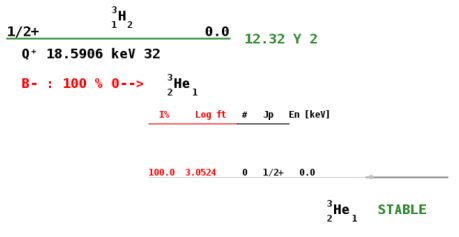
\includegraphics[width=0.47\textwidth]{2Introduction/esquema_niveles_energeticos.png}}
  \subfloat[Graphic representation of tritium decay \cite{TritiumDecayImage}]{
   \label{fig:GraphicDesintegration}
    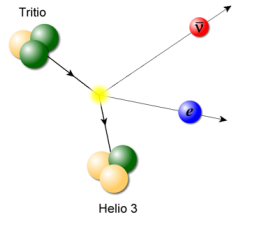
\includegraphics[width=0.53\textwidth]{2Introduction/representacion_desintegracion.png}}
 \caption{Tritium decay}
 \label{fig:TritiumDecay}
\end{figure}

The energy that is released in this nuclear reaccion is constant, $18.6~\keV$, but it is divided between the products of this reaccion. Therefore not all beta particle (electrons) will have the maximum energy. This is what we can see in the figure \ref{fig:TritiumDecaySpectrum}, which is the energetic spectrum of the electrons which are emitted in the tritium decay. The maximum energy of this electrons is $18.6~\keV$ (when beta particles have all the energy), which is the endpoint energy of this spectrum, the average energy is $5.7~\keV$ and the most likely value is slightly below of the average energy, around $4.5~\keV$.

\begin{figure}[hbtp]
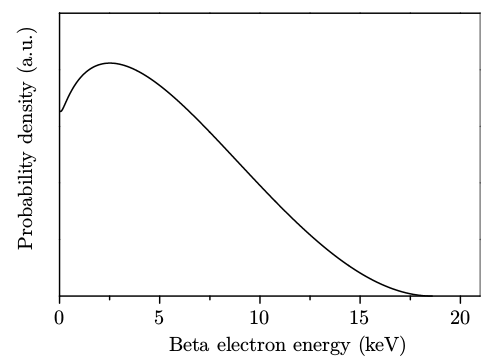
\includegraphics[scale=0.6]{2Introduction/Espectro.png}
\centering
\caption{Energy spectrum of tritium electrons ~\cite{TesisTritio}\label{fig:TritiumDecaySpectrum}}
\end{figure}

Keep in mind that, although the helium isotope is stable, it will be exited immediately after this decay. As a consequence, after the tritium $\beta^-$ decay, we will have a subsequent dexcitation of the $\ce{^{3}He}$ which will produce fotons, $\gamma$, with several well-defined energies that correspond to their energy levels, X-rays. COMPROBAR... It doesn't affect directly to our detector due to the efficiency of our detector at those wavelenghts, as we will se in the chapter \ref{}, section \ref{},  but it could be affect indirectly. BUSCAR ESTAS ENERGÍAS Y VER SI SON TAN DIFERENTES COMO PARA NO AFECTAR DIRECTAMENTE O SE PARENCE A LAS DEL TRITIO Y SI AFECTAN DIRECTAMENTE.

The releasing energy, which is produced in the tritium decay, is very little. In fact, it is the radioactive isotope with the lowest energy released in its $\beta$ disintegration \cite{TritiumHandling}. As a consequence the $\beta$ particles which is emitted in this tritium decay will have a very little mean free path as you can see in the table \ref{MeanFreePathTritium}.

\begin{table}[htbp]
\begin{center}
\begin{tabular}{|c|c|c|}
\hline
Material & Energy ($\beta$)(keV) & Penetration Depth \\
\hline \hline \hline
$\ce{\ce{^{3}_{1}H_2}}$, STP & 5.7 & 0.26 cm \\ \hline
$\ce{\ce{^{3}_{1}H_2}}$, STP & 18.6 & 3.2 cm \\ \hline
Air, STP & 5.7 & 0.036 cm \\ \hline
Air, STP & 18.6 & 0.45 cm \\ \hline
\parbox{10em}{\centering Water, soft tissue\\  (solid matter whose \\  density is $1~\gram\cdot\cm^{-3}$)} & 5.7 & 0.42 $\mu\meter$\\ \hline
\parbox{10em}{\centering Water, soft tissue\\  (solid matter whose \\  density is $1~\gram\cdot\cm^{-3}$)} & 18.6 & 5.2 $\mu\meter$ \\ \hline
\end{tabular}
\caption{Mean Free Path of tritium isotope for several energies~\cite{TritiumHandling}}
\label{MeanFreePathTritium}
\end{center}
\end{table}

On the one hand, it means that the tritium electrons is easily stopped even for simply walls like our clothes, the laboratories gloves or even the our skin it-self, that's, the radioactive hazard is low. Nevertheless, the danger of tritium is increased when tritium is ingested or inhaled because if it has enough radiactivity it can affect to our internal organs because it has a high biologic life time, $9.5$ days \cite{TritiumHandling}, time during which tritium remains in our body and we will be receiving dose due to tritium radiation. Therefore, their health hazard is high.

On the other hand, this short mean free path will be a problem when we try to detect tritium and due to that, there are some limitations which we will have to take into account when we design our detector. 

Tritium has different physical properties than other natural isotopes of the hydrogen like different boilling points as you can see in the table \ref{BoillingPoints} or the property of auto-radiolysis which only happens when radioactive elements are presented. The auto-radiolysis exists because the energy released in tritium decay is larger than the energy bond of oxigen and hydrogen in water molecules ($5.2~\eV$) or the ionization energy of water molecules ($12.6~\eV$) so it can break up these molecules \cite{AutoRadyolisis}. Due to the auto-radiolysis, some radicals appear in the water whose corrosivity is increased.

\begin{table}[htbp]
\begin{center}
\begin{tabular}{|l|l|l|}
\hline
Molecule & Boiling point (for gases) ($\kelvin$) & oxidation form\\
\hline \hline \hline
$\ce{H_2}$ & 20.39 & $\ce{H_2 O}$ \\ \hline
$\ce{HD}$ & 22.14 & $\ce{HDO}$ \\ \hline
$\ce{HT}$ & 22.92 & $\ce{HTO}$ \\ \hline
$\ce{D_2}$ & 23.66 & $\ce{D_2 O}$ \\ \hline
$\ce{DT}$ & 24.38 & $\ce{DTO}$ \\ \hline
$\ce{T_2}$ & 25.04 & $\ce{T_2 O}$ \\ \hline
\end{tabular}
\caption{Gas molecules of hydrogen isotopes and their boiling points}
\label{BoillingPoints}
\end{center}
\end{table}

Although tritium has different physical properties it has almost the same chemical behaviour than other hydrogen isotopes. Tritium, like hydrogen, is a gas at standard conditions of temperature ($273~\kelvin$) and preassure ($1$ atm) forming a two-atom molecules which can be $\ce{HT}$, $\ce{DT}$ and $\ce{T_2}$. It can become in tritium water through oxidation and exchange reactions as you can see in the following chemical ecuations\cite{TritiumHandling}:

\begin{equation}
\begin{split}
& Oxidation: \qquad \qquad \qquad \qquad \qquad \qquad Excahnge\\
& 2\cdot{}\ce{HT} + \ce{O_2} \rightarrow 2 \cdot{} \ce{HTO} ~ \quad \qquad \qquad \qquad \ce{HT} + \ce{H_2 O} \rightarrow \ce{H_2} + \ce{HTO}\\
& 2\cdot{}\ce{T_2} + \ce{O_2} \rightarrow 2 \cdot{} \ce{T_2 O} \qquad \qquad \qquad \qquad \ce{T_2} + \ce{H_2 O} \rightarrow \ce{HT} + \ce{HTO}
\label{OxidationExchange}
\end{split}
\end{equation}

Due to this chemical similarity tritium water can performe the same chemical process than non-radiactive water, some times with higher rate if the tritium concentration is high enough to catalyze the reaction. Its biological hazard comes from this chemical similarity since tritium water is able to substitute normal water in human body. On top of that, tritium water has a higher absorption in human body, around 99\%, than tritium gas, whose absorption in the human body is less than $5 \cdot 10^{-3}\%$  by inalation or practically negligible by skin absorption \cite{TritiumHandling} so it is more dangerous.\label{sec:TritiumProperties}
	\newpage
	
	\section{State-of-the-art in tritium detection}
	Measurement of tritium activity is one of the systematic environmental controls that have been carried out for dozens of years around nuclear power plants during their energy production and around nuclear research facilities.

As a consequence, this measurement has been attempted with many different technologies so far in order to improve the state of the art of each time. The most researched techniques are summarized in the table \ref{DifferentThecnics}.

\begin{table}[htbp]
\begin{center}
\begin{tabular}{|c|c|c|c|c|}
\hline
 & LSC & IC & Calorimetry & BIXS\\
\hline \hline \hline
\parbox{5em}{\centering Measured\\ quantity} & \parbox{5em}{\centering Scintillation\\ photons} &  \parbox{5em}{\centering Ionization\\ current} & heat & X-rays\\ \hline
LDL & $\sim\becquerel$ & $10-100~\kilo\becquerel$ & $\sim~\giga\becquerel$ & $\sim~\mega\becquerel$ \\ \hline
Sample form & Liquid & Gas, vapor & All & All \\ \hline
%Disadvantages & & Gas, vapor & All & All \\ \hline
\end{tabular}
\caption{State-of-the-art in the tritium detection for different technics~\cite{TesisTritio}}
\label{DifferentThecnics}
\end{center}
\end{table}

Nowadays, the most used technic for mesuring tritium in water is the LSC. It consists of mixing a liquid sample (some ml for environmental measurements or less for higher activities) with liquid scintillator. In our laboratories, LARAM, at the University of Valencia, this mixture is made in a ratio of 50:50 \cite{LSCLARAM} but it will depend on each system and each sample \cite{LSCothers} \cite{HofstetterSeveral}. In this technic, the $\beta$ energy that is emitted from the sample excites the molecular energy levels of the liquid scintillator and it is quickly desexcited emitting several photons with a well-know energy (fluorescence), normally in the visible range. Finally these photons are detected with photosensors, processed and analysed.

This technic has a very good detection capability and precision (LDL for tritium better than $1~\becquerel/\liter$ \cite{0.6Bq_L}) but it has some problems. On the one hand it need too time for taking a mesurment (more than $2$ days) and, on the other hand, although this sample could be non-radiactive, it contain tolueno which is a toxical chemical waste so we need to follow a special protocol for removing this samplex. On top of that all these technics need special staff for sampling, chain-of-custody and lab analysis which consum economical and time resources. In order to avoid the last problem a monitor of tritium with LSC has been studied \cite{OnlineLSC} but the other problems still remain. 

The ionization chamber (IC) is based on a gas chamber (sample) which contains electrodes connected to different voltage. This electrodes recover the ionization current that is produced due to the $\beta$ radiation. It is a simple and fast system, but the problem is that on the one hand it has too high LDL, more than $ 10~\kilo\becquerel$, and, on the other hand, it needs the state of the sample to be gas or steam \cite{IonizationChamber1} \cite{IonizationChamber2}.

The calorimetry is based on the measurement of the heat generated due to the tritium radiation \cite{Calorimeter1} \cite{Calorimeter2}. The problem with this technic is that it has a too high LDL, of the order of $\giga\becquerel$, and it needs too long time, more than 2 days, for taking a measurement.

The Beta Induced X-ray Spectrometry (BIXS) is based on the measurement of the bremsstrahlung with PMTs of \ce{NaI} \cite{XRays1} \cite{XRays2} or with Silicon Drift Detector (SDD) \cite{Bremstrahlung} produced due to the tritium radiation. The problem with this technic is that it has too high LDL, of the order of $\mega\becquerel$.

There are many more different methods for tritium detection, although they are less used or less experimentally developed, each one with their own problems for our objective. For example,  APD \cite{APD}, which we cannot use in our case because they cannot function in contact with water, the mass spectrometry \cite{Spectrometry}, which needs to store the sample several months before taking the measurement or Cavity ring spectroscopy \cite{Ring}, which requires a special optical configuration that is not possible outside the laboratory.

We have to keep in mind that all these techniques are offline methods that take too long to finish the process of taking measurements which include sample taking, sending the sample to the lab, analyzing of the sample so we cannot use them for tritium monitoring. LSC is the only technic which has a LDL enough low to verify the compliance with the established limit, $100~\becquerel/\liter$. Therefore we will explore this area but, in order to avoid the problems related with this technic (off-line results, no-reusable liquid scintillator and the chemical toxic wastes) we will delve in solid scintillators. There are several studies that have been done so far which intend to do the same as we want with this project, to create a quasi-real time monitor of low tritium activities in water based on solid scintillation:

\begin{itemize}

\item{} First study was done by M. Muramatsu, A. Koyano and N. Tokunaga in 1967 who used a scintillator plate read out by two PMTs in coincidence \cite{Muramatsu}.

\item{} The second study was carried out by the A. A. Moghissi, H. L. Kelley, C. R. Phillips and J. E. Regnier in 1969 that used one hundred plastic fibers coated with anthracene powder and read out by two PMTs in coincidence \cite{Moghissi}.

\item{} Third study was performed by R. V. Osborne in 1969 who used sixty scintillator plates stacked read out by two PMTs in coincidences \cite{Osborne}.

\item{} Fourth study was done by the A. N. Singh, M. Ratnakaran and K. G. Vohra in 1985, who used a scintillator sponge read out by electronic coincidence \cite{Ratnakaran}\cite{Ratnakaran2000}.

\item{} Fifth study was carried out by K. J. Hofstetter and H. T. Wilson in 1991, who did different experiments for testing different shapes of scintillator plastic like several sizes of beads, fibers, etc. The better result which Hofstetter got for solid plastic scintillator was a efficiency of the order of $10^{-3}$ \cite{Hofstetter1}\cite{Hofstetter2}.

\end{itemize}

\begin{table}[htbp]
\begin{center}
\begin{tabular}{|c|c|c|c|c|}
\hline
 & \parbox{6em}{\centering Efficiency, $\eta_{det}$\\ $(cps/(\kilo\becquerel/\liter))$}  & \parbox{5em}{\centering Surface\\ $F_{sci}$ ($\cm^2$)}  & \parbox{5em}{\centering Specific efficiency\\ $\varepsilon_{det}=\eta_{det}/F_{sci}$} & LDL ($\kilo\becquerel/\liter$)\\
\hline \hline \hline
Muramatsu & $3.85 \cdot 10^{-4}$ & $123$ & $3.13 \cdot 10^{-6}$ & $370$ \\ \hline
Moghissi & $4.5 \cdot 10^{-3}$ & $>424.1$ & $<1.06 \cdot 10^{-5}$ & $37$ \\ \hline
Osborne & $0.012$ & $3000$ & $4 \cdot 10^{-6}$ & $37$ \\ \hline
Singh & $0.041$ & $3000$ & $1.37 \cdot 10^{-5}$ & $<37$ \\ \hline
Hofstetter & $2.22 \cdot 10^{-3}$ & $\sim~100$ & $<2.22 \cdot 10^{-5}$ & $25$ \\ \hline
\end{tabular}
\caption{Results of different scintillator detector for tritium detection~\cite{TesisTritio}}
\label{PlasticScinTritium}
\end{center}
\end{table}

%COMPROBAR QUE ESTAN BIEN TODOS LOS DATOS (sobretodo areas, lo otro esta comprobado. A lo mejor puedo calcular el area del ultimo caso)

The results of these experiments are sumarized in the table \ref{PlasticScinTritium}. We can see in the first column that the intrinsic detector efficiency, $\eta_{det}$, is very different in these experiences. As we know that, in this type of detectors, one of the most important factor, which affect to the efficiency, is the active surface of the plastic scintillator, $F_{sci}$, and we can see in the second column that it is very different en each detector, we use the specific detector efficiency (third column), in order to compare these experiments, that's, the efficiency normalized to this active surface. Now we can check that, effectively, these specific efficiencies are quite similar. On top of that we can check that the better specific efficiency was obtained for Moghissi who used scintillating fibers. This is a good point which justify our choice about using of fibers like a scintillator. Finally we can see in the last column that the LDL in all these experience are more or less similar and, they are too high for our aim. 

To sum up with solid scintillator detectors we can practically avoid all the different problems which other techniques have. The only problem which still remain is that they have a too high LDL. Developing a detector which overcome these LDL is an essential study right now in order to monitoring the tritium levels.\label{sec:StateOfTheArt}
	\newpage
	
	\section{Tritium project and Tritium detector}
	As we have seen in the section \ref{sec:StateOfTheArt}, the current technics which exist nowadays have either higher LDL than the limit established by Council Directive, $100~\becquerel/\liter$, or they are a off-line method (too slow) so those methods cannot be used for tritium monitoring in quasi-real time. 

As a result of these limitations appear the \textit{Tritium} project \cite{TRITIUM}, whose title is "Design, construction and commissioning of automatic stations for quasi-real time monitoring of low radioactive levels of tritium in water".

This project has been funded by Interreg Sudoe program of the EEC in the 2016 call with the reference number SOE1/P4/EO214. The purpose of this project is the development of a tritium monitor in quasi-real time. This monitor consists of a ultra pure water system, which prepare the sample before we introduce it in our detector, the tritium detector where the tritium measure will be done, the active veto and the pasive shielding which reduce the natural background of our tritium detector and several types of electronic which control all these parts of the monitor, analyze the tritium measurement and will send an alarm if the limit of $100~\becquerel/\liter$ is overcome.

The tritium detector is based on measurements of low energy beta radiation from the radioactive decay of tritium. For doing this task this detector consists of scintillator fibers, that we put directly in contact with water which can contain tritium. We need to put both, scintillator fibers and tritium water, in contact due to such a low mean free path of tritium electrons (table \ref{MeanFreePathTritium} of the seccion \ref{sec:TritiumProperties}). Then, the photons produced on this fibers will be read out by several photosensors. The photosensors which we have tested in this experiment are photoelectron multiplier tubes (PMT) and silicon photoelectron multiplier (SiPM) arrays. 

The difficulty when we try to measure tritium is to distinguish these signals from the background. This is because tritium signals are small since tritium events has low energy ($\sim~\keV$) and this is the energy range in the spectrum where there are more background counts (the lower energy, the more background events). We will use coincidence techniques in order to reduce the counts from the background.

It is important to check the water tightness of each prototype because if the water reaches the photosensor it will be irreparably damaged. On top of that if we use high concentrations of tritium in water for laboratory tests we can contaminate this laboratory, which could be dangerous for the healthy of the workers and it could spoil measurements of future experiments.

Finally this monitor will be installed in the Arrocampo dam, Almaraz, Spain, where the Almaraz nuclear power plant release the water which is used in their cooling system, Figure \ref{fig:Arrocampo}. This NPP has two nuclear reactors whose type is PWR. This dam is located near the Tajus river, which is the largest river in Spain, $1007~\kilo\meter$. This river cross from Aragon (Spain) to Lisbon (Portugal) and flows into the atlantic ocean. This river is used for an important quantity of animals, plants and even humans because the water of this river is used as drinking water by the spanish and portuguese people. Therefore the international cooperation in order to maintain the quality of this water is very important.

\begin{figure}[hbtp]
 \centering
  \subfloat[Arrocampo dam and Almaraz Nuclear Power Plant]{
   \label{fig:Arrocampo_Dam}
    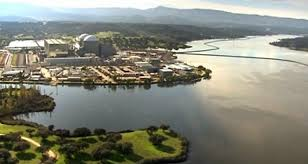
\includegraphics[width=0.47\textwidth]{2Introduction/ArrocampoDam.jpeg}}
  \subfloat[Tajus river along Spain and Portugal]{
   \label{fig:TajusRiver}
    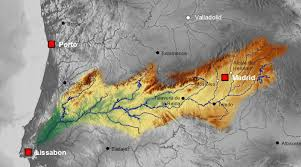
\includegraphics[width=0.53\textwidth]{2Introduction/RioTajo.jpeg}}
 \caption{Arrocampo dam, Almaraz NPP and Tajus river}
 \label{fig:Arrocampo}
\end{figure}

The \textit{Tritium} collaboration is a international group consisting of a consortium of 6 different southwestern european institution of 3 different countries: The University of Aveiro, in Portugal, The University of Bordeaux and the CNRS  (Section Aquitaine-Limousin), in France and the University of Extremadura, \textit{Junta de Extremadura} and University of Valencia, in Spain.

FOTOO TRITIUM

Each institution has focused in the development of a different part of all this project:
\begin{itemize}
\item{} First, the Extremadura group has developed and installed the ultra pure water system with wich we get water with very low conductivity, $\sigma \approx 10 ~\mu S / \cm$. The conductivity of the water before the cleaning proces is around $ 1000 ~\mu S / \cm$. This clean process is very important for two reasons. On the one hand, it is important for maintaining our detector very clean, which is a critical point. On the other hand, it's important because with this process we reduce the natural background since we remove several natural radiactive isotopes that there are in this water (except tritium) such as $\ce{^{222}Rn}$, $\ce{^{40}K}$ or $\ce{^{137}Cs}$. This system will be explained in the chapter \ref{chap:Ultrapure}.

\item{} Second, french group has develop the pasive shielding where our detector will work inside. It is based in ultra radiopure lead with very low intrinsic activity. The objective of this pasive shielding is to reduce the external natural background that affect to our system, for this reason we use lead. Obviously, this shielding doesn't have to affect to the measurement of our system, for this reason we use radiopure elements with very low intrinsic activity. This shielding will be explained in the chapter \ref{chap:Shields}, section \ref{sec:PasiveShields}.

\item{} Third, The Portugal and Spanish people has developed the simulations about this system. The program which we have used in this project is GEANT 4, which is a simulation package. It consiste in a extensive C++ library with which we can design the geometry of our detector, the physical processes which happen there, etc. This simulation will be explained in the chapter \ref{chap:Simulations}.

\item{} Lastly, The Portugal and Spain people has collaborated for designing, developing and building four different prototypes of tritium detector and active vetos for removing cosmic events. These prototypes and vetos will be explained in the chapter \ref{chap:Prototypes}.

\end{itemize}

The tritium level which we want to mesure follow the ALARA principle (As Low As Possible Achievable) and to get it there are important characteristics which our tritium detector must have:

\begin{itemize}

\item{} \textit{Compact}. This is important because in the place where this detector will be installed the useful space that we can use is finite.

\item{} \textit{Thin active volume and large active area}. On the one hand, we have to take into account that, as we have seen in the table \ref{MeanFreePathTritium} of the seccion \ref{sec:TritiumProperties}, the mean free path of the $\beta$ particle of tritium decay is very low so we need to work with thin active volumes. In the practice, Active thickness beyond the mean free path of the tritium will only contribute to the background. On the other hand, as we have checked in the seccion \ref{sec:StateOfTheArt} the efficiency of this type of detector scales with the active area so we need to design our detector with the largest possible active area.

\item{} \textit{High sensitivity to tritium}. We are going to work with low tritium activities so we need to reduce as much as possible the non-detected tritium events.

\item{} \textit{High specificity to tritium}. We need that our detector is able to distinguish the tritium signal of the signal of other radiactive elements which can be present in the initial sample.

\item{} \textit{Quasi-real time response}. As we have seen it is important that our sistem can work in quasi-real time in order to detect any problem as fast as possible. 

\item{} \textit{Rugged system}. Finally, we have to take into account that our objective will be installing an automatical system which will work during a lot of years without specialized people so we need that our monitor are rugged. 

\end{itemize}

In order to get the measurement in quasi-real time we need to work \textit{in situ}, that's, we need that our detector is able to work in the same place that we take the sample. Whit the work \textit{in site} we achieve:

\begin{itemize}
\item{} a faster monitor because we eliminates the process of taking the sample, the chain-of-custody until this sample arrive to this laboratory and the complexity which involve these tasks. 

\item{} a better monitor since if we can work \textit{in site}, our measurements can be more frequent hence we will can identify cahnges in the activity earlier.

\item{} a cheaper monitor because we have not only the material costs attached to the sample collection, chain-of-custody of this sample, shipping of this sample to the laboratory, etc. but we have also eliminated the costs attached to the specialized staff who are involving in these tasks. Our detector will only need frequent calibrations each time in order to ensure its correct operation.

\item{} a safer monitor since the personal exposure dose is reduced and the changes in activity are detected fastly. On top of that we remove the possibles mistakes which can be done by specialized staff.

\end{itemize} \label{sec:TritiumProject}
	\newpage
	
	\section{Work scheme}
	%This thesis is build up as follow:...



The objetive of this three-phase project was design, develop and instalation and commisioning a automatical system capable of detection tritium which we find in the water that is used by the nuclear power plants for their cooling system. The initial idea was quantifying its activity in quasi-real time before discharging it into public rivers or seas. 

We are speaking all the time about getting the measurement in quasi-real time, that is, in less of 10 minuts but what about the real time? It is obviously imposible because we are mesuring the activity, I mean, we are counting tritium decays in samples with low activities (supposedly less than $100~\becquerel/\liter$) so we need some time in order to get enough stadistic with which we can distinguish the tritium signal to the background in our system.

In order to get the measurement in quasi-real time we need to work \textit{in situ}, that's, we need that our detector is able to work in the same place that we take the sample. The reason of this fact is because if we need to move the sample we lose a lot of time (1 or 2 days in some cases). Furthermore if we avoid to move the samples we get a:

\begin{itemize}
\item{} faster detector because we eliminates the process of taking the sample, the chain-of-custody until this sample arrive to this laboratory and the complexity which involve these tasks. 

\item{} better detector since if we can work \textit{in site}, our measurements can be more frequent hence we will can identify cahnges in the activity earlier.

\item{} cheaper detector because we have removed all the cost associated with the sample collection, chain-of-custody of this sample, shipping of this sample to the laboratory and analysis thereof there. Not only we have eliminated the material costs attached to this tasks (material, transport, etc) but we have also eliminated the costs attached to the specialized staff who are involving in these tasks. With our detector we will only need frequent calibrations each time, which we consider suitable, in order to ensure the correct operation of this detector

\item{} safer detector since the personal exposure dose is reduced and the changes in activity are detected fastly. On top of that we remove the possibles mistakes which can be done by specialized staff who follow each protocol of this tasks.

\end{itemize} 

Dividiremos este trabajo en seis partes:
\begin{enumerate}
\item{} En primer lugar, se realizará un estudio sobre las fibras centelleadoras para  determinar  el protocolo de manipulación para obtener un  procedimiento de preparación de  un haz de fibras centelleadoras con un buen rendimiento óptico. 

\item{} En segundo, lugar estudiaremos el procedimiento de calibración de los SiPM,  fundamental para el experimento.  No se necesita realizar una calibración de los PMT, paso igualmente importante al anterior, ya que este trabajo fue realizado recientemente por otro componente del grupo.

\item{} En tercer lugar, se describirá  el primer prototipo diseñado, formado por un haz de 35 fibras centelleadoras sin clad leídas por PMT,  incluyendo el protocolo del proceso de llenado con agua tritiada que tuvo que ser desarrollado para cumplir los requisitos de protección radiológica y evitar contaminación accidental,  y los  resultados obtenidos con el mismo.

\item{} En cuarto lugar, se presentarán las simulaciones realizadas con el programa de Geant4 en una configuración sencilla.

\item{} En quinto lugar, se expondrán aspectos a estudiar en el futuro inmediato y en etapas posteriores, durante la Tesis Doctoral. 


\item{} Se presentarán, finalmente, los resultados, logros y conclusiones alcanzadas en el desarrollo del  trabajo.

\end{enumerate}\label{sec:WorkScheme}
	\newpage

%\newpage
%\chapter{Scintillator fibers} \label{chap:GeneralFibers}
%\input{./Sections/4Fibras}
	%\section{Introduction}\label{sec:IntroductionFibers}
	%%Para llevar a cabo esta caracterización de los SiPM se ha necesitado de la instrumentación que se especifica a continuación:

\begin{enumerate}
\item {} En primer lugar se necesitaba una \textbf{cámara de control de temperatura}. 
\newline
Dado que la cámara existente en el laboratorio del IFIC no estaba configurada, tuvo que utilizarse la cámara que se encontraba en el IFIMED. Esta cámara (marca DYCOMETAL, modelo CCM 81) se presenta en la figura~\ref{sistematemperatura} izquierda.
Este sistema dispone de un panel de control con el que se puede especificar la temperatura y humedad a la que queremos trabajar en el interior de la cámara. Sin embargo, para asegurar el correcto funcionamiento de la cámara, debíamos trabajar siempre en la zona 1 de acuerdo al diagrama de estados  en la ficha técnica de la cámara, mostrado en la figura~\ref{sistematemperatura} derecha. Posee un interior metálico que permite una rápida estabilización ante posibles cambios de las condiciones en su interior y, además, actúa a modo de jaula de Faraday. 

\begin{figure}[htb]
\centering
{
%\subfloat[Espectro de emisión]
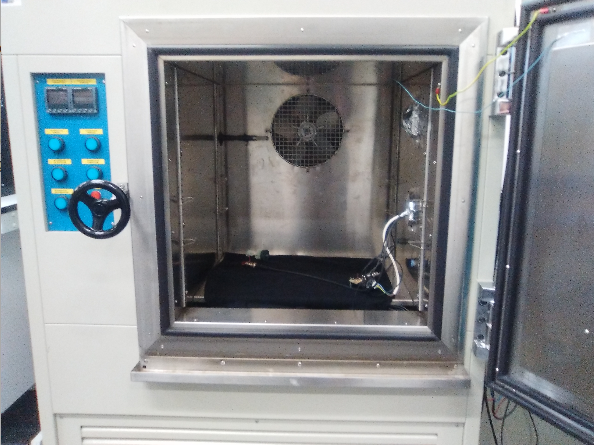
\includegraphics[scale=0.3]{InteriorTemperatura.png} 
}
{
%\subfloat[Espectro de emisión]
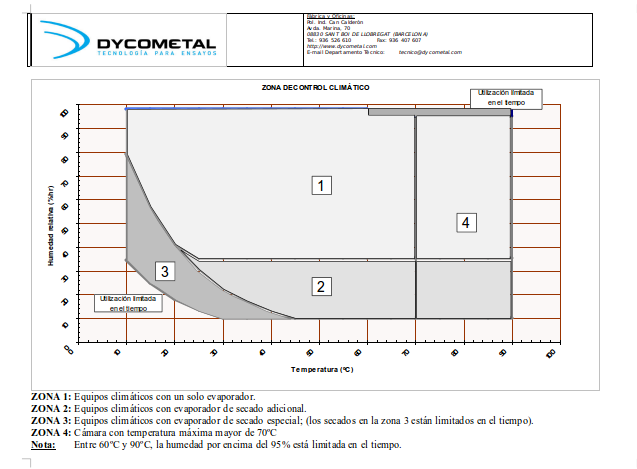
\includegraphics[scale=0.3]{FichaTecnica.png} 
}
\caption{Sistema de control de temperatura y diagrama de estados~\cite{dycometal}\label{sistematemperatura}}
\end{figure}

La incertidumbre  del punto de trabajo es $0.1~\celsius$ para la temperatura y $0.5\%$ para la humedad relativa. Estas incertidumbres se determinaron observando la oscilación  máxima en la pantalla del panel de ambos parámetros tras llegar a la estabilidad en el interior de la cámara.
En el interior de esta cámara se encontraba nuestra fuente de luz que proporcionaba la señal de entrada del sistema que pretendíamos medir con el SiPM, el propio SiPM, la tarjeta de conversión intensidad-voltaje y cableado que hacía posible la interacción con estos dispositivos. Además, hay que tener en cuenta que esta cámara no actuaba como caja negra, por lo que para conseguir reducir la posible entrada de luz del exterior se taparon todas las posibles entradas de luz del sistema con cinta metálica y, además, se cubrió el dispositivo con una tela negra especial. Con todo esto, conseguimos reducir el fondo del sistema hasta un nivel adecuado.

\item {} En segundo lugar necesitamos instrumentos nos permitiesen alimentar tanto el SiPM como la tarjeta de conversión intensidad-voltaje. Se utilizo  un \textbf{electrómetro} (marca KEITHLEY, modelo 6517B) para alimentar el SiPM y un \textbf{generador de tensión} (marca ISO-TECH, modelo IPS-4303) para alimentar la tarjeta de conversión.

Se utilizo el electrómetro para el SiPM, ya que este dispone de una fuente de tensión de hasta $1000\volt$. Por el contrario, el ISO-TECH sólo dispone de una tensión máxima de $30~\volt$. Poseen una resolución  inferior al milivoltio e inferior a $0.1~\volt$ respectivamente, suficiente para que las ganancias que dependen del voltaje (ganancia del SiPM y de la tarjeta respectivamente) no varíe cuando fijamos el voltaje.

\item {} En tercer lugar, se necesitaba una \textbf{fuente de luz} que simulase la emisión de los fotones de la fibra centelleadora. 
\newline
Se utilizó un \textbf{diodo LED} (de la empresa Roithner Laser technik) que emite fotones de una longitud de onda de $435~\nano\meter$~\cite{datasheetLED}, en la zona del azul. Esta es la longitud de onda que necesitamos en nuestro experimento para calibrar el SiPM, ya que corresponde a la longitud de onda a la cual el espectro de emisión de las fibras centelleadoras BCF-12 tiene su máximo.

%\newpage
\item {} En cuarto lugar, para alimentar este diodo LED, se necesitó un \textbf{generador de pulsos} (marca Agilent, modelo 33250A). Este generador de señales nos permite especificar la forma del pulso que pretendemos proporcionar y sus características. Este tenía que ser capaz de formar un pulso suficientemente estrecho para que el SiPM detectase unos pocos fotones. 

En concreto alimentamos el diodo LED con un pulso cuadrado. Los parámetros que nos permite especificar el generador de señales para un pulso de esta forma son frecuencia (o período), high level (o amplitud), low level, offset, anchura del pulso y tiempo de atenuación. Para nuestro estudio, los valores de estos parámetros que nos daban un mejor resultado desde el punto de vista experimental fueron una frecuencia de $20~\hertz$, high level de $2.275~\volt$, low level de $1~\volt$, offset de $1.638~V_{dc}$, anchura del pulso de $12~\nano\second$ y tiempo de atenuación de $5~\nano\second$.
Este generador de señal nos proporciona una segunda señal, denominada señal de sincronización, la cual podemos utilizar como trigger para determinar el instante de tiempo en el que se activa la señal luminosa.

\item {} En quinto lugar, utilizamos un \textbf{SiPM} para detectar los fotones emitidos por el LED. En concreto, se utilizó el modelo S13360-1375CS de Hamamatsu Photonics, que es un fotomultiplicador cerámico de silicio que presenta una ganancia típica de $G=4 \cdotp 10^6$ y una eficiencia de fotodetección típica del $50\%$ a $25~\celsius$ y $V_{ov}=V_{op}-V_{bd}=3~\volt$. Su campo espectral  es de $[270-900]\nano\meter$~\cite{datasheet SiPM}.
Este SiPM compuesto por un total de $285$ pixels de $75~\micro\meter$ cada uno dando lugar a una superficie total activa de $1.3\times1.3~\milli\meter^2$ frente a su superficie total que es de $6\times5~\milli\meter^2$. Puede verse reflejado en la figura~10 izquierda~\cite{datasheet SiPM}. 

\item {} Hay que tener en cuenta que el SiPM nos proporciona un pulso de intensidad a la salida y  necesitamos convertir este en un pulso de voltaje para, de esta forma, poder introducirla al osciloscopio para realizar el posterior análisis. Para ello emplearemos en sexto lugar una \textbf{tarjeta conversora} de intensidad en voltaje que puede verse reflejada en la figura~\ref{TarjetaSiPM} derecha, en la cual se encuentra el SiPM utilizado conectado a la misma. 

\begin{figure}[htb]
\centering
{
%\subfloat[Espectro de emisión]
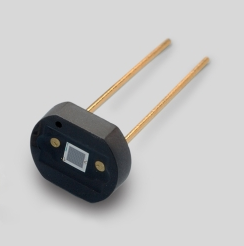
\includegraphics[scale=0.55]{SiPM.png} 
}
{
%\subfloat[Espectro de emisión]
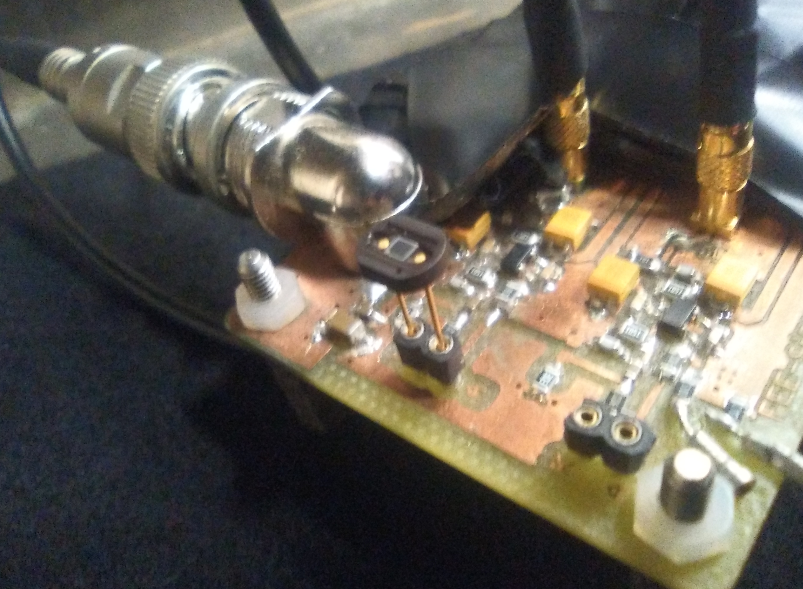
\includegraphics[scale=0.23]{tarjeta.png} 
}
\caption{SiPMs (izquierda) y tarjeta de alimentación conversora intensidad-voltaje (derecha)\label{TarjetaSiPM}}
\end{figure}
Esta es una tarjeta desarrollada en el marco del proyecto NEXT.Esta consiste de dos entradas donde podemos conectar dos SiPM distintos. La tarjeta contiene el circuito  de la figura~\ref{esquemacircuitotarjeta} para cada SiPM:

\begin{figure}[hbtp]
\centering
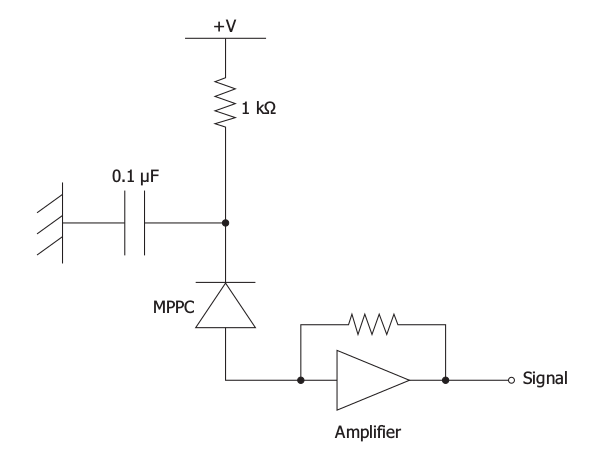
\includegraphics[scale=0.3]{CircuitoTarjeta.png}
\caption{Circuito de una tarjeta tipo~\cite{datasheet SiPM}\label{esquemacircuitotarjeta}}
\end{figure}
\newpage
La tarjeta tiene una ganancia de $G=170$. Este será el valor que utilizaremos en el análisis posterior para calcular la ganancia de los SiPM.

\item {} Seguidamente se observó que, únicamente alimentando la tarjeta, antes de alimentar el SiPM y la led, obteníamos una perturbación externa a nuestro experimento. Esta se presenta en la figura~\ref{Ruido}. 

\begin{figure}[hbtp]
\centering
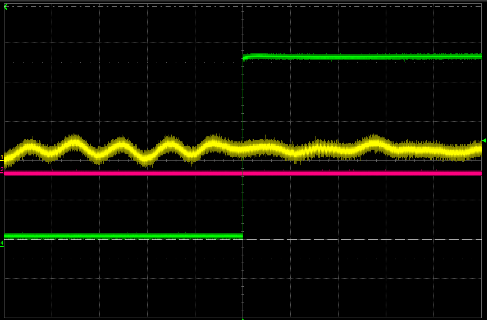
\includegraphics[scale=0.4]{ruido.png}
\caption{Ruido electrónico\label{Ruido}}
\end{figure}
Se intento caracterizar esta señal de perturbación, ajena a nuestro experimento y, a priori, de origen desconocido. Tenía una amplitud máxima de $4~\milli\volt$ y una frecuencia bastante irregular entorno al $\mega\hertz$. Finalmente se vio que era debido por una parte a la emisión producida por la antenas de Radiotelevisión Valenciana y, por otra parte, de las distintos intrumentos electrónicos conectados a la red eléctrica del IFIC, ya que esta posee una toma a tierra bastante irregular. 
Con la presencia de este ruido no podíamos realizar medidas ya que introducía una componente de ruido tal que estropeaba por completo el resultado de la medida. Con el fin de solucionar este problema se dispuso de un \textbf{filtro pasa banda} (GUARD LCD2 650 AP) para eliminar este ruido.

\item {} Finalmente, como se ha mencionado anteriormente, necesitamos una \textbf{manta negra} especial que apantallase la entrada de fotones del exterior, ya que el sistema de control de temperatura no actuaba como caja negra.

Una alternativa podría haber sido introducir una caja negra en el interior del sistema de control de temperatura y introducir el diodo Led, el SiPM y la tarjeta en su interior. Sin embargo de esta forma no conseguimos un control de la temperatura y humedad en su interior.

\end{enumerate}

	
	%\section{Organic and inorganic scintillators}\label{sec:OrganicInorganicFibers}
	%La tarjeta empleada en el sistema (Fig. $\ref{TarjetaSiPM}$) es una tarjeta desarrollada en el marco del proyecto NEXT. La necesidad de ésta, como se ha comentado anteriormente, reside en que la señal de salida de un SiPM es una señal de intensidad y el osciloscopio únicamente puede trabajar con señales de voltaje. Por tanto, para poder analizar esta señal, es necesario utilizar una tarjeta conversora de intensidad en voltaje. Esta consiste de dos entradas donde podemos conectar dos SiPM distintos. La tarjeta contiene el circuito  de la figura~\ref{esquemacircuitotarjeta} para cada SiPM:

\begin{figure}[hbtp]
\centering
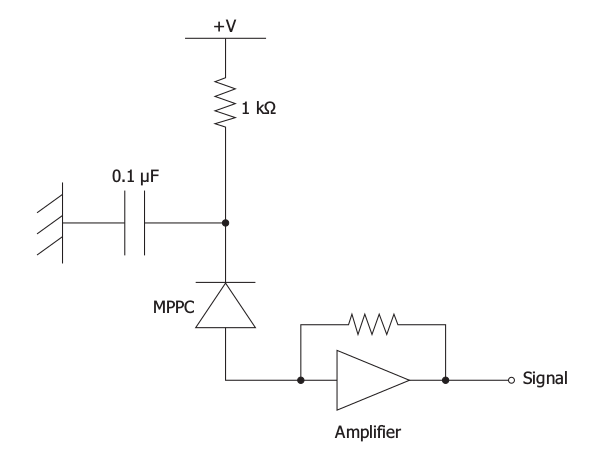
\includegraphics[scale=0.4]{CircuitoTarjeta.png}
\caption{Circuito de una tarjeta tipo~\cite{datasheet SiPM}\label{esquemacircuitotarjeta}}
\end{figure}
La tarjeta tiene una ganancia de $G=110$. Este será el valor que utilizaremos en el análisis posterior para calcular la ganancia de los SiPM.

%Dado que no conocemos su incertidumbre consideraremos este valor como un valor sin error. Esto nos conducirá a obtener una subestimación de la incertidumbre de la ganancia de los SiPM. Sin embargo esto no tiene mayor importancia ya que será un factor constante que afectará por igual a todas las medidas y no estamos buscando determinar la ganancia de los SiPM sino únicamente sus dependencias con el voltaje y la temperatura. 	

	%\section{Scintillator fibers}\label{sec:ScintillatorFibers}
	%La tarjeta empleada en el sistema (Fig. $\ref{TarjetaSiPM}$) es una tarjeta desarrollada en el marco del proyecto NEXT. La necesidad de ésta, como se ha comentado anteriormente, reside en que la señal de salida de un SiPM es una señal de intensidad y el osciloscopio únicamente puede trabajar con señales de voltaje. Por tanto, para poder analizar esta señal, es necesario utilizar una tarjeta conversora de intensidad en voltaje. Esta consiste de dos entradas donde podemos conectar dos SiPM distintos. La tarjeta contiene el circuito  de la figura~\ref{esquemacircuitotarjeta} para cada SiPM:

\begin{figure}[hbtp]
\centering
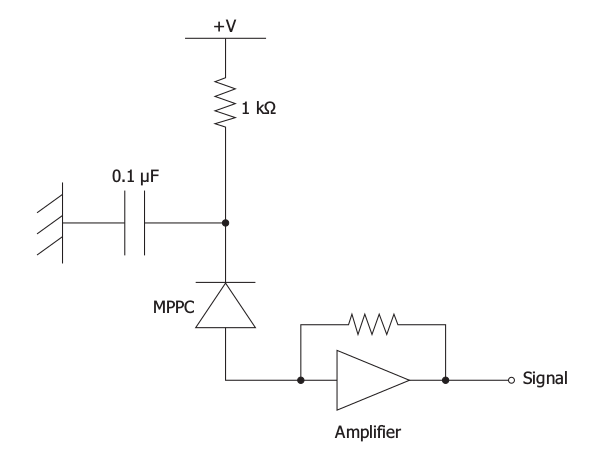
\includegraphics[scale=0.4]{CircuitoTarjeta.png}
\caption{Circuito de una tarjeta tipo~\cite{datasheet SiPM}\label{esquemacircuitotarjeta}}
\end{figure}
La tarjeta tiene una ganancia de $G=110$. Este será el valor que utilizaremos en el análisis posterior para calcular la ganancia de los SiPM.

%Dado que no conocemos su incertidumbre consideraremos este valor como un valor sin error. Esto nos conducirá a obtener una subestimación de la incertidumbre de la ganancia de los SiPM. Sin embargo esto no tiene mayor importancia ya que será un factor constante que afectará por igual a todas las medidas y no estamos buscando determinar la ganancia de los SiPM sino únicamente sus dependencias con el voltaje y la temperatura. 	
	
	%\section{Choice of the comercial scintillator fibers}\label{sec:ChoiceFiber}
	%La tarjeta empleada en el sistema (Fig. $\ref{TarjetaSiPM}$) es una tarjeta desarrollada en el marco del proyecto NEXT. La necesidad de ésta, como se ha comentado anteriormente, reside en que la señal de salida de un SiPM es una señal de intensidad y el osciloscopio únicamente puede trabajar con señales de voltaje. Por tanto, para poder analizar esta señal, es necesario utilizar una tarjeta conversora de intensidad en voltaje. Esta consiste de dos entradas donde podemos conectar dos SiPM distintos. La tarjeta contiene el circuito  de la figura~\ref{esquemacircuitotarjeta} para cada SiPM:

\begin{figure}[hbtp]
\centering
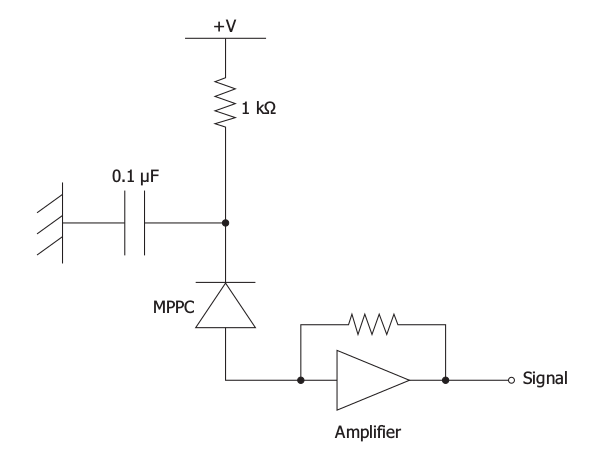
\includegraphics[scale=0.4]{CircuitoTarjeta.png}
\caption{Circuito de una tarjeta tipo~\cite{datasheet SiPM}\label{esquemacircuitotarjeta}}
\end{figure}
La tarjeta tiene una ganancia de $G=110$. Este será el valor que utilizaremos en el análisis posterior para calcular la ganancia de los SiPM.

%Dado que no conocemos su incertidumbre consideraremos este valor como un valor sin error. Esto nos conducirá a obtener una subestimación de la incertidumbre de la ganancia de los SiPM. Sin embargo esto no tiene mayor importancia ya que será un factor constante que afectará por igual a todas las medidas y no estamos buscando determinar la ganancia de los SiPM sino únicamente sus dependencias con el voltaje y la temperatura. 
	
	%\section{Cutting device for scintillator fiber}\label{sec:CuttingFibers}
	%% En resumen, en nuestra prueba de calibración de los SiPM tenemos una caja que actuará como jaula de Faraday, con temperatura y humedad controlada y apantallada en lo posible de la luz del exterior. 

En su interior colocamos un diodo LED que emite fotones de $\lambda=435~\nm$, un SiPM, que emite un impulso de intensidad cada vez que detecte uno o más  fotones  y una tarjeta que convierte este impulso de intensidad en un impulso de voltaje. Finalmente llevamos este impulso de voltaje a un osciloscopio (marca TELEDYNE LECROY, modelo WwaveRunner 625Zi) que lo analiza. 
Una vez en el osciloscopio, la señal que recibimos cuando se enciende el diodo LED es similar a la de la señal superior de la figura~\ref{analisis} (amarilla)~\cite{inftec}. Para el análisis,  se  activa el modo persistencia del osciloscopio con el objetivo de comparar señales de distintas alturas. Estas señales corresponden a distinto número de pixels activados en cada instante de tiempo ya que, como hemos dicho anteriormente, la señal de salida del sistema es la suma de las señales de los pixeles activados. La señal se muestra superpuesta a la señal de sincronización del generador de señales (verde) que nos muestra cuando se ha encendido el diodo LED y que, por tanto, actúa como trigger.

El objetivo ahora es calcular la ganancia del sistema. Dado que únicamente existen dos ganancias en el sistema (SiPM y tarjeta) y conocemos la ganancia de la tarjeta, mencionada en la sección anterior, determinando la ganancia total podremos determinar de forma aproximada la ganancia del SiPM. 

\begin{equation}
G_{tot}=G_{SiPM} \cdotp G_{card} \longrightarrow G_{SiPM} = \frac{G_{tot}}{G_{card}}
\label{ganancias}
\end{equation}

Para medir la ganancia total realizamos una integral del área de cada uno de los impulsos de salida del sistema y guardamos el resultado en un histograma. De esta forma, obtenemos un histograma de las cargas de los pulsos. La ventana temporal sobre la que se integra es aproximadamente una división, que equivale a $500~\ns$. Esta se ajusta con bastante precisión al impulso, algo muy importante para evitar la introducción de fondo (ver figura~\ref{analisis}).

Dado que idealmente el impulso producido por  los pixel son idénticos, el histograma obtenido debería ser  un conjunto deltas de Dirac equiespaciadas. Sin embargo, hay que tener en cuenta que la cascada que produce cada uno de estos fotones detectados en cada pixel esta sometido a fluctuaciones estadísticas. Además, los propios instrumentos de medidas empleados tienen una incertidumbre inherente. Hay que tener en cuenta que también tenemos distintas fuentes de fondo, como la corriente oscura (ruido térmico), fotones de luz del exterior, etc. 
Como resultado de todo esto, lo que obtenemos un conjunto de gaussianas equiespaciadas. En la figura~\ref{analisis} inferior puede verse el resultado de una toma de datos de $25000$ eventos a $25~\celsius$, $60\%$ de humedad y $V_{ov}=3~\volt$,

\begin{figure}[hbtp]
 \centering
 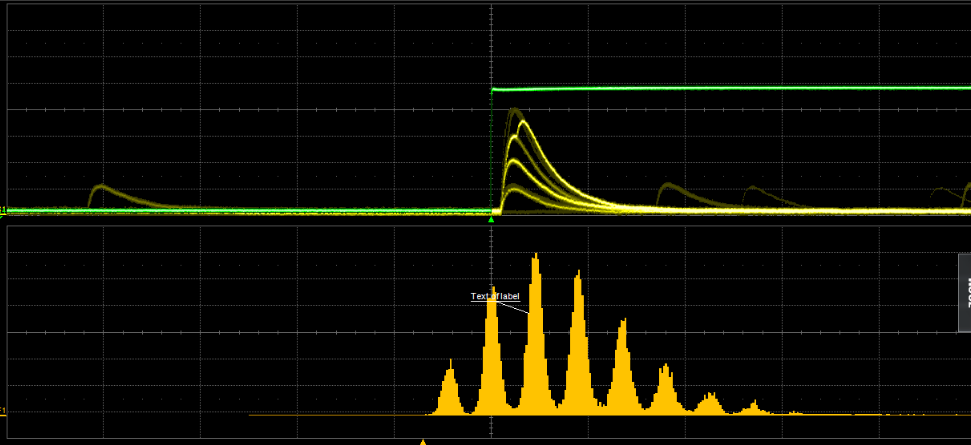
\includegraphics[scale=0.4]{Analisis.png}
 \caption{Captura de las señales en el osciloscopio (arriba) y espectro de carga (abajo)\label{analisis}}
 \end{figure}
donde cada uno de los picos corresponde a la carga de un número de pixels activados (uno, dos, etc.). El primer pico no debe tenerse en cuenta en el análisis, ya que este corresponde al pedestal (cero pixels activados).
 
Hemos desarrollado una macro en ROOT$~\cite{manualROOT}$ que, utilizando la librería TSpectrum (especialmente diseñada para el análisis de histogramas con picos) para obtener la ganancia del sistema. Su diagrama de flujo es el siguiente:
\begin{enumerate}
\item {} Primero la macro lee el fichero de datos, los guarda en una variable de tipo histograma y los representa. La macro termina de leer el fichero cuando no encuentra más valores.

\item {} A continuación, a partir de una función de la librería TSpectrum, busca en este histograma y devuelve el número de gausianas que ha encontrado y su posición.

\item {} Seguidamente ajusta todos los datos del histograma a una recta y solo se queda con las gausianas, cuya norma sobrepasa en altura a esta recta. El objetivo de este paso es que, en casos muy concretos (temperatura alta o luz del laboratorio encendida) tenemos mucho ruido y, aparece un fondo,  que el programa ajusta a una gausiana y, como consecuencia calcula la ganancia de manera incorrecta. Un ejemplo de este caso se muestra en la figura$~\ref{fondogrande}$.

\begin{figure}[hbtp]
\centering
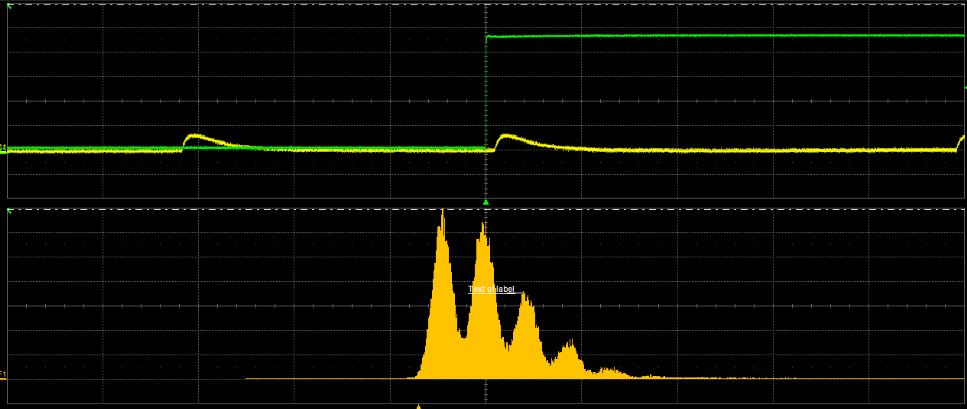
\includegraphics[scale=0.4]{fondogaussiano.png}
\caption{Espectro de carga con mucha corriente oscura\label{fondogrande}}
\end{figure}

\item {} A continuación, ajustamos el espectro a una recta más una suma de $n$ gausianas, donde $n$ es el número de gausianas que superan la recta (calculado en el paso anterior). La necesidad de utilizar una recta es debido a que siempre vamos a tener corriente oscura y otro tipo de fondo que aparecen como una linea base en el histograma, como puede verse en la figura~\ref{analisis}. Podemos apreciar en la figura~\ref{Root} que el ajuste (linea roja) es relativamente bueno. Para determinar si el ajuste es aceptable aplicamos el test $\chi^2$. En este caso se obtuvo un resultado de $\frac{\chi^2}{ndf}=\frac{1276}{223}\approx 5.72$. Vemos que efectivamente, el ajuste lineal representa bien los datos.

\begin{figure}[hbtp]
\centering
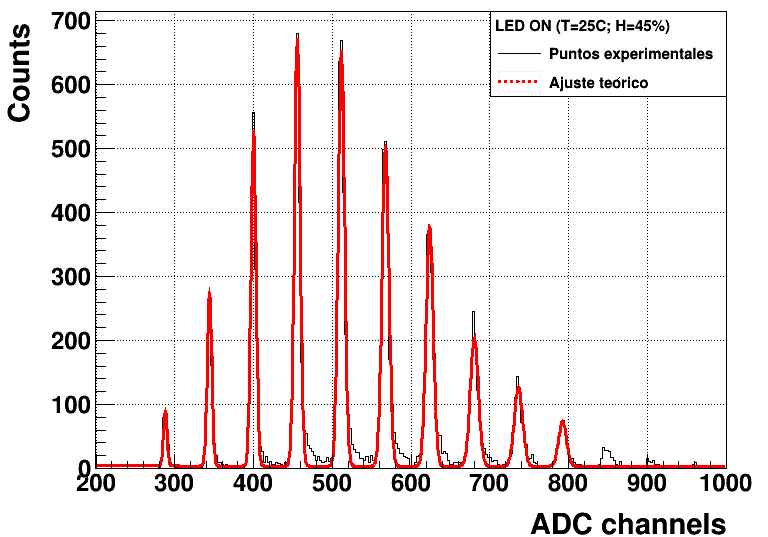
\includegraphics[scale=0.4]{AjusteEspectro1.png}
\caption{ Ajuste de un espectro con la macro de ROOT\label{Root}}
\end{figure}

\item {} Dado que se ha observado que, aun con el tercer paso, existen situaciones límites en que el fondo sigue superando la recta, se ha incluido un paso en la macro en la cual se acepta por teclado uno a uno los picos que serán utilizados en el análisis. Además, la macro calcula la resolución de cada gaussiana y la resolución total, obtenida a partir de la suma cuadrática de la resolución de cada gaussiana. Los valores habitualmente encontrados en los análisis se encuentran en el intervalo $1.5\% - 5\%$, valores bastante aceptables.

\item {} Finalmente, la macro ordena los picos según su posición en el espectro y calcula la ganancia por dos caminos:
	\begin{enumerate}

	\item {} Por un lado se ha calculado la distancia promedio entre sucesivas gausianas del espectro~\cite{Hueso}.
	\begin{equation} 
	Q = G N_\gamma + Q_0 \longrightarrow \Delta Q= Q_{N_\gamma} - Q_{N_\gamma -1}=G N_\gamma+ Q_0 - G(N_		\gamma -1) - Q_0 = G
	\label{gananciametodo1}
	\end{equation}
	Podemos observar que este cálculo corresponde a la ganancia. Hay que tener en cuenta que se han empleado factores de conversión para convertir la posición del pico (inicialmente en unidades de	tensión $\volt$) en unidades de carga $\coulomb$. En concreto, se ha utilizado el factor $\frac{1}{eR}$, donde $R$ es la impedancia de entrada del osciloscopio, $50~\ohm$ y $e$ es la carga del electrón.
	
	\item {} Por otro lado, se ha ajustado a una recta las posiciones horizontales de estas gausianas en el 	espectro frente a el número de píxeles. Esto nos da la siguiente ecuación~\cite{Hueso}:
	\begin{equation}
	Centro\_pico(V) = GeRN_\gamma + k_0
	\label{gananciametodo2}
	\end{equation}
	 Vemos por tanto, que a partir del valor de la pendiente podemos obtener	el valor de la ganancia. La figura~\ref{ajuste} muestra un ejemplo de ajuste de posiciones de gausianas y número de píxeles para el caso de $25~\celsius$, humedad de $45\%$ y $V_{ov}=3~\volt$. Podemos observar que existe	un acuerdo excelente, algo que ocurre prácticamente en la totalidad de los casos. Las barras de error  de este gráfico  no son apreciables en esta  escala.
		
	\begin{figure}[hbtp]
		\centering
		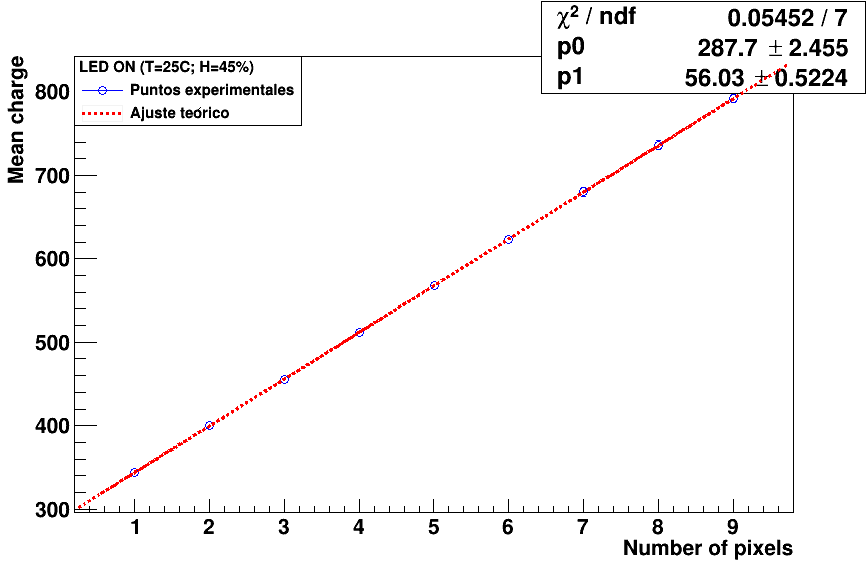
\includegraphics[scale=0.4]{FitPosicionPixels.png}
		\caption{Ajuste carga de las señales del SiPM frente al número de píxeles encendidos\label{ajuste}}
		\end{figure}
			
	\end{enumerate}
	
Para este caso concreto las ganancias obtenidas por los dos caminos anteriores son respectivamentente:
\begin{equation}
G_1= (6.4 \pm 2.2) \cdot 10^8
\label{gananciatotalmetodo1} 
\end{equation}
\begin{equation}
G_2= (718.2 \pm 6.9) \cdot 10^6
\label{gananciatotalmetodo2}
\end{equation}
Por extensión, las ganancias del SiPM calculadas por cada camino son (aproximadamente)$\eqref{ganancias}$: 
\begin{equation}
G_1= (3.8 \pm 1.3) \cdot 10^6
\label{gananciaSiPMmetodo1}
\end{equation}
\begin{equation}
G_2= (422.5 \pm 4.1) \cdot 10^4
\label{gananciaSiPMmetodo2}
\end{equation}
donde los errores se han obtenido por propagación. Si comparamos con la bibliografía~\cite{datasheet SiPM} podemos observar que ambos valores son bastante aceptables, con errores relativos de:

\begin{equation}
\sigma_{rel1} \approx 0.05 = 5\%; \qquad \sigma_{rel2} \approx 0.056 = 5.6\%
\label{erroresgananciasSiPM}
\end{equation}


Dado que, en la práctica, las gausianas no están perfectamente equiespaciadas debido a errores e incertidumbres, consideraremos como más fiable el segundo método, ya que se trata de un método de análisis de datos experimentales más correcto, a pesar de tener un error relativo mayor.
El test $\chi^2$ da un valor de  $\frac{\chi^2}{ndf}=\frac{0.05452}{7}\approx 0.008$, bastante inferior a la unidad, debido  probablemente a que se han sobreestimado los errores de las medidas (calculados a partir de las desviaciones típicas de las gausianas del ajuste de la figura $\ref{Root}$).

\end{enumerate}
	
	%\section{Polishing task for scintillator fiber}\label{sec:PolishingTask}
	%%Una vez calculada la ganancia del SiPM a partir de los  datos, procedemos a determinar la dependencia  del SiPM con la temperatura. En concreto, nos interesa determinar el comportamiento de su ganancia cuando varía la temperatura. Para ello realizamos una serie de medidas a distintas temperaturas y, para cada una de ellas, calculamos la ganancia a partir del método expuesto en el apartado anterior.

Nos centramos en el intervalo de temperatura entre $15~\celsius$, que es el mínimo al que nos permitía llegar el sistema de control de temperatura y $41~\celsius$, que, suponemos, es el límite al que llegará nuestro futuro detector en la práctica. Es decir, este intervalo de temperaturas es equivalente a las temperaturas a las que estará sometido nuestro detector debido a las condiciones climáticas del lugar. Realizaremos pasos de $2~\celsius$ entre cada medida realizando un total de $14$ medidas. Realizaremos medidas de  $15000$ eventos  que son suficientes para obtener un espectro  suave. 

Para automatizar este proceso, hemos desarrollado una macro en ROOT que realice este ajuste. Esta macro se divide en dos partes:
\begin{itemize}
\item{} Por un lado,  posee un bucle en el que, en cada paso, abre el fichero correspondiente a una temperatura, empezando por la mínima ($15~\celsius$) realiza todo el estudio anterior y guarda ganancia y temperatura con sus errores en 4 vectores respectivamente. En cada paso aumenta $2~\celsius$ la temperatura y pasa a leer el siguiente fichero.
Hay que tener en cuenta que, como se dijo anteriormente, el sistema de control de temperatura debe de estar en la zona uno del diagrama de fases existente en la ficha técnica. Esto implica que, para medidas inferiores a $27~\celsius$ necesitamos aumentar la humedad en un $5\%$ en cada medida (humedad del $45\%$ para $25~\celsius$, $50\%$ para $23~\celsius$, etc.). Esto no tiene mayor importancia, ya que se vio que la ganancia del SiPM no se ve afectada de forma apreciable ante modificaciones de la humedad de este tamaño.
La incertidumbre en la temperatura viene dada por la oscilación en el valor de la temperatura observada directamente en el panel de control del sistema. La oscilación observada fue en todo momento de $0.1~\celsius$, una incertidumbre totalmente inapreciable tanto a nivel visual en la gráfica como a nivel de variación de la ganancia.

\item {} Por otro lado, partiendo de estos $4$ vectores de dimensión $14$ en nuestro caso (igual al número de ficheros que ha leido) que contienen ganancia, temperatura y sus errores de forma ordenada la macro realiza un ajuste lineal. El ajuste obtenido se presenta en la figura~\ref{temperatura}.

\begin{figure}[hbtp]
\centering
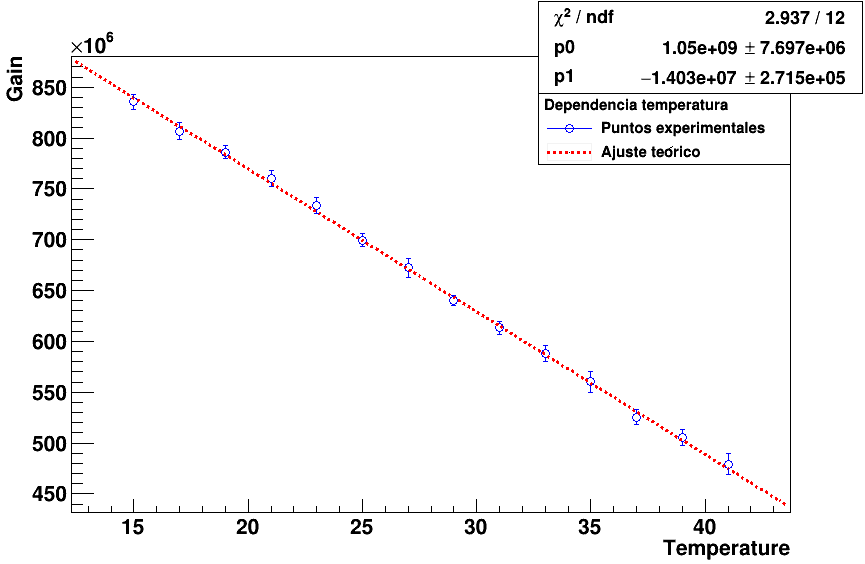
\includegraphics[scale=0.4]{Dependenciatemperatura.png}
\caption{ Ganancia frente a temperatura\label{temperatura}}
\end{figure}

Podemos observar la existencia de un comportamiento lineal casi perfecto en un intervalo de temperatura de $26~\celsius$. Esta es una propiedad que caracteriza al SiPM, una muy buena linealidad en su comportamiento frente a modificaciones en varias magnitudes. Nuevamente comprobamos la calidad del ajuste a partir del test $\chi^2$ obteniendo un valor de $\frac{\chi^2}{ndf}=\frac{2.937}{12}\approx 0.245$, que es un valor relativamente bueno.

En la gráfica~\ref{temperatura} encontramos, como esperábamos~\cite{tesisSiPM}, la existencia de un decrecimiento del valor de la ganancia del SiPM a medida que aumenta la temperatura. Esto es debido a que la zona desierta, que se crea en el SiPM al aplicar un voltaje en inversa y que actúa como zona útil de detección de radiación, depende de la temperatura. En concreto, al aumentar la temperatura estamos incrementando la excitación térmica de los portadores de carga pudiendo, de esta forma, invadir esta zona desierta, reduciéndola su tamaño y, por extensión, la ganancia del SiPM.

La ecuación obtenida en este ajuste $G=aT+b$ toma los siguientes valores: 
\begin{equation}
a=(-140.3 \pm 2.7) \cdot 10^5~\celsius^{-1}
\label{ajustependientetemperatura}
\end{equation}
\begin{equation}
b=(1050.0 \pm 7.7) \cdot 10^6
\label{ajusteordenadatemperatura}
\end{equation}


Esta es un resultado importante, no por el valor numérico, sino porque será la base que utilizaremos para conseguir la compensación de la ganancia.
\end{itemize}

	%\section{Automatic polishing machine for scintillator fiber}\label{sec:PolishingMachine}
	%%De forma totalmente análoga procedemos a determinar la ganancia del SiPM en función de su voltaje operacional. Para ello, realizaremos una serie de medidas a distintos voltajes operacionales y, para cada uno de ellos, calcularemos la ganancia mediante el método expuesto anteriormente. 

Nos centraremos en el rango de voltajes entre el voltaje de ruptura, $V_{BD}= 50.97~\volt$, que es el mínimo voltaje en valor absoluto a partir del cual nos encontramos en modo Geiger y $V_{BD}+5~\volt$, que es un intervalo suficiente para compensar la ganancia en el intervalo de temperaturas que hemos medido. Realizaremos pasos de $0.2~\volt$ entre cada medida realizando un total de $25$ medidas. De nuevo, únicamente realizaremos medidas de $15000$ eventos, suficiente para obtener un espectro  suave.

Para automatizar este proceso procedemos a desarrollar una macro en ROOT que realice este ajuste. Análogamente esta macro poseerá dos partes:
\begin{itemize}
\item{} Por un lado posee un bucle en el que, en cada paso, abre el fichero correspondiente a un voltaje operacional, empezando por el mínimo ($V_{op}=V_{BD}$) realiza todo el estudio anterior y guarda ganancia y voltaje operacional con sus errores en 4 vectores respectivamente. En cada paso aumenta $0.2~\volt$ el voltaje operacional y pasa a leer el siguiente fichero. 
En este estudio, a diferencia del estudio de la temperatura, la incertidumbre en el voltaje viene dada por la precisión del electrómetro (del orden de $1~\milli\volt$) ya que el valor era perfectamente estable. Esta incertidumbre es  totalmente inapreciable tanto a nivel visual en la gráfica como a nivel de variación de la ganancia. 
Hay que tener en cuenta que el voltaje operacional posee un error relativo, definido como $\frac{\sigma_x}{x}$ muy inferior al de la temperatura, siendo estos aproximadamente $0.001\%$ y $0.8\%$ para el voltaje y la temperatura respectivamente. Es decir, las medidas tomadas en este estudio serán más precisas.

\item {} Por otro lado, partiendo de estos $4$ vectores de dimensión $25$ en nuestro caso (igual al número de ficheros que ha leído) que contienen ganancia, temperatura y sus errores de forma ordenada, realiza un ajuste lineal. El ajuste obtenido se presenta en la figura~\ref{voltaje}.

\begin{figure}[hbtp]
\centering
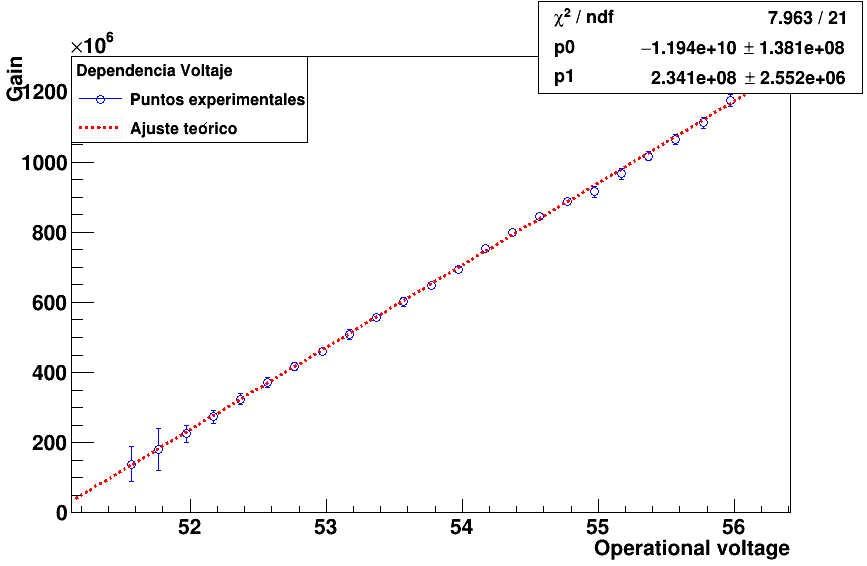
\includegraphics[scale=0.4]{Dependenciavoltaje.png}
\caption{ Ganancia frente a voltaje operacional\label{voltaje}}
\end{figure}

Podemos apreciar de nuevo, como esperábamos~\cite{tesisSiPM}, la existencia de un comportamiento  lineal casi perfecto en un intervalo de voltaje de $5~\volt$. En la gráfica podemos notar la existencia de un mayor error en las medidas de voltajes mas bajos (en valor absoluto). Esto es debido a que nos estamos acercando al voltaje de ruptura, donde el silicio entra en modo Geiger y el valor de la ganancia empieza a ser distinto de cero. Podemos achacar este mayor error a que a estos voltajes, cercanos a la frontera de cambio de comportamiento, el SiPM todavía no funciona de forma adecuada,  pues no funciona todavía en  modo Geiger. Hay que tener en cuenta además que sólo se llegó hasta el voltaje $V_{op}=51,57~\volt$  debido a que, cuando estamos a valores muy cercanos al voltaje de ruptura,  la ganancia sufre una disminución exponencial, siendo imposible realizar su medida.

De nuevo comprobamos la calidad del ajuste a partir del test $\chi^2$, obteniendo un valor de $\frac{\chi^2}{ndf}=\frac{7.963}{21}\approx 0.379$, que indica un ajuste bueno de los datos.

Podemos observar que, al contrario de lo que ocurría con la temperatura, el valor de la ganancia del SiPM aumenta a medida que aumenta el voltaje operacional. Esto es debido a que a medida que aumentamos el voltaje operacional, aumenta la diferencia de potencial en la zona desierta. De esta forma, por un lado, aumentando la zona desierta, por lo que los pares electrón-hueco dispondrán de mayor espacio para generar una avalancha mayor  y, por otro lado, estamos aplicando una mayor tensión sobre los pares electrón-hueco generados al detectar radiación que,  en consecuencia, sufrirán una mayor aceleración. Debido a ello, dispondrán de una mayor energía para producir un mayor número de pares electrón-hueco. En resumen ambos procesos contribuyen a aumentar la ganancia del SiPM.

La ecuación obtenida en este ajuste $G=cV_{op}+d$ toma los siguientes valores: 
\begin{equation}
c=(234.1 \pm 2.6) \cdot 10^6~\volt^{-1}
\label{ajustependientevoltaje}
\end{equation}
\begin{equation}
d=(-119.4 \pm 1.4) \cdot 10^8
\label{ajusteordenadavoltaje}
\end{equation}

Remarquemos de nuevo la importancia de este resultado, ya que es la parte que nos faltaba para poder calcular la compensación de la ganancia.
Además, a modo de comprobación, podemos obtener el voltaje de ruptura a partir de esta expresión, que corresponde al voltaje al cual la ganancia es cero (voltaje a partir del cual estamos en modo Geiger y la ganancia empieza a ser no nula). El voltaje calculado es: 
\begin{equation}
G=0=c \cdot V_{BD} +d \longrightarrow V_{BD}=-\frac{d}{c}=50.99 \pm 0.81~\volt
\label{ajustebdv}
\end{equation}

Vemos que este se acerca de forma extraordinaria al voltaje teórico especificado por Hamamatsu Photonics, $50.97~\volt$.
\end{itemize}
	
	%\section{Splicing machine for scintillator fiber}\label{sec:SplicingMachine}
	%%De forma totalmente análoga procedemos a determinar la ganancia del SiPM en función de su voltaje operacional. Para ello, realizaremos una serie de medidas a distintos voltajes operacionales y, para cada uno de ellos, calcularemos la ganancia mediante el método expuesto anteriormente. 

Nos centraremos en el rango de voltajes entre el voltaje de ruptura, $V_{BD}= 50.97~\volt$, que es el mínimo voltaje en valor absoluto a partir del cual nos encontramos en modo Geiger y $V_{BD}+5~\volt$, que es un intervalo suficiente para compensar la ganancia en el intervalo de temperaturas que hemos medido. Realizaremos pasos de $0.2~\volt$ entre cada medida realizando un total de $25$ medidas. De nuevo, únicamente realizaremos medidas de $15000$ eventos, suficiente para obtener un espectro  suave.

Para automatizar este proceso procedemos a desarrollar una macro en ROOT que realice este ajuste. Análogamente esta macro poseerá dos partes:
\begin{itemize}
\item{} Por un lado posee un bucle en el que, en cada paso, abre el fichero correspondiente a un voltaje operacional, empezando por el mínimo ($V_{op}=V_{BD}$) realiza todo el estudio anterior y guarda ganancia y voltaje operacional con sus errores en 4 vectores respectivamente. En cada paso aumenta $0.2~\volt$ el voltaje operacional y pasa a leer el siguiente fichero. 
En este estudio, a diferencia del estudio de la temperatura, la incertidumbre en el voltaje viene dada por la precisión del electrómetro (del orden de $1~\milli\volt$) ya que el valor era perfectamente estable. Esta incertidumbre es  totalmente inapreciable tanto a nivel visual en la gráfica como a nivel de variación de la ganancia. 
Hay que tener en cuenta que el voltaje operacional posee un error relativo, definido como $\frac{\sigma_x}{x}$ muy inferior al de la temperatura, siendo estos aproximadamente $0.001\%$ y $0.8\%$ para el voltaje y la temperatura respectivamente. Es decir, las medidas tomadas en este estudio serán más precisas.

\item {} Por otro lado, partiendo de estos $4$ vectores de dimensión $25$ en nuestro caso (igual al número de ficheros que ha leído) que contienen ganancia, temperatura y sus errores de forma ordenada, realiza un ajuste lineal. El ajuste obtenido se presenta en la figura~\ref{voltaje}.

\begin{figure}[hbtp]
\centering
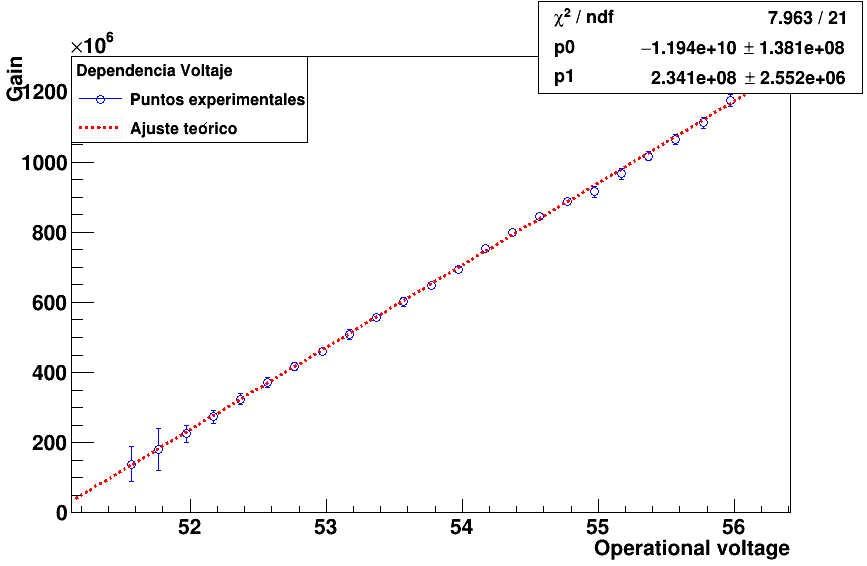
\includegraphics[scale=0.4]{Dependenciavoltaje.png}
\caption{ Ganancia frente a voltaje operacional\label{voltaje}}
\end{figure}

Podemos apreciar de nuevo, como esperábamos~\cite{tesisSiPM}, la existencia de un comportamiento  lineal casi perfecto en un intervalo de voltaje de $5~\volt$. En la gráfica podemos notar la existencia de un mayor error en las medidas de voltajes mas bajos (en valor absoluto). Esto es debido a que nos estamos acercando al voltaje de ruptura, donde el silicio entra en modo Geiger y el valor de la ganancia empieza a ser distinto de cero. Podemos achacar este mayor error a que a estos voltajes, cercanos a la frontera de cambio de comportamiento, el SiPM todavía no funciona de forma adecuada,  pues no funciona todavía en  modo Geiger. Hay que tener en cuenta además que sólo se llegó hasta el voltaje $V_{op}=51,57~\volt$  debido a que, cuando estamos a valores muy cercanos al voltaje de ruptura,  la ganancia sufre una disminución exponencial, siendo imposible realizar su medida.

De nuevo comprobamos la calidad del ajuste a partir del test $\chi^2$, obteniendo un valor de $\frac{\chi^2}{ndf}=\frac{7.963}{21}\approx 0.379$, que indica un ajuste bueno de los datos.

Podemos observar que, al contrario de lo que ocurría con la temperatura, el valor de la ganancia del SiPM aumenta a medida que aumenta el voltaje operacional. Esto es debido a que a medida que aumentamos el voltaje operacional, aumenta la diferencia de potencial en la zona desierta. De esta forma, por un lado, aumentando la zona desierta, por lo que los pares electrón-hueco dispondrán de mayor espacio para generar una avalancha mayor  y, por otro lado, estamos aplicando una mayor tensión sobre los pares electrón-hueco generados al detectar radiación que,  en consecuencia, sufrirán una mayor aceleración. Debido a ello, dispondrán de una mayor energía para producir un mayor número de pares electrón-hueco. En resumen ambos procesos contribuyen a aumentar la ganancia del SiPM.

La ecuación obtenida en este ajuste $G=cV_{op}+d$ toma los siguientes valores: 
\begin{equation}
c=(234.1 \pm 2.6) \cdot 10^6~\volt^{-1}
\label{ajustependientevoltaje}
\end{equation}
\begin{equation}
d=(-119.4 \pm 1.4) \cdot 10^8
\label{ajusteordenadavoltaje}
\end{equation}

Remarquemos de nuevo la importancia de este resultado, ya que es la parte que nos faltaba para poder calcular la compensación de la ganancia.
Además, a modo de comprobación, podemos obtener el voltaje de ruptura a partir de esta expresión, que corresponde al voltaje al cual la ganancia es cero (voltaje a partir del cual estamos en modo Geiger y la ganancia empieza a ser no nula). El voltaje calculado es: 
\begin{equation}
G=0=c \cdot V_{BD} +d \longrightarrow V_{BD}=-\frac{d}{c}=50.99 \pm 0.81~\volt
\label{ajustebdv}
\end{equation}

Vemos que este se acerca de forma extraordinaria al voltaje teórico especificado por Hamamatsu Photonics, $50.97~\volt$.
\end{itemize}
	
	%DE aquí para abajo todos los estudios realizados con fibras...
	%\section{Estabilización de la ganancia}\label{sec:Compensacion}
	%%Finalmente, con toda la información obtenida en los apartados anteriores, procedemos a desarrollar un protocolo de compensación de la variación de la ganancia debido a la temperatura. Nuestro objetivo es que, ante una modificación de la ganancia debida a una variación de la temperatura ambiente (por ejemplo debido a variaciones climatológicas) aplicar una variación adecuada en el voltaje operacional que devuelva a la ganancia a su valor inicial.

Como ya se ha explicado anteriormente, la importancia de este estudio de compensación radica en que deseamos utilizar el detector  a modo de alarma. Dado que este estará expuesto a condiciones climáticas arbitrarias, inevitablemente sufrirá variaciones de temperatura. Si queremos que el detector final sea capaz de avisar en caso de obtener una señal demasiado grande y que esta señal se corresponda a una fuga de tritio, necesitamos que el sistema posea una ganancia constante.

Las expresiones que se han obtenido con las dos calibraciones anteriores son:
\begin{equation}
G(V_{op})=cV_{op}+d; \qquad G(T)=aT+b
\label{gananciatotal}
\end{equation}

Esto implica que una variación de la ganancia en cada una de estas magnitudes viene dada como:
\begin{equation}
\partial G(V_{op}) = c \partial V_{op}; \qquad \partial G(T) = a \partial T
\label{variacionparcialganancia}
\end{equation}

Finalmente, la variación total de la ganancia ante una variación de ambas magnitudes viene dada por:
\begin{equation}
\partial G_{tot} = \partial G(V_{op}) + \partial G(T)
\label{variaciontotalganancia}
\end{equation}

Por tanto, si queremos que el valor de la ganancia se conserve ante una variación de ambas magnitudes, tenemos que conseguir que: 
\begin{equation}
\partial G_{tot} = 0 =  \partial G(V_{op}) + \partial G(T) \longrightarrow \partial G(V_{op}) = -\partial G(T)  
\label{basecompensacion}
\end{equation}
En otras palabras, debemos producir una  variación opuesta  de la ganancia con la modificación del voltaje a la que se ha producido al variar la temperatura. Para determinar esta variación, únicamente sustituimos las expresiones anteriormente obtenidas para cada diferencial de la ganancia:
\begin{equation}
\partial G(V_{op}) = - \partial G(T)  \longrightarrow c \partial V_{op}= - a \partial T \longrightarrow  \partial V_{op}= - \frac{a}{c} \partial T
\label{compensacionparciales}
\end{equation}
En trabajos anteriores\cite{TFMSiPM2, tesisSiPM, cladtesis} se ha visto que ambas pendientes, $a$ y $c$, apenas varían en voltaje y temperatura. Por tanto, en primera aproximación, podemos considerarlas constantes en ambas magnitudes. Con ello integramos a cada lado y obtenemos:
\begin{equation}
\int_{V_i}^{V_f} \partial V_{op}= - \frac{a}{c} \int_{T_i}^{T_f}\partial T = - \frac{a}{c} \Delta T \longrightarrow \Delta V_{op}= e \Delta T
\label{integral}
\end{equation}
donde se ha introducido un nuevo parámetro: $$e=-\frac{a}{c}$$ cuyo valor se obtiene de las ecuaciones $\eqref{ajustependientetemperatura}$  y $\eqref{ajustependientevoltaje}$:
\begin{equation}
c=(234.1 \pm 2.6) \cdot 10^6~\volt^{-1}
\label{pendientevoltaje}
\end{equation}
\begin{equation}
a=(-140.3 \pm 2.7) \cdot 10^5~ \celsius^{-1}
\label{pendientetemperatura}
\end{equation}
\begin{equation}
e=-\frac{a}{c} = 59.9 \pm 1.3 ~\milli\volt  \celsius^{-1}
\label{pendientecompensacion}
\end{equation}
donde el error de $e$ se ha obtenido mediante propagación de errores. 

Finalmente, procedemos a analizar el resultado. Hemos obtenido dos dependencias de la ganancia lineales y opuestas. Por un lado la ganancia disminuye con la temperatura y por otro lado la ganancia aumenta con el voltaje operacional. Por tanto, si queremos conseguir modificaciones opuestas de la ganancia debemos desplazar voltaje y temperatura en la misma dirección (aumentar o disminuir ambas magnitudes simultáneamente). Si analizamos el resultado vemos que, efectivamente, tenemos una dependencia positiva.
También apreciamos que obtenemos un valor dos órdenes de magnitud inferior a la unidad. Esto es debido a que la dependencia de la ganancia con el voltaje es mucho más marcada que la variación con la temperatura (mayor pendiente en valor absoluto para el ajuste del voltaje que para el ajuste de la temperatura). Este es el motivo por el que se toma pasos más reducidos para el voltaje que para la temperatura. 

En resumen, la ecuación que nos dicta cual es la variación que debemos aplicar al voltaje para mantener un valor de ganancia constante (compensar la ganancia) ante una variación de la temperatura conocida (que puede ser medida con un sensor de temperatura) es:
\begin{equation}
\Delta V_{op}=0.060 \cdot \Delta T \longrightarrow V_1-V_{ref}=0.060(T_1-T_{ref})
\label{compensacionfinal}
\end{equation}
Donde $V_1$ es el voltaje con el que hay que alimentar al SiPM a una temperatura ambiental de $T_1$ para mantener la ganancia constante a su valor de referencia. Para realizar este cálculo, se necesita tomar un valor de voltaje operacional y temperatura como referencía, cuya ganancia es la que mantendremos. Para estos valores de referencia elegiremos el caso anteriormente mostrado en la sección de análisis de datos correspondiente a temperatura $25~\celsius$, humedad del $45\% $ y voltaje operacional de $53.97~\volt = V_{BD}+ 3~\volt$ , cuya ganancia total hemos visto que corresponde a $7.18 \cdot 10^8$. Por tanto, el valor de voltaje operacional $V_1$ con el que hay que alimentar un SiPM a temperatura $T_1$, para mantener una ganancia de $7.18 \cdot 10^8$ es:
\begin{equation}
V_1=0.060T_1+52.47
\label{compensacionfinal}
\end{equation}




Procedemos a realizar una verificación midiendo los casos de $21, 23, 25, 27$ y  $29~\celsius$. En cada uno de ellos se corregirá el voltaje de alimentación de forma adecuada para mantener el mismo valor de la ganancia. El valor de la ganancia medida para cada caso se muestra en la figura~\ref{compensacion}. 

\begin{figure}[hbtp]
\centering
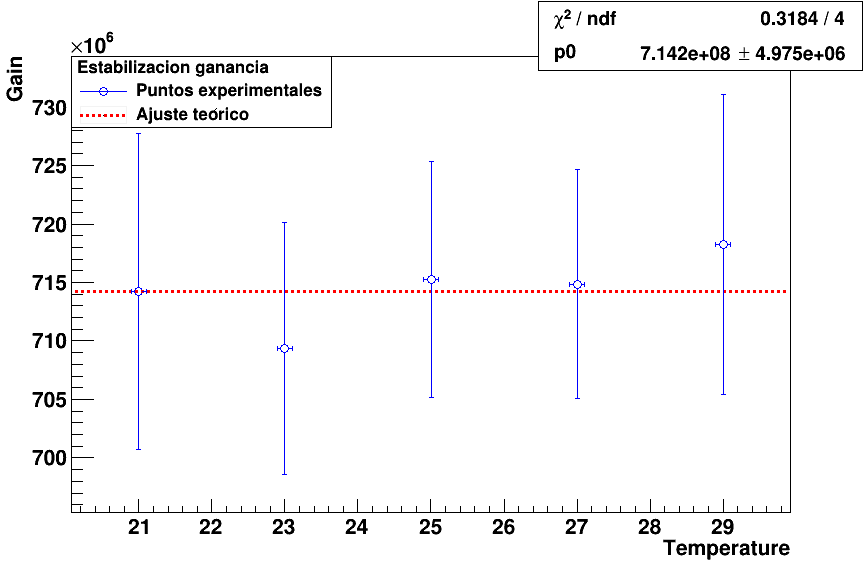
\includegraphics[scale=0.4]{compensacion.png}
\caption{Ganancia frente a temperatura después de corregir con el voltaje de operacion.\label{compensacion}}
\end{figure}
donde la raya roja corresponde al ajuste a una constante. Su valor, correspondiente al valor de la ganancia es $G=(714.2 \pm 4.9) \cdot 10^6$. Comprobamos la calidad del ajuste a partir del test $\chi^2$ obteniendo un valor de $\frac{\chi^2}{ndf}=\frac{0.318}{4}\approx 0.0795$, valor ligeramente bajo, probablemente debido a una sobreestimación de los errores (algo que ya puede apreciarse en la imagen).

Vemos que el método funciona de manera muy eficaz, ya que la ganancia presenta variaciones muy pequeñas de aproximadamente $\Delta G=5 \cdot 10^6$, que corresponde a una variación relativa de $\sigma_{rel}=0.28\%$. Hemos comprobado por tanto que se trata de un método realmente eficaz.

La máxima variación se observó a $23~\celsius$, debido a que fue una medida realizada muchas horas después de tomarse las otras y existen factores externos que no podemos controlar que afectan al sistema. En este tiempo más largo transcurrido es más probable que hayan cambiado estos factores. Sin embargo, puede observarse en todo momento que la variación de la ganancia es mínima verificando en gran medida la ecuación anteriormente obtenida.



%\chapter{Photomultiplier tubes (PMTs)} \label{sec:PMT}
%\input{./Sections/4Fibras}
	%\section{Introduction}\label{sec:IntroductionPMTs}
	%%De forma totalmente análoga procedemos a determinar la ganancia del SiPM en función de su voltaje operacional. Para ello, realizaremos una serie de medidas a distintos voltajes operacionales y, para cada uno de ellos, calcularemos la ganancia mediante el método expuesto anteriormente. 

Nos centraremos en el rango de voltajes entre el voltaje de ruptura, $V_{BD}= 50.97~\volt$, que es el mínimo voltaje en valor absoluto a partir del cual nos encontramos en modo Geiger y $V_{BD}+5~\volt$, que es un intervalo suficiente para compensar la ganancia en el intervalo de temperaturas que hemos medido. Realizaremos pasos de $0.2~\volt$ entre cada medida realizando un total de $25$ medidas. De nuevo, únicamente realizaremos medidas de $15000$ eventos, suficiente para obtener un espectro  suave.

Para automatizar este proceso procedemos a desarrollar una macro en ROOT que realice este ajuste. Análogamente esta macro poseerá dos partes:
\begin{itemize}
\item{} Por un lado posee un bucle en el que, en cada paso, abre el fichero correspondiente a un voltaje operacional, empezando por el mínimo ($V_{op}=V_{BD}$) realiza todo el estudio anterior y guarda ganancia y voltaje operacional con sus errores en 4 vectores respectivamente. En cada paso aumenta $0.2~\volt$ el voltaje operacional y pasa a leer el siguiente fichero. 
En este estudio, a diferencia del estudio de la temperatura, la incertidumbre en el voltaje viene dada por la precisión del electrómetro (del orden de $1~\milli\volt$) ya que el valor era perfectamente estable. Esta incertidumbre es  totalmente inapreciable tanto a nivel visual en la gráfica como a nivel de variación de la ganancia. 
Hay que tener en cuenta que el voltaje operacional posee un error relativo, definido como $\frac{\sigma_x}{x}$ muy inferior al de la temperatura, siendo estos aproximadamente $0.001\%$ y $0.8\%$ para el voltaje y la temperatura respectivamente. Es decir, las medidas tomadas en este estudio serán más precisas.

\item {} Por otro lado, partiendo de estos $4$ vectores de dimensión $25$ en nuestro caso (igual al número de ficheros que ha leído) que contienen ganancia, temperatura y sus errores de forma ordenada, realiza un ajuste lineal. El ajuste obtenido se presenta en la figura~\ref{voltaje}.

\begin{figure}[hbtp]
\centering
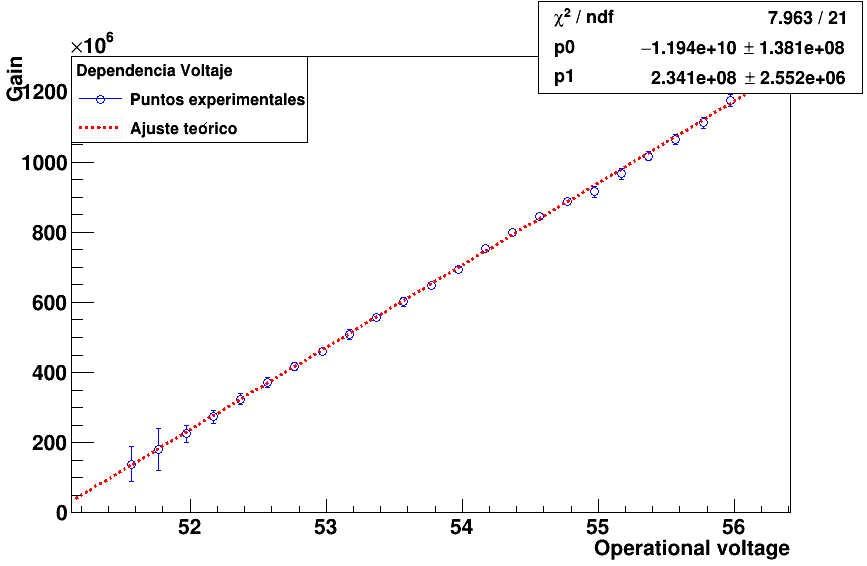
\includegraphics[scale=0.4]{Dependenciavoltaje.png}
\caption{ Ganancia frente a voltaje operacional\label{voltaje}}
\end{figure}

Podemos apreciar de nuevo, como esperábamos~\cite{tesisSiPM}, la existencia de un comportamiento  lineal casi perfecto en un intervalo de voltaje de $5~\volt$. En la gráfica podemos notar la existencia de un mayor error en las medidas de voltajes mas bajos (en valor absoluto). Esto es debido a que nos estamos acercando al voltaje de ruptura, donde el silicio entra en modo Geiger y el valor de la ganancia empieza a ser distinto de cero. Podemos achacar este mayor error a que a estos voltajes, cercanos a la frontera de cambio de comportamiento, el SiPM todavía no funciona de forma adecuada,  pues no funciona todavía en  modo Geiger. Hay que tener en cuenta además que sólo se llegó hasta el voltaje $V_{op}=51,57~\volt$  debido a que, cuando estamos a valores muy cercanos al voltaje de ruptura,  la ganancia sufre una disminución exponencial, siendo imposible realizar su medida.

De nuevo comprobamos la calidad del ajuste a partir del test $\chi^2$, obteniendo un valor de $\frac{\chi^2}{ndf}=\frac{7.963}{21}\approx 0.379$, que indica un ajuste bueno de los datos.

Podemos observar que, al contrario de lo que ocurría con la temperatura, el valor de la ganancia del SiPM aumenta a medida que aumenta el voltaje operacional. Esto es debido a que a medida que aumentamos el voltaje operacional, aumenta la diferencia de potencial en la zona desierta. De esta forma, por un lado, aumentando la zona desierta, por lo que los pares electrón-hueco dispondrán de mayor espacio para generar una avalancha mayor  y, por otro lado, estamos aplicando una mayor tensión sobre los pares electrón-hueco generados al detectar radiación que,  en consecuencia, sufrirán una mayor aceleración. Debido a ello, dispondrán de una mayor energía para producir un mayor número de pares electrón-hueco. En resumen ambos procesos contribuyen a aumentar la ganancia del SiPM.

La ecuación obtenida en este ajuste $G=cV_{op}+d$ toma los siguientes valores: 
\begin{equation}
c=(234.1 \pm 2.6) \cdot 10^6~\volt^{-1}
\label{ajustependientevoltaje}
\end{equation}
\begin{equation}
d=(-119.4 \pm 1.4) \cdot 10^8
\label{ajusteordenadavoltaje}
\end{equation}

Remarquemos de nuevo la importancia de este resultado, ya que es la parte que nos faltaba para poder calcular la compensación de la ganancia.
Además, a modo de comprobación, podemos obtener el voltaje de ruptura a partir de esta expresión, que corresponde al voltaje al cual la ganancia es cero (voltaje a partir del cual estamos en modo Geiger y la ganancia empieza a ser no nula). El voltaje calculado es: 
\begin{equation}
G=0=c \cdot V_{BD} +d \longrightarrow V_{BD}=-\frac{d}{c}=50.99 \pm 0.81~\volt
\label{ajustebdv}
\end{equation}

Vemos que este se acerca de forma extraordinaria al voltaje teórico especificado por Hamamatsu Photonics, $50.97~\volt$.
\end{itemize}
	
	%\section{Calibration of the PMTs}\label{sec:CalibrationPMTs}
	%%De forma totalmente análoga procedemos a determinar la ganancia del SiPM en función de su voltaje operacional. Para ello, realizaremos una serie de medidas a distintos voltajes operacionales y, para cada uno de ellos, calcularemos la ganancia mediante el método expuesto anteriormente. 

Nos centraremos en el rango de voltajes entre el voltaje de ruptura, $V_{BD}= 50.97~\volt$, que es el mínimo voltaje en valor absoluto a partir del cual nos encontramos en modo Geiger y $V_{BD}+5~\volt$, que es un intervalo suficiente para compensar la ganancia en el intervalo de temperaturas que hemos medido. Realizaremos pasos de $0.2~\volt$ entre cada medida realizando un total de $25$ medidas. De nuevo, únicamente realizaremos medidas de $15000$ eventos, suficiente para obtener un espectro  suave.

Para automatizar este proceso procedemos a desarrollar una macro en ROOT que realice este ajuste. Análogamente esta macro poseerá dos partes:
\begin{itemize}
\item{} Por un lado posee un bucle en el que, en cada paso, abre el fichero correspondiente a un voltaje operacional, empezando por el mínimo ($V_{op}=V_{BD}$) realiza todo el estudio anterior y guarda ganancia y voltaje operacional con sus errores en 4 vectores respectivamente. En cada paso aumenta $0.2~\volt$ el voltaje operacional y pasa a leer el siguiente fichero. 
En este estudio, a diferencia del estudio de la temperatura, la incertidumbre en el voltaje viene dada por la precisión del electrómetro (del orden de $1~\milli\volt$) ya que el valor era perfectamente estable. Esta incertidumbre es  totalmente inapreciable tanto a nivel visual en la gráfica como a nivel de variación de la ganancia. 
Hay que tener en cuenta que el voltaje operacional posee un error relativo, definido como $\frac{\sigma_x}{x}$ muy inferior al de la temperatura, siendo estos aproximadamente $0.001\%$ y $0.8\%$ para el voltaje y la temperatura respectivamente. Es decir, las medidas tomadas en este estudio serán más precisas.

\item {} Por otro lado, partiendo de estos $4$ vectores de dimensión $25$ en nuestro caso (igual al número de ficheros que ha leído) que contienen ganancia, temperatura y sus errores de forma ordenada, realiza un ajuste lineal. El ajuste obtenido se presenta en la figura~\ref{voltaje}.

\begin{figure}[hbtp]
\centering
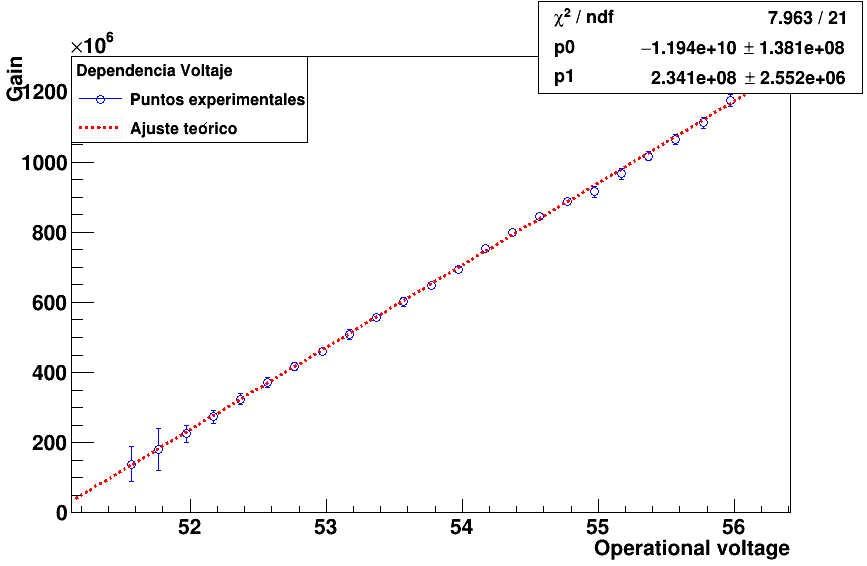
\includegraphics[scale=0.4]{Dependenciavoltaje.png}
\caption{ Ganancia frente a voltaje operacional\label{voltaje}}
\end{figure}

Podemos apreciar de nuevo, como esperábamos~\cite{tesisSiPM}, la existencia de un comportamiento  lineal casi perfecto en un intervalo de voltaje de $5~\volt$. En la gráfica podemos notar la existencia de un mayor error en las medidas de voltajes mas bajos (en valor absoluto). Esto es debido a que nos estamos acercando al voltaje de ruptura, donde el silicio entra en modo Geiger y el valor de la ganancia empieza a ser distinto de cero. Podemos achacar este mayor error a que a estos voltajes, cercanos a la frontera de cambio de comportamiento, el SiPM todavía no funciona de forma adecuada,  pues no funciona todavía en  modo Geiger. Hay que tener en cuenta además que sólo se llegó hasta el voltaje $V_{op}=51,57~\volt$  debido a que, cuando estamos a valores muy cercanos al voltaje de ruptura,  la ganancia sufre una disminución exponencial, siendo imposible realizar su medida.

De nuevo comprobamos la calidad del ajuste a partir del test $\chi^2$, obteniendo un valor de $\frac{\chi^2}{ndf}=\frac{7.963}{21}\approx 0.379$, que indica un ajuste bueno de los datos.

Podemos observar que, al contrario de lo que ocurría con la temperatura, el valor de la ganancia del SiPM aumenta a medida que aumenta el voltaje operacional. Esto es debido a que a medida que aumentamos el voltaje operacional, aumenta la diferencia de potencial en la zona desierta. De esta forma, por un lado, aumentando la zona desierta, por lo que los pares electrón-hueco dispondrán de mayor espacio para generar una avalancha mayor  y, por otro lado, estamos aplicando una mayor tensión sobre los pares electrón-hueco generados al detectar radiación que,  en consecuencia, sufrirán una mayor aceleración. Debido a ello, dispondrán de una mayor energía para producir un mayor número de pares electrón-hueco. En resumen ambos procesos contribuyen a aumentar la ganancia del SiPM.

La ecuación obtenida en este ajuste $G=cV_{op}+d$ toma los siguientes valores: 
\begin{equation}
c=(234.1 \pm 2.6) \cdot 10^6~\volt^{-1}
\label{ajustependientevoltaje}
\end{equation}
\begin{equation}
d=(-119.4 \pm 1.4) \cdot 10^8
\label{ajusteordenadavoltaje}
\end{equation}

Remarquemos de nuevo la importancia de este resultado, ya que es la parte que nos faltaba para poder calcular la compensación de la ganancia.
Además, a modo de comprobación, podemos obtener el voltaje de ruptura a partir de esta expresión, que corresponde al voltaje al cual la ganancia es cero (voltaje a partir del cual estamos en modo Geiger y la ganancia empieza a ser no nula). El voltaje calculado es: 
\begin{equation}
G=0=c \cdot V_{BD} +d \longrightarrow V_{BD}=-\frac{d}{c}=50.99 \pm 0.81~\volt
\label{ajustebdv}
\end{equation}

Vemos que este se acerca de forma extraordinaria al voltaje teórico especificado por Hamamatsu Photonics, $50.97~\volt$.
\end{itemize}
	
	%\subsection{Gain calibration of the PMTs}\label{sec:GainCalibrationPMTs}
	%%De forma totalmente análoga procedemos a determinar la ganancia del SiPM en función de su voltaje operacional. Para ello, realizaremos una serie de medidas a distintos voltajes operacionales y, para cada uno de ellos, calcularemos la ganancia mediante el método expuesto anteriormente. 

Nos centraremos en el rango de voltajes entre el voltaje de ruptura, $V_{BD}= 50.97~\volt$, que es el mínimo voltaje en valor absoluto a partir del cual nos encontramos en modo Geiger y $V_{BD}+5~\volt$, que es un intervalo suficiente para compensar la ganancia en el intervalo de temperaturas que hemos medido. Realizaremos pasos de $0.2~\volt$ entre cada medida realizando un total de $25$ medidas. De nuevo, únicamente realizaremos medidas de $15000$ eventos, suficiente para obtener un espectro  suave.

Para automatizar este proceso procedemos a desarrollar una macro en ROOT que realice este ajuste. Análogamente esta macro poseerá dos partes:
\begin{itemize}
\item{} Por un lado posee un bucle en el que, en cada paso, abre el fichero correspondiente a un voltaje operacional, empezando por el mínimo ($V_{op}=V_{BD}$) realiza todo el estudio anterior y guarda ganancia y voltaje operacional con sus errores en 4 vectores respectivamente. En cada paso aumenta $0.2~\volt$ el voltaje operacional y pasa a leer el siguiente fichero. 
En este estudio, a diferencia del estudio de la temperatura, la incertidumbre en el voltaje viene dada por la precisión del electrómetro (del orden de $1~\milli\volt$) ya que el valor era perfectamente estable. Esta incertidumbre es  totalmente inapreciable tanto a nivel visual en la gráfica como a nivel de variación de la ganancia. 
Hay que tener en cuenta que el voltaje operacional posee un error relativo, definido como $\frac{\sigma_x}{x}$ muy inferior al de la temperatura, siendo estos aproximadamente $0.001\%$ y $0.8\%$ para el voltaje y la temperatura respectivamente. Es decir, las medidas tomadas en este estudio serán más precisas.

\item {} Por otro lado, partiendo de estos $4$ vectores de dimensión $25$ en nuestro caso (igual al número de ficheros que ha leído) que contienen ganancia, temperatura y sus errores de forma ordenada, realiza un ajuste lineal. El ajuste obtenido se presenta en la figura~\ref{voltaje}.

\begin{figure}[hbtp]
\centering
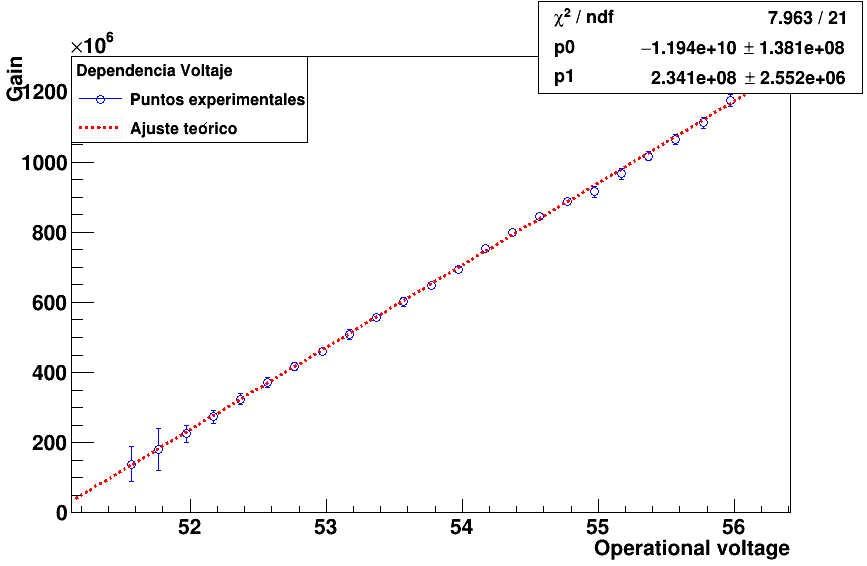
\includegraphics[scale=0.4]{Dependenciavoltaje.png}
\caption{ Ganancia frente a voltaje operacional\label{voltaje}}
\end{figure}

Podemos apreciar de nuevo, como esperábamos~\cite{tesisSiPM}, la existencia de un comportamiento  lineal casi perfecto en un intervalo de voltaje de $5~\volt$. En la gráfica podemos notar la existencia de un mayor error en las medidas de voltajes mas bajos (en valor absoluto). Esto es debido a que nos estamos acercando al voltaje de ruptura, donde el silicio entra en modo Geiger y el valor de la ganancia empieza a ser distinto de cero. Podemos achacar este mayor error a que a estos voltajes, cercanos a la frontera de cambio de comportamiento, el SiPM todavía no funciona de forma adecuada,  pues no funciona todavía en  modo Geiger. Hay que tener en cuenta además que sólo se llegó hasta el voltaje $V_{op}=51,57~\volt$  debido a que, cuando estamos a valores muy cercanos al voltaje de ruptura,  la ganancia sufre una disminución exponencial, siendo imposible realizar su medida.

De nuevo comprobamos la calidad del ajuste a partir del test $\chi^2$, obteniendo un valor de $\frac{\chi^2}{ndf}=\frac{7.963}{21}\approx 0.379$, que indica un ajuste bueno de los datos.

Podemos observar que, al contrario de lo que ocurría con la temperatura, el valor de la ganancia del SiPM aumenta a medida que aumenta el voltaje operacional. Esto es debido a que a medida que aumentamos el voltaje operacional, aumenta la diferencia de potencial en la zona desierta. De esta forma, por un lado, aumentando la zona desierta, por lo que los pares electrón-hueco dispondrán de mayor espacio para generar una avalancha mayor  y, por otro lado, estamos aplicando una mayor tensión sobre los pares electrón-hueco generados al detectar radiación que,  en consecuencia, sufrirán una mayor aceleración. Debido a ello, dispondrán de una mayor energía para producir un mayor número de pares electrón-hueco. En resumen ambos procesos contribuyen a aumentar la ganancia del SiPM.

La ecuación obtenida en este ajuste $G=cV_{op}+d$ toma los siguientes valores: 
\begin{equation}
c=(234.1 \pm 2.6) \cdot 10^6~\volt^{-1}
\label{ajustependientevoltaje}
\end{equation}
\begin{equation}
d=(-119.4 \pm 1.4) \cdot 10^8
\label{ajusteordenadavoltaje}
\end{equation}

Remarquemos de nuevo la importancia de este resultado, ya que es la parte que nos faltaba para poder calcular la compensación de la ganancia.
Además, a modo de comprobación, podemos obtener el voltaje de ruptura a partir de esta expresión, que corresponde al voltaje al cual la ganancia es cero (voltaje a partir del cual estamos en modo Geiger y la ganancia empieza a ser no nula). El voltaje calculado es: 
\begin{equation}
G=0=c \cdot V_{BD} +d \longrightarrow V_{BD}=-\frac{d}{c}=50.99 \pm 0.81~\volt
\label{ajustebdv}
\end{equation}

Vemos que este se acerca de forma extraordinaria al voltaje teórico especificado por Hamamatsu Photonics, $50.97~\volt$.
\end{itemize}
	
	%\subsection{Aquí para abajo las demas calibraciones que haré con los PMTs}\label{sec:demáscalibraciones}
	%%De forma totalmente análoga procedemos a determinar la ganancia del SiPM en función de su voltaje operacional. Para ello, realizaremos una serie de medidas a distintos voltajes operacionales y, para cada uno de ellos, calcularemos la ganancia mediante el método expuesto anteriormente. 

Nos centraremos en el rango de voltajes entre el voltaje de ruptura, $V_{BD}= 50.97~\volt$, que es el mínimo voltaje en valor absoluto a partir del cual nos encontramos en modo Geiger y $V_{BD}+5~\volt$, que es un intervalo suficiente para compensar la ganancia en el intervalo de temperaturas que hemos medido. Realizaremos pasos de $0.2~\volt$ entre cada medida realizando un total de $25$ medidas. De nuevo, únicamente realizaremos medidas de $15000$ eventos, suficiente para obtener un espectro  suave.

Para automatizar este proceso procedemos a desarrollar una macro en ROOT que realice este ajuste. Análogamente esta macro poseerá dos partes:
\begin{itemize}
\item{} Por un lado posee un bucle en el que, en cada paso, abre el fichero correspondiente a un voltaje operacional, empezando por el mínimo ($V_{op}=V_{BD}$) realiza todo el estudio anterior y guarda ganancia y voltaje operacional con sus errores en 4 vectores respectivamente. En cada paso aumenta $0.2~\volt$ el voltaje operacional y pasa a leer el siguiente fichero. 
En este estudio, a diferencia del estudio de la temperatura, la incertidumbre en el voltaje viene dada por la precisión del electrómetro (del orden de $1~\milli\volt$) ya que el valor era perfectamente estable. Esta incertidumbre es  totalmente inapreciable tanto a nivel visual en la gráfica como a nivel de variación de la ganancia. 
Hay que tener en cuenta que el voltaje operacional posee un error relativo, definido como $\frac{\sigma_x}{x}$ muy inferior al de la temperatura, siendo estos aproximadamente $0.001\%$ y $0.8\%$ para el voltaje y la temperatura respectivamente. Es decir, las medidas tomadas en este estudio serán más precisas.

\item {} Por otro lado, partiendo de estos $4$ vectores de dimensión $25$ en nuestro caso (igual al número de ficheros que ha leído) que contienen ganancia, temperatura y sus errores de forma ordenada, realiza un ajuste lineal. El ajuste obtenido se presenta en la figura~\ref{voltaje}.

\begin{figure}[hbtp]
\centering
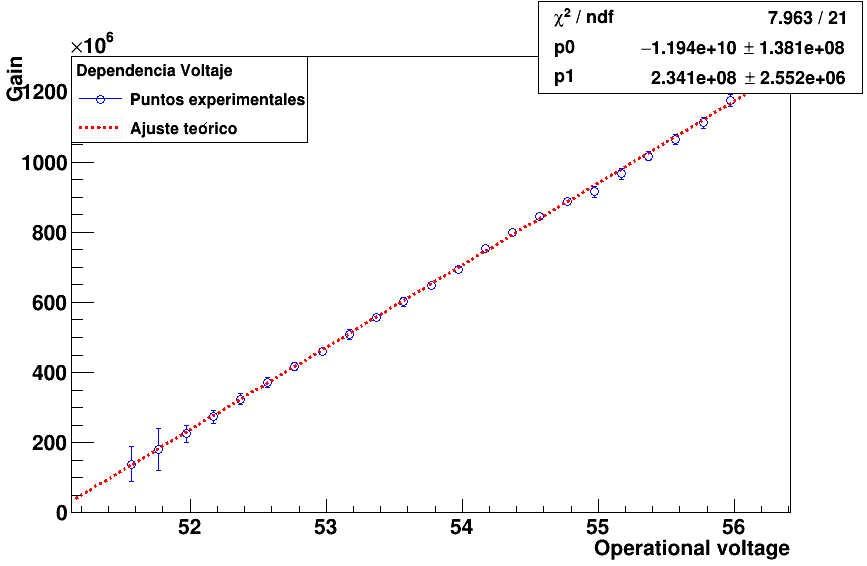
\includegraphics[scale=0.4]{Dependenciavoltaje.png}
\caption{ Ganancia frente a voltaje operacional\label{voltaje}}
\end{figure}

Podemos apreciar de nuevo, como esperábamos~\cite{tesisSiPM}, la existencia de un comportamiento  lineal casi perfecto en un intervalo de voltaje de $5~\volt$. En la gráfica podemos notar la existencia de un mayor error en las medidas de voltajes mas bajos (en valor absoluto). Esto es debido a que nos estamos acercando al voltaje de ruptura, donde el silicio entra en modo Geiger y el valor de la ganancia empieza a ser distinto de cero. Podemos achacar este mayor error a que a estos voltajes, cercanos a la frontera de cambio de comportamiento, el SiPM todavía no funciona de forma adecuada,  pues no funciona todavía en  modo Geiger. Hay que tener en cuenta además que sólo se llegó hasta el voltaje $V_{op}=51,57~\volt$  debido a que, cuando estamos a valores muy cercanos al voltaje de ruptura,  la ganancia sufre una disminución exponencial, siendo imposible realizar su medida.

De nuevo comprobamos la calidad del ajuste a partir del test $\chi^2$, obteniendo un valor de $\frac{\chi^2}{ndf}=\frac{7.963}{21}\approx 0.379$, que indica un ajuste bueno de los datos.

Podemos observar que, al contrario de lo que ocurría con la temperatura, el valor de la ganancia del SiPM aumenta a medida que aumenta el voltaje operacional. Esto es debido a que a medida que aumentamos el voltaje operacional, aumenta la diferencia de potencial en la zona desierta. De esta forma, por un lado, aumentando la zona desierta, por lo que los pares electrón-hueco dispondrán de mayor espacio para generar una avalancha mayor  y, por otro lado, estamos aplicando una mayor tensión sobre los pares electrón-hueco generados al detectar radiación que,  en consecuencia, sufrirán una mayor aceleración. Debido a ello, dispondrán de una mayor energía para producir un mayor número de pares electrón-hueco. En resumen ambos procesos contribuyen a aumentar la ganancia del SiPM.

La ecuación obtenida en este ajuste $G=cV_{op}+d$ toma los siguientes valores: 
\begin{equation}
c=(234.1 \pm 2.6) \cdot 10^6~\volt^{-1}
\label{ajustependientevoltaje}
\end{equation}
\begin{equation}
d=(-119.4 \pm 1.4) \cdot 10^8
\label{ajusteordenadavoltaje}
\end{equation}

Remarquemos de nuevo la importancia de este resultado, ya que es la parte que nos faltaba para poder calcular la compensación de la ganancia.
Además, a modo de comprobación, podemos obtener el voltaje de ruptura a partir de esta expresión, que corresponde al voltaje al cual la ganancia es cero (voltaje a partir del cual estamos en modo Geiger y la ganancia empieza a ser no nula). El voltaje calculado es: 
\begin{equation}
G=0=c \cdot V_{BD} +d \longrightarrow V_{BD}=-\frac{d}{c}=50.99 \pm 0.81~\volt
\label{ajustebdv}
\end{equation}

Vemos que este se acerca de forma extraordinaria al voltaje teórico especificado por Hamamatsu Photonics, $50.97~\volt$.
\end{itemize}

%\newpage
%\chapter{Calibracion de los fotomultiplicadores de silicio (SiPM)} \label{chap:SiPM}
%%El siguiente paso consiste en leer los fotones de la luz de centelleo. Para ello, una de las alternativas que contempla nuestro estudio es la utilización de fotomulitplicadores de silicio (SiPM). El SiPM es un dispositivo de detección de radiación relativamente nuevo en el mercado, que surge como alternativa al tubo fotomultiplicador. Consiste en una matriz bidimensional formada por multiples pixels independientes y alimentados en paralelo (mismo voltaje operacional para cada uno) a un voltaje tal que les permita funcionar en modo Geiger. Cada uno de los pixels es un APD (fotodiodos de avalancha)~\cite{datasheet SiPM}.
Cuando detectan un fotón, estos pixels producen una cascada de pares electrón-hueco, que forman la señal del sistema de detección, la cual estará formada por la suma de las señales de los pixel que han detectado un fotón para cada instante de tiempo. Idealmente, cada pixel únicamente puede detectar un fotón durante un tiempo del órden del $\nano\second$. Si varios fotones caen en el mismo pixel, entonces la señal es más reducida  con respecto de la señal correspondiente a cada fotón en pixeles diferentes.  Esto origina una pérdida de la linealidad de la señal de respuesta con la intensidad de la luz, para intensidades de luz elevadas. Dado que  poseen una alta eficiencia de fotodetección, los SiPM son utilizados como fotosensores, especialmente para señales débiles.
 Los SiPM  poseen una serie de características distintas de los convencionales tubos fotomultiplicadores que los hacen ideales en unas situaciones y no tanto en otras, como por ejemplo su tamaño compacto, inmunidad a campos magnéticos, electrónica sencilla, alta eficiencia de detección de fotones (especialmente adecuado para nuestro experimento), buena linealidad, dependencia con la temperatura significativa, alta ganancia a menor voltaje de alimentación y, por extensión, menor consumo, tiempo de respuesta corto y, por extensión, buena resolución temporal~\cite{AMFNP}.

Hay que tener en cuenta que los SiPM son detectores de estado sólido y, en consecuencia, presentan ruido térmico, ruido que se verá amplificado por el hecho de estar operando en modo Geiger-Muller. Este ruido se denomina corriente oscura (Dark counts) y su forma se ve reflejada en la  figura~\ref{Darkcounts}.

\begin{figure}[hbtp]
\centering
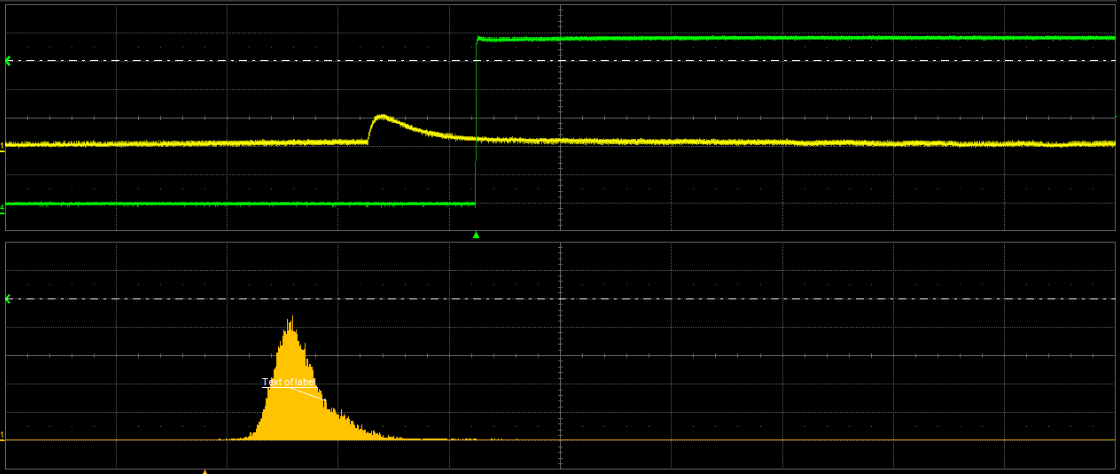
\includegraphics[scale=0.3]{pedestal.png}
\caption{Pedestal \label{Darkcounts}}
\end{figure}

Cuando trabajamos con detectores de estado sólido debemos trabajar en condiciones óptimas de voltaje operacional y temperatura, ya  que las cuentas oscuras dependen de estas magnitudes y pueden llegar a ser tan numerosas que enmascaren por completo la señal que queremos medir. También podemos reducir su importancia sobre la medida con ayuda de triggers, por ejemplo, medir únicamente cuando la señal de entrada del sistema este activa (si se conoce este intervalo de tiempo). En cualquier caso, siempre se deberá realizar una medida del pedestal (señal de respuesta para señal de entrada nula) para tener en cuenta el número y características de los eventos que van a producir una señal sin corresponder a los sucesos que deseamos medir, y utilizar esta información para el posterior análisis. 

En esta sección, desarrollamos un método de compensación para las variaciones de la ganancia de un fotomultiplicador de silicio producidas por variaciones  de la temperatura y del voltaje de alimentación del SiPM (voltaje de polarización inversa), de ahora en adelante llamado voltaje operacional. 

En concreto, utilizaremos el modelo S13360-1375CS de Hamamatsu Photonica. Se ha elegido este modelo debido a que presenta una eficiencia de fotodetección máxima entorno a los $450~\nm$, próximo al pico de emisión del centelleo de las fibras BCF-12, $435~\nm$, encargadas de detectar la radiación $\beta$ del agua tritiada en nuestro experimento, como puede apreciarse en la  figura~\ref{Espectros}. De esta forma conseguiremos que la señal sea tan grande como sea posible, algo fundamental ya que, como ya se ha mencionado, una de las principales dificultados del experimento es que estamos intentando medir una señal muy pequeña.

\begin{figure}[htb]
\centering
{
%\subfloat[PDE]
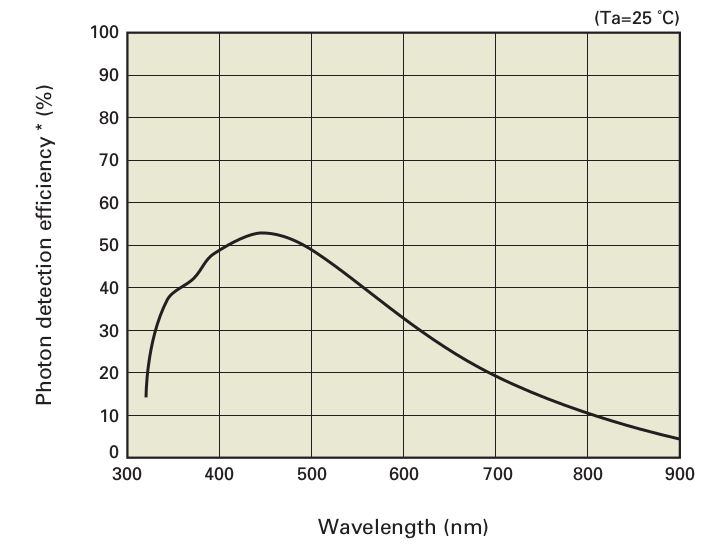
\includegraphics[scale=0.3]{PED.png} 
}
{
%\subfloat[Espectro de emisión]
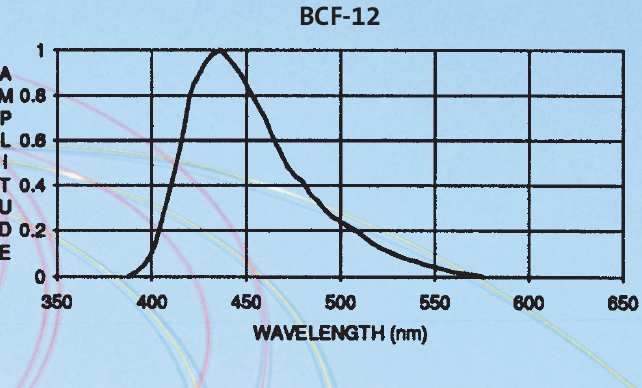
\includegraphics[scale=0.35]{EmisionBCF12.png} 
}
\label{8}
\caption{PDE del SiPM (izquierda)~\cite{datasheet SiPM} y espectro de emisión de las fibras (derecha)~\cite{datasheet} \label{Espectros}}
\end{figure}

La forma de abordar este método de compensación de la ganancia ha sido el siguiente:
\begin{enumerate}
\item {} 
Por un lado se ha realizado una calibración de la ganancia frente a la temperatura, obteniendo su relación de dependencia. Para ello, se ha necesitado la utilización de una cámara térmica que permite controlar la temperatura y la humedad relativa con una precisión de $0.1~\celsius$   y  $0.5$\% respectivamente.

\item {} Por otro lado se ha realizado una calibración de la ganancia frente al voltaje operacional, obteniendo su relación de dependencia. Para obtener este voltaje operacional se ha utilizado un electrómetro, el cual presenta una resolución inferior al $\milli\volt$, más que suficiente en nuestro caso ya que se necesitan mayores variaciones para modificar apreciablemente  la ganancia.

\item {} Finalmente, a partir de estas dos dependencias determiandas, se ha obtenido la ecuación de dependencia entre voltaje operacional y temperatura correspondiente a una ganancia constante,  y se ha realizado un test de comprobación de esta relación.
\end{enumerate}

El objetivo final de este estudio será mantener la ganancia del fotomultiplicador de silicio constante ante variaciones de la temperatura mediante variaciones controladas del voltaje operacional. Esta es una corrección fundamental para el objetivo final del detector, ya que, de lo contrario, obtendríamos alertas de fugas de tritio cuando estas no han ocurrido, y viceversa,  cuando, en realidad, lo único que ha ocurrido ha sido una modificación de temperatura del detector
	%\section{Equipo y montaje experimental}\label{sec:Equipo}
	%%Para llevar a cabo esta caracterización de los SiPM se ha necesitado de la instrumentación que se especifica a continuación:

\begin{enumerate}
\item {} En primer lugar se necesitaba una \textbf{cámara de control de temperatura}. 
\newline
Dado que la cámara existente en el laboratorio del IFIC no estaba configurada, tuvo que utilizarse la cámara que se encontraba en el IFIMED. Esta cámara (marca DYCOMETAL, modelo CCM 81) se presenta en la figura~\ref{sistematemperatura} izquierda.
Este sistema dispone de un panel de control con el que se puede especificar la temperatura y humedad a la que queremos trabajar en el interior de la cámara. Sin embargo, para asegurar el correcto funcionamiento de la cámara, debíamos trabajar siempre en la zona 1 de acuerdo al diagrama de estados  en la ficha técnica de la cámara, mostrado en la figura~\ref{sistematemperatura} derecha. Posee un interior metálico que permite una rápida estabilización ante posibles cambios de las condiciones en su interior y, además, actúa a modo de jaula de Faraday. 

\begin{figure}[htb]
\centering
{
%\subfloat[Espectro de emisión]
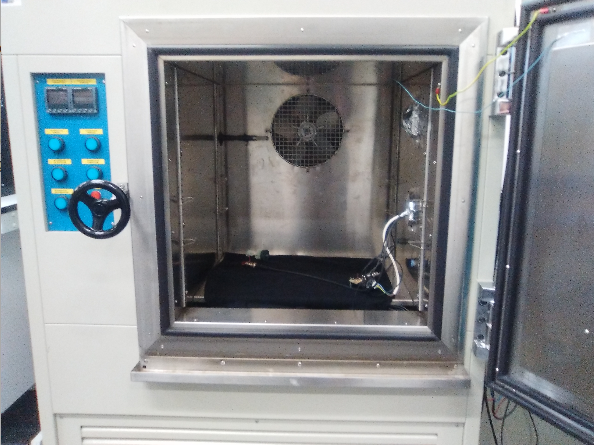
\includegraphics[scale=0.3]{InteriorTemperatura.png} 
}
{
%\subfloat[Espectro de emisión]
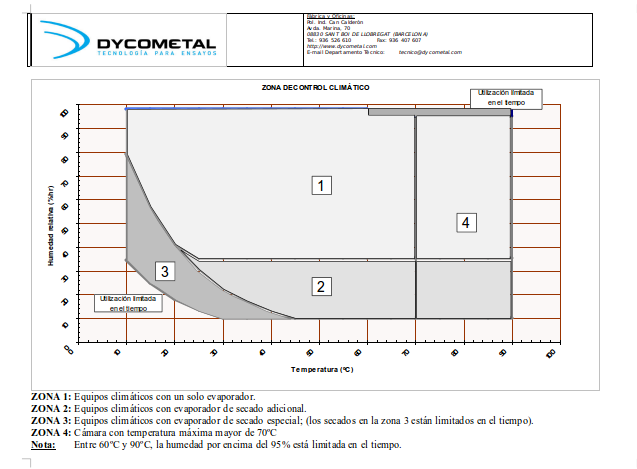
\includegraphics[scale=0.3]{FichaTecnica.png} 
}
\caption{Sistema de control de temperatura y diagrama de estados~\cite{dycometal}\label{sistematemperatura}}
\end{figure}

La incertidumbre  del punto de trabajo es $0.1~\celsius$ para la temperatura y $0.5\%$ para la humedad relativa. Estas incertidumbres se determinaron observando la oscilación  máxima en la pantalla del panel de ambos parámetros tras llegar a la estabilidad en el interior de la cámara.
En el interior de esta cámara se encontraba nuestra fuente de luz que proporcionaba la señal de entrada del sistema que pretendíamos medir con el SiPM, el propio SiPM, la tarjeta de conversión intensidad-voltaje y cableado que hacía posible la interacción con estos dispositivos. Además, hay que tener en cuenta que esta cámara no actuaba como caja negra, por lo que para conseguir reducir la posible entrada de luz del exterior se taparon todas las posibles entradas de luz del sistema con cinta metálica y, además, se cubrió el dispositivo con una tela negra especial. Con todo esto, conseguimos reducir el fondo del sistema hasta un nivel adecuado.

\item {} En segundo lugar necesitamos instrumentos nos permitiesen alimentar tanto el SiPM como la tarjeta de conversión intensidad-voltaje. Se utilizo  un \textbf{electrómetro} (marca KEITHLEY, modelo 6517B) para alimentar el SiPM y un \textbf{generador de tensión} (marca ISO-TECH, modelo IPS-4303) para alimentar la tarjeta de conversión.

Se utilizo el electrómetro para el SiPM, ya que este dispone de una fuente de tensión de hasta $1000\volt$. Por el contrario, el ISO-TECH sólo dispone de una tensión máxima de $30~\volt$. Poseen una resolución  inferior al milivoltio e inferior a $0.1~\volt$ respectivamente, suficiente para que las ganancias que dependen del voltaje (ganancia del SiPM y de la tarjeta respectivamente) no varíe cuando fijamos el voltaje.

\item {} En tercer lugar, se necesitaba una \textbf{fuente de luz} que simulase la emisión de los fotones de la fibra centelleadora. 
\newline
Se utilizó un \textbf{diodo LED} (de la empresa Roithner Laser technik) que emite fotones de una longitud de onda de $435~\nano\meter$~\cite{datasheetLED}, en la zona del azul. Esta es la longitud de onda que necesitamos en nuestro experimento para calibrar el SiPM, ya que corresponde a la longitud de onda a la cual el espectro de emisión de las fibras centelleadoras BCF-12 tiene su máximo.

%\newpage
\item {} En cuarto lugar, para alimentar este diodo LED, se necesitó un \textbf{generador de pulsos} (marca Agilent, modelo 33250A). Este generador de señales nos permite especificar la forma del pulso que pretendemos proporcionar y sus características. Este tenía que ser capaz de formar un pulso suficientemente estrecho para que el SiPM detectase unos pocos fotones. 

En concreto alimentamos el diodo LED con un pulso cuadrado. Los parámetros que nos permite especificar el generador de señales para un pulso de esta forma son frecuencia (o período), high level (o amplitud), low level, offset, anchura del pulso y tiempo de atenuación. Para nuestro estudio, los valores de estos parámetros que nos daban un mejor resultado desde el punto de vista experimental fueron una frecuencia de $20~\hertz$, high level de $2.275~\volt$, low level de $1~\volt$, offset de $1.638~V_{dc}$, anchura del pulso de $12~\nano\second$ y tiempo de atenuación de $5~\nano\second$.
Este generador de señal nos proporciona una segunda señal, denominada señal de sincronización, la cual podemos utilizar como trigger para determinar el instante de tiempo en el que se activa la señal luminosa.

\item {} En quinto lugar, utilizamos un \textbf{SiPM} para detectar los fotones emitidos por el LED. En concreto, se utilizó el modelo S13360-1375CS de Hamamatsu Photonics, que es un fotomultiplicador cerámico de silicio que presenta una ganancia típica de $G=4 \cdotp 10^6$ y una eficiencia de fotodetección típica del $50\%$ a $25~\celsius$ y $V_{ov}=V_{op}-V_{bd}=3~\volt$. Su campo espectral  es de $[270-900]\nano\meter$~\cite{datasheet SiPM}.
Este SiPM compuesto por un total de $285$ pixels de $75~\micro\meter$ cada uno dando lugar a una superficie total activa de $1.3\times1.3~\milli\meter^2$ frente a su superficie total que es de $6\times5~\milli\meter^2$. Puede verse reflejado en la figura~10 izquierda~\cite{datasheet SiPM}. 

\item {} Hay que tener en cuenta que el SiPM nos proporciona un pulso de intensidad a la salida y  necesitamos convertir este en un pulso de voltaje para, de esta forma, poder introducirla al osciloscopio para realizar el posterior análisis. Para ello emplearemos en sexto lugar una \textbf{tarjeta conversora} de intensidad en voltaje que puede verse reflejada en la figura~\ref{TarjetaSiPM} derecha, en la cual se encuentra el SiPM utilizado conectado a la misma. 

\begin{figure}[htb]
\centering
{
%\subfloat[Espectro de emisión]
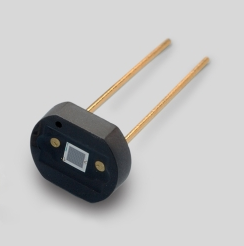
\includegraphics[scale=0.55]{SiPM.png} 
}
{
%\subfloat[Espectro de emisión]
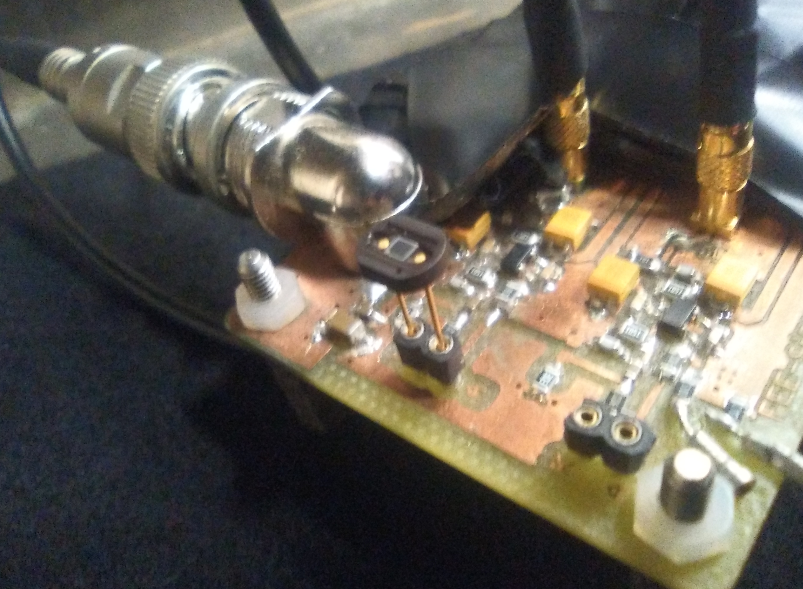
\includegraphics[scale=0.23]{tarjeta.png} 
}
\caption{SiPMs (izquierda) y tarjeta de alimentación conversora intensidad-voltaje (derecha)\label{TarjetaSiPM}}
\end{figure}
Esta es una tarjeta desarrollada en el marco del proyecto NEXT.Esta consiste de dos entradas donde podemos conectar dos SiPM distintos. La tarjeta contiene el circuito  de la figura~\ref{esquemacircuitotarjeta} para cada SiPM:

\begin{figure}[hbtp]
\centering
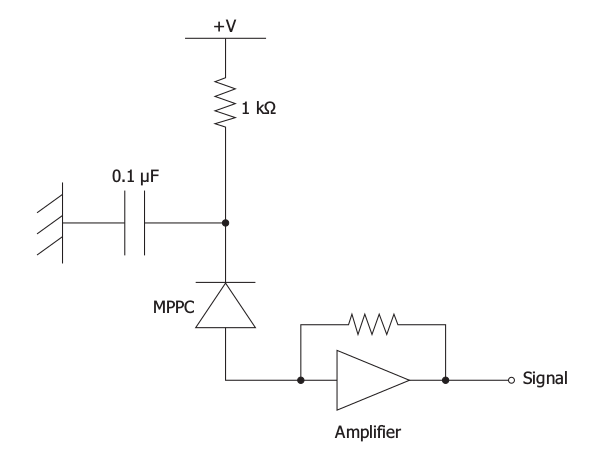
\includegraphics[scale=0.3]{CircuitoTarjeta.png}
\caption{Circuito de una tarjeta tipo~\cite{datasheet SiPM}\label{esquemacircuitotarjeta}}
\end{figure}
\newpage
La tarjeta tiene una ganancia de $G=170$. Este será el valor que utilizaremos en el análisis posterior para calcular la ganancia de los SiPM.

\item {} Seguidamente se observó que, únicamente alimentando la tarjeta, antes de alimentar el SiPM y la led, obteníamos una perturbación externa a nuestro experimento. Esta se presenta en la figura~\ref{Ruido}. 

\begin{figure}[hbtp]
\centering
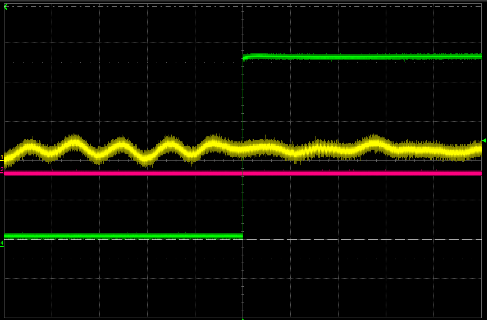
\includegraphics[scale=0.4]{ruido.png}
\caption{Ruido electrónico\label{Ruido}}
\end{figure}
Se intento caracterizar esta señal de perturbación, ajena a nuestro experimento y, a priori, de origen desconocido. Tenía una amplitud máxima de $4~\milli\volt$ y una frecuencia bastante irregular entorno al $\mega\hertz$. Finalmente se vio que era debido por una parte a la emisión producida por la antenas de Radiotelevisión Valenciana y, por otra parte, de las distintos intrumentos electrónicos conectados a la red eléctrica del IFIC, ya que esta posee una toma a tierra bastante irregular. 
Con la presencia de este ruido no podíamos realizar medidas ya que introducía una componente de ruido tal que estropeaba por completo el resultado de la medida. Con el fin de solucionar este problema se dispuso de un \textbf{filtro pasa banda} (GUARD LCD2 650 AP) para eliminar este ruido.

\item {} Finalmente, como se ha mencionado anteriormente, necesitamos una \textbf{manta negra} especial que apantallase la entrada de fotones del exterior, ya que el sistema de control de temperatura no actuaba como caja negra.

Una alternativa podría haber sido introducir una caja negra en el interior del sistema de control de temperatura y introducir el diodo Led, el SiPM y la tarjeta en su interior. Sin embargo de esta forma no conseguimos un control de la temperatura y humedad en su interior.

\end{enumerate}

	
	%\section{Características de la tarjeta}\label{sec:Tarjeta}
	%La tarjeta empleada en el sistema (Fig. $\ref{TarjetaSiPM}$) es una tarjeta desarrollada en el marco del proyecto NEXT. La necesidad de ésta, como se ha comentado anteriormente, reside en que la señal de salida de un SiPM es una señal de intensidad y el osciloscopio únicamente puede trabajar con señales de voltaje. Por tanto, para poder analizar esta señal, es necesario utilizar una tarjeta conversora de intensidad en voltaje. Esta consiste de dos entradas donde podemos conectar dos SiPM distintos. La tarjeta contiene el circuito  de la figura~\ref{esquemacircuitotarjeta} para cada SiPM:

\begin{figure}[hbtp]
\centering
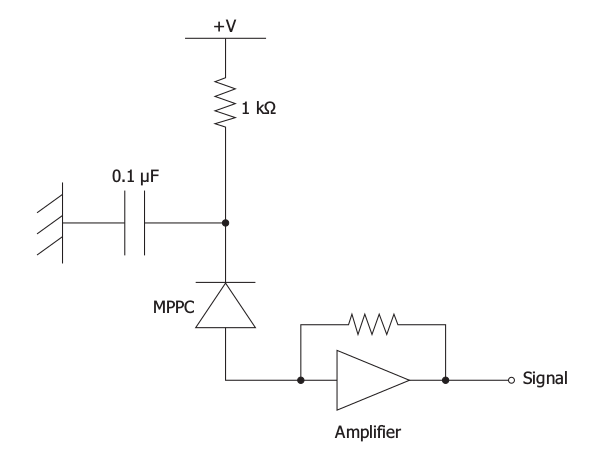
\includegraphics[scale=0.4]{CircuitoTarjeta.png}
\caption{Circuito de una tarjeta tipo~\cite{datasheet SiPM}\label{esquemacircuitotarjeta}}
\end{figure}
La tarjeta tiene una ganancia de $G=110$. Este será el valor que utilizaremos en el análisis posterior para calcular la ganancia de los SiPM.

%Dado que no conocemos su incertidumbre consideraremos este valor como un valor sin error. Esto nos conducirá a obtener una subestimación de la incertidumbre de la ganancia de los SiPM. Sin embargo esto no tiene mayor importancia ya que será un factor constante que afectará por igual a todas las medidas y no estamos buscando determinar la ganancia de los SiPM sino únicamente sus dependencias con el voltaje y la temperatura. 
	
	%\section{Análisis de datos}\label{sec:Analisis}
	%% En resumen, en nuestra prueba de calibración de los SiPM tenemos una caja que actuará como jaula de Faraday, con temperatura y humedad controlada y apantallada en lo posible de la luz del exterior. 

En su interior colocamos un diodo LED que emite fotones de $\lambda=435~\nm$, un SiPM, que emite un impulso de intensidad cada vez que detecte uno o más  fotones  y una tarjeta que convierte este impulso de intensidad en un impulso de voltaje. Finalmente llevamos este impulso de voltaje a un osciloscopio (marca TELEDYNE LECROY, modelo WwaveRunner 625Zi) que lo analiza. 
Una vez en el osciloscopio, la señal que recibimos cuando se enciende el diodo LED es similar a la de la señal superior de la figura~\ref{analisis} (amarilla)~\cite{inftec}. Para el análisis,  se  activa el modo persistencia del osciloscopio con el objetivo de comparar señales de distintas alturas. Estas señales corresponden a distinto número de pixels activados en cada instante de tiempo ya que, como hemos dicho anteriormente, la señal de salida del sistema es la suma de las señales de los pixeles activados. La señal se muestra superpuesta a la señal de sincronización del generador de señales (verde) que nos muestra cuando se ha encendido el diodo LED y que, por tanto, actúa como trigger.

El objetivo ahora es calcular la ganancia del sistema. Dado que únicamente existen dos ganancias en el sistema (SiPM y tarjeta) y conocemos la ganancia de la tarjeta, mencionada en la sección anterior, determinando la ganancia total podremos determinar de forma aproximada la ganancia del SiPM. 

\begin{equation}
G_{tot}=G_{SiPM} \cdotp G_{card} \longrightarrow G_{SiPM} = \frac{G_{tot}}{G_{card}}
\label{ganancias}
\end{equation}

Para medir la ganancia total realizamos una integral del área de cada uno de los impulsos de salida del sistema y guardamos el resultado en un histograma. De esta forma, obtenemos un histograma de las cargas de los pulsos. La ventana temporal sobre la que se integra es aproximadamente una división, que equivale a $500~\ns$. Esta se ajusta con bastante precisión al impulso, algo muy importante para evitar la introducción de fondo (ver figura~\ref{analisis}).

Dado que idealmente el impulso producido por  los pixel son idénticos, el histograma obtenido debería ser  un conjunto deltas de Dirac equiespaciadas. Sin embargo, hay que tener en cuenta que la cascada que produce cada uno de estos fotones detectados en cada pixel esta sometido a fluctuaciones estadísticas. Además, los propios instrumentos de medidas empleados tienen una incertidumbre inherente. Hay que tener en cuenta que también tenemos distintas fuentes de fondo, como la corriente oscura (ruido térmico), fotones de luz del exterior, etc. 
Como resultado de todo esto, lo que obtenemos un conjunto de gaussianas equiespaciadas. En la figura~\ref{analisis} inferior puede verse el resultado de una toma de datos de $25000$ eventos a $25~\celsius$, $60\%$ de humedad y $V_{ov}=3~\volt$,

\begin{figure}[hbtp]
 \centering
 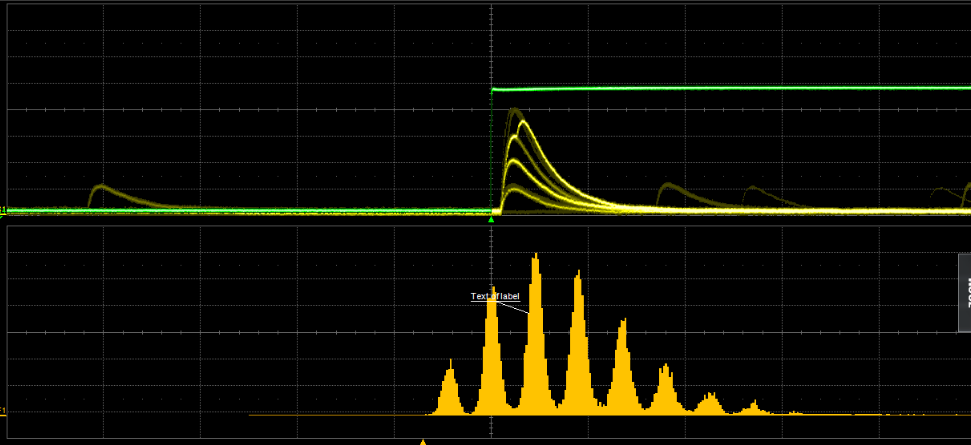
\includegraphics[scale=0.4]{Analisis.png}
 \caption{Captura de las señales en el osciloscopio (arriba) y espectro de carga (abajo)\label{analisis}}
 \end{figure}
donde cada uno de los picos corresponde a la carga de un número de pixels activados (uno, dos, etc.). El primer pico no debe tenerse en cuenta en el análisis, ya que este corresponde al pedestal (cero pixels activados).
 
Hemos desarrollado una macro en ROOT$~\cite{manualROOT}$ que, utilizando la librería TSpectrum (especialmente diseñada para el análisis de histogramas con picos) para obtener la ganancia del sistema. Su diagrama de flujo es el siguiente:
\begin{enumerate}
\item {} Primero la macro lee el fichero de datos, los guarda en una variable de tipo histograma y los representa. La macro termina de leer el fichero cuando no encuentra más valores.

\item {} A continuación, a partir de una función de la librería TSpectrum, busca en este histograma y devuelve el número de gausianas que ha encontrado y su posición.

\item {} Seguidamente ajusta todos los datos del histograma a una recta y solo se queda con las gausianas, cuya norma sobrepasa en altura a esta recta. El objetivo de este paso es que, en casos muy concretos (temperatura alta o luz del laboratorio encendida) tenemos mucho ruido y, aparece un fondo,  que el programa ajusta a una gausiana y, como consecuencia calcula la ganancia de manera incorrecta. Un ejemplo de este caso se muestra en la figura$~\ref{fondogrande}$.

\begin{figure}[hbtp]
\centering
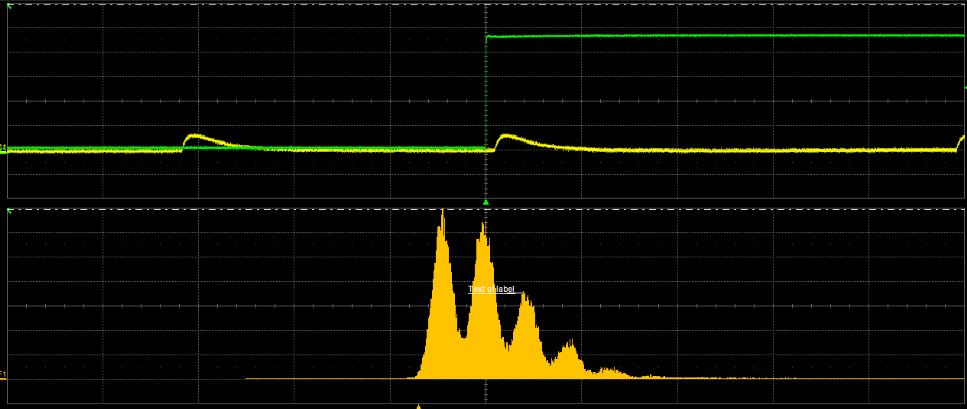
\includegraphics[scale=0.4]{fondogaussiano.png}
\caption{Espectro de carga con mucha corriente oscura\label{fondogrande}}
\end{figure}

\item {} A continuación, ajustamos el espectro a una recta más una suma de $n$ gausianas, donde $n$ es el número de gausianas que superan la recta (calculado en el paso anterior). La necesidad de utilizar una recta es debido a que siempre vamos a tener corriente oscura y otro tipo de fondo que aparecen como una linea base en el histograma, como puede verse en la figura~\ref{analisis}. Podemos apreciar en la figura~\ref{Root} que el ajuste (linea roja) es relativamente bueno. Para determinar si el ajuste es aceptable aplicamos el test $\chi^2$. En este caso se obtuvo un resultado de $\frac{\chi^2}{ndf}=\frac{1276}{223}\approx 5.72$. Vemos que efectivamente, el ajuste lineal representa bien los datos.

\begin{figure}[hbtp]
\centering
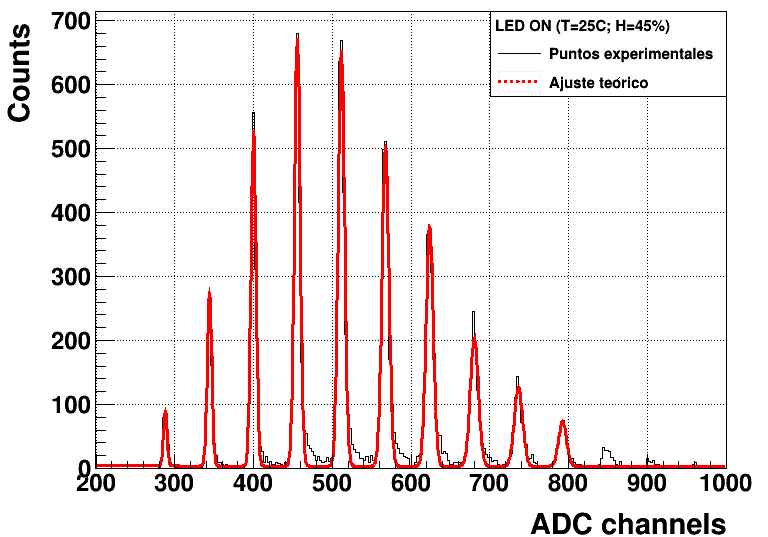
\includegraphics[scale=0.4]{AjusteEspectro1.png}
\caption{ Ajuste de un espectro con la macro de ROOT\label{Root}}
\end{figure}

\item {} Dado que se ha observado que, aun con el tercer paso, existen situaciones límites en que el fondo sigue superando la recta, se ha incluido un paso en la macro en la cual se acepta por teclado uno a uno los picos que serán utilizados en el análisis. Además, la macro calcula la resolución de cada gaussiana y la resolución total, obtenida a partir de la suma cuadrática de la resolución de cada gaussiana. Los valores habitualmente encontrados en los análisis se encuentran en el intervalo $1.5\% - 5\%$, valores bastante aceptables.

\item {} Finalmente, la macro ordena los picos según su posición en el espectro y calcula la ganancia por dos caminos:
	\begin{enumerate}

	\item {} Por un lado se ha calculado la distancia promedio entre sucesivas gausianas del espectro~\cite{Hueso}.
	\begin{equation} 
	Q = G N_\gamma + Q_0 \longrightarrow \Delta Q= Q_{N_\gamma} - Q_{N_\gamma -1}=G N_\gamma+ Q_0 - G(N_		\gamma -1) - Q_0 = G
	\label{gananciametodo1}
	\end{equation}
	Podemos observar que este cálculo corresponde a la ganancia. Hay que tener en cuenta que se han empleado factores de conversión para convertir la posición del pico (inicialmente en unidades de	tensión $\volt$) en unidades de carga $\coulomb$. En concreto, se ha utilizado el factor $\frac{1}{eR}$, donde $R$ es la impedancia de entrada del osciloscopio, $50~\ohm$ y $e$ es la carga del electrón.
	
	\item {} Por otro lado, se ha ajustado a una recta las posiciones horizontales de estas gausianas en el 	espectro frente a el número de píxeles. Esto nos da la siguiente ecuación~\cite{Hueso}:
	\begin{equation}
	Centro\_pico(V) = GeRN_\gamma + k_0
	\label{gananciametodo2}
	\end{equation}
	 Vemos por tanto, que a partir del valor de la pendiente podemos obtener	el valor de la ganancia. La figura~\ref{ajuste} muestra un ejemplo de ajuste de posiciones de gausianas y número de píxeles para el caso de $25~\celsius$, humedad de $45\%$ y $V_{ov}=3~\volt$. Podemos observar que existe	un acuerdo excelente, algo que ocurre prácticamente en la totalidad de los casos. Las barras de error  de este gráfico  no son apreciables en esta  escala.
		
	\begin{figure}[hbtp]
		\centering
		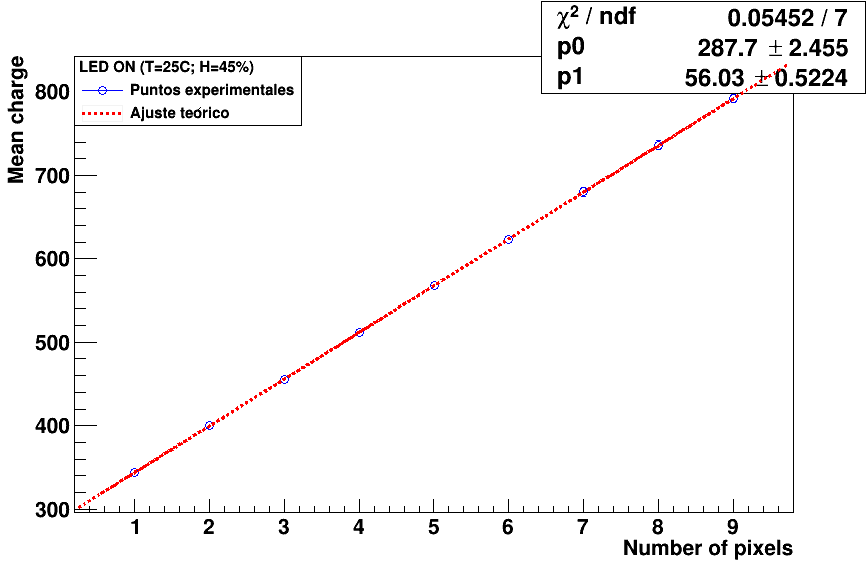
\includegraphics[scale=0.4]{FitPosicionPixels.png}
		\caption{Ajuste carga de las señales del SiPM frente al número de píxeles encendidos\label{ajuste}}
		\end{figure}
			
	\end{enumerate}
	
Para este caso concreto las ganancias obtenidas por los dos caminos anteriores son respectivamentente:
\begin{equation}
G_1= (6.4 \pm 2.2) \cdot 10^8
\label{gananciatotalmetodo1} 
\end{equation}
\begin{equation}
G_2= (718.2 \pm 6.9) \cdot 10^6
\label{gananciatotalmetodo2}
\end{equation}
Por extensión, las ganancias del SiPM calculadas por cada camino son (aproximadamente)$\eqref{ganancias}$: 
\begin{equation}
G_1= (3.8 \pm 1.3) \cdot 10^6
\label{gananciaSiPMmetodo1}
\end{equation}
\begin{equation}
G_2= (422.5 \pm 4.1) \cdot 10^4
\label{gananciaSiPMmetodo2}
\end{equation}
donde los errores se han obtenido por propagación. Si comparamos con la bibliografía~\cite{datasheet SiPM} podemos observar que ambos valores son bastante aceptables, con errores relativos de:

\begin{equation}
\sigma_{rel1} \approx 0.05 = 5\%; \qquad \sigma_{rel2} \approx 0.056 = 5.6\%
\label{erroresgananciasSiPM}
\end{equation}


Dado que, en la práctica, las gausianas no están perfectamente equiespaciadas debido a errores e incertidumbres, consideraremos como más fiable el segundo método, ya que se trata de un método de análisis de datos experimentales más correcto, a pesar de tener un error relativo mayor.
El test $\chi^2$ da un valor de  $\frac{\chi^2}{ndf}=\frac{0.05452}{7}\approx 0.008$, bastante inferior a la unidad, debido  probablemente a que se han sobreestimado los errores de las medidas (calculados a partir de las desviaciones típicas de las gausianas del ajuste de la figura $\ref{Root}$).

\end{enumerate}
	
	%\section{Calibración en temperatura}\label{sec:Temperatura}
	%%Una vez calculada la ganancia del SiPM a partir de los  datos, procedemos a determinar la dependencia  del SiPM con la temperatura. En concreto, nos interesa determinar el comportamiento de su ganancia cuando varía la temperatura. Para ello realizamos una serie de medidas a distintas temperaturas y, para cada una de ellas, calculamos la ganancia a partir del método expuesto en el apartado anterior.

Nos centramos en el intervalo de temperatura entre $15~\celsius$, que es el mínimo al que nos permitía llegar el sistema de control de temperatura y $41~\celsius$, que, suponemos, es el límite al que llegará nuestro futuro detector en la práctica. Es decir, este intervalo de temperaturas es equivalente a las temperaturas a las que estará sometido nuestro detector debido a las condiciones climáticas del lugar. Realizaremos pasos de $2~\celsius$ entre cada medida realizando un total de $14$ medidas. Realizaremos medidas de  $15000$ eventos  que son suficientes para obtener un espectro  suave. 

Para automatizar este proceso, hemos desarrollado una macro en ROOT que realice este ajuste. Esta macro se divide en dos partes:
\begin{itemize}
\item{} Por un lado,  posee un bucle en el que, en cada paso, abre el fichero correspondiente a una temperatura, empezando por la mínima ($15~\celsius$) realiza todo el estudio anterior y guarda ganancia y temperatura con sus errores en 4 vectores respectivamente. En cada paso aumenta $2~\celsius$ la temperatura y pasa a leer el siguiente fichero.
Hay que tener en cuenta que, como se dijo anteriormente, el sistema de control de temperatura debe de estar en la zona uno del diagrama de fases existente en la ficha técnica. Esto implica que, para medidas inferiores a $27~\celsius$ necesitamos aumentar la humedad en un $5\%$ en cada medida (humedad del $45\%$ para $25~\celsius$, $50\%$ para $23~\celsius$, etc.). Esto no tiene mayor importancia, ya que se vio que la ganancia del SiPM no se ve afectada de forma apreciable ante modificaciones de la humedad de este tamaño.
La incertidumbre en la temperatura viene dada por la oscilación en el valor de la temperatura observada directamente en el panel de control del sistema. La oscilación observada fue en todo momento de $0.1~\celsius$, una incertidumbre totalmente inapreciable tanto a nivel visual en la gráfica como a nivel de variación de la ganancia.

\item {} Por otro lado, partiendo de estos $4$ vectores de dimensión $14$ en nuestro caso (igual al número de ficheros que ha leido) que contienen ganancia, temperatura y sus errores de forma ordenada la macro realiza un ajuste lineal. El ajuste obtenido se presenta en la figura~\ref{temperatura}.

\begin{figure}[hbtp]
\centering
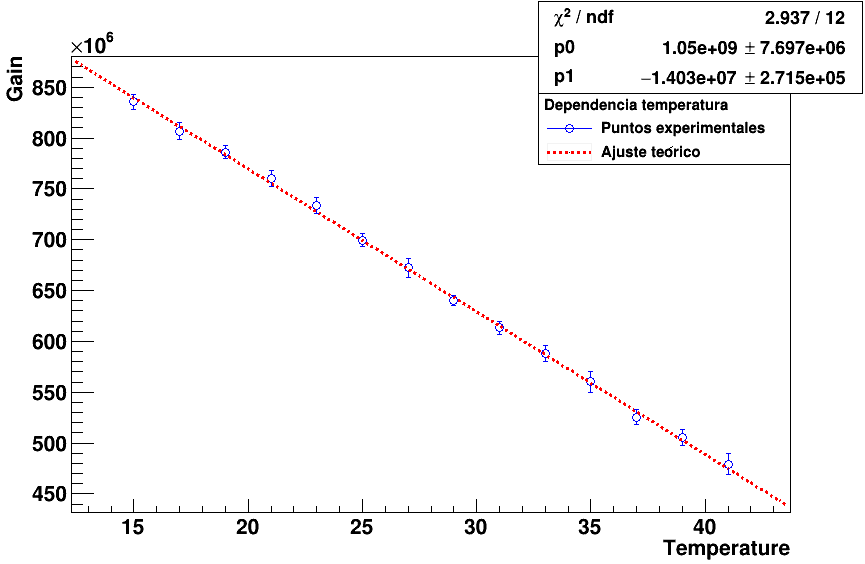
\includegraphics[scale=0.4]{Dependenciatemperatura.png}
\caption{ Ganancia frente a temperatura\label{temperatura}}
\end{figure}

Podemos observar la existencia de un comportamiento lineal casi perfecto en un intervalo de temperatura de $26~\celsius$. Esta es una propiedad que caracteriza al SiPM, una muy buena linealidad en su comportamiento frente a modificaciones en varias magnitudes. Nuevamente comprobamos la calidad del ajuste a partir del test $\chi^2$ obteniendo un valor de $\frac{\chi^2}{ndf}=\frac{2.937}{12}\approx 0.245$, que es un valor relativamente bueno.

En la gráfica~\ref{temperatura} encontramos, como esperábamos~\cite{tesisSiPM}, la existencia de un decrecimiento del valor de la ganancia del SiPM a medida que aumenta la temperatura. Esto es debido a que la zona desierta, que se crea en el SiPM al aplicar un voltaje en inversa y que actúa como zona útil de detección de radiación, depende de la temperatura. En concreto, al aumentar la temperatura estamos incrementando la excitación térmica de los portadores de carga pudiendo, de esta forma, invadir esta zona desierta, reduciéndola su tamaño y, por extensión, la ganancia del SiPM.

La ecuación obtenida en este ajuste $G=aT+b$ toma los siguientes valores: 
\begin{equation}
a=(-140.3 \pm 2.7) \cdot 10^5~\celsius^{-1}
\label{ajustependientetemperatura}
\end{equation}
\begin{equation}
b=(1050.0 \pm 7.7) \cdot 10^6
\label{ajusteordenadatemperatura}
\end{equation}


Esta es un resultado importante, no por el valor numérico, sino porque será la base que utilizaremos para conseguir la compensación de la ganancia.
\end{itemize}

	%\section{Calibración en voltaje de operación}\label{sec:Voltaje}
	%%De forma totalmente análoga procedemos a determinar la ganancia del SiPM en función de su voltaje operacional. Para ello, realizaremos una serie de medidas a distintos voltajes operacionales y, para cada uno de ellos, calcularemos la ganancia mediante el método expuesto anteriormente. 

Nos centraremos en el rango de voltajes entre el voltaje de ruptura, $V_{BD}= 50.97~\volt$, que es el mínimo voltaje en valor absoluto a partir del cual nos encontramos en modo Geiger y $V_{BD}+5~\volt$, que es un intervalo suficiente para compensar la ganancia en el intervalo de temperaturas que hemos medido. Realizaremos pasos de $0.2~\volt$ entre cada medida realizando un total de $25$ medidas. De nuevo, únicamente realizaremos medidas de $15000$ eventos, suficiente para obtener un espectro  suave.

Para automatizar este proceso procedemos a desarrollar una macro en ROOT que realice este ajuste. Análogamente esta macro poseerá dos partes:
\begin{itemize}
\item{} Por un lado posee un bucle en el que, en cada paso, abre el fichero correspondiente a un voltaje operacional, empezando por el mínimo ($V_{op}=V_{BD}$) realiza todo el estudio anterior y guarda ganancia y voltaje operacional con sus errores en 4 vectores respectivamente. En cada paso aumenta $0.2~\volt$ el voltaje operacional y pasa a leer el siguiente fichero. 
En este estudio, a diferencia del estudio de la temperatura, la incertidumbre en el voltaje viene dada por la precisión del electrómetro (del orden de $1~\milli\volt$) ya que el valor era perfectamente estable. Esta incertidumbre es  totalmente inapreciable tanto a nivel visual en la gráfica como a nivel de variación de la ganancia. 
Hay que tener en cuenta que el voltaje operacional posee un error relativo, definido como $\frac{\sigma_x}{x}$ muy inferior al de la temperatura, siendo estos aproximadamente $0.001\%$ y $0.8\%$ para el voltaje y la temperatura respectivamente. Es decir, las medidas tomadas en este estudio serán más precisas.

\item {} Por otro lado, partiendo de estos $4$ vectores de dimensión $25$ en nuestro caso (igual al número de ficheros que ha leído) que contienen ganancia, temperatura y sus errores de forma ordenada, realiza un ajuste lineal. El ajuste obtenido se presenta en la figura~\ref{voltaje}.

\begin{figure}[hbtp]
\centering
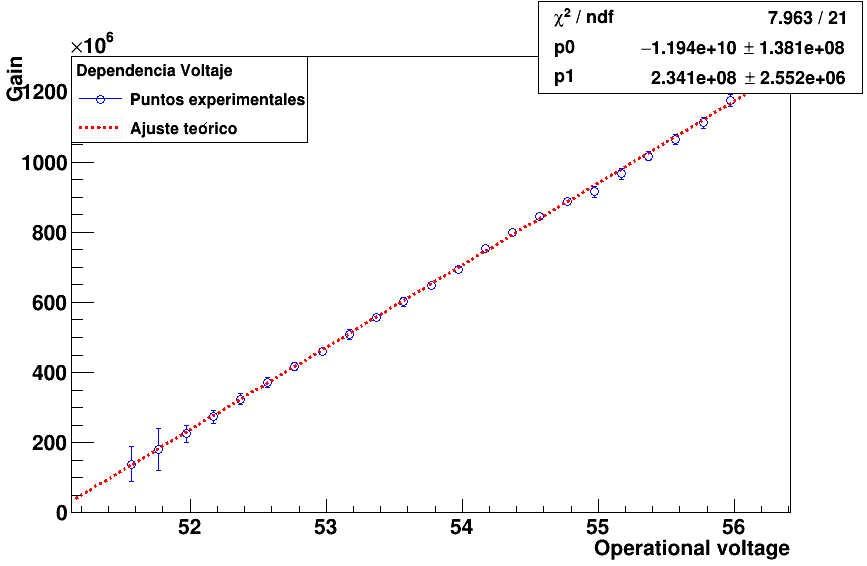
\includegraphics[scale=0.4]{Dependenciavoltaje.png}
\caption{ Ganancia frente a voltaje operacional\label{voltaje}}
\end{figure}

Podemos apreciar de nuevo, como esperábamos~\cite{tesisSiPM}, la existencia de un comportamiento  lineal casi perfecto en un intervalo de voltaje de $5~\volt$. En la gráfica podemos notar la existencia de un mayor error en las medidas de voltajes mas bajos (en valor absoluto). Esto es debido a que nos estamos acercando al voltaje de ruptura, donde el silicio entra en modo Geiger y el valor de la ganancia empieza a ser distinto de cero. Podemos achacar este mayor error a que a estos voltajes, cercanos a la frontera de cambio de comportamiento, el SiPM todavía no funciona de forma adecuada,  pues no funciona todavía en  modo Geiger. Hay que tener en cuenta además que sólo se llegó hasta el voltaje $V_{op}=51,57~\volt$  debido a que, cuando estamos a valores muy cercanos al voltaje de ruptura,  la ganancia sufre una disminución exponencial, siendo imposible realizar su medida.

De nuevo comprobamos la calidad del ajuste a partir del test $\chi^2$, obteniendo un valor de $\frac{\chi^2}{ndf}=\frac{7.963}{21}\approx 0.379$, que indica un ajuste bueno de los datos.

Podemos observar que, al contrario de lo que ocurría con la temperatura, el valor de la ganancia del SiPM aumenta a medida que aumenta el voltaje operacional. Esto es debido a que a medida que aumentamos el voltaje operacional, aumenta la diferencia de potencial en la zona desierta. De esta forma, por un lado, aumentando la zona desierta, por lo que los pares electrón-hueco dispondrán de mayor espacio para generar una avalancha mayor  y, por otro lado, estamos aplicando una mayor tensión sobre los pares electrón-hueco generados al detectar radiación que,  en consecuencia, sufrirán una mayor aceleración. Debido a ello, dispondrán de una mayor energía para producir un mayor número de pares electrón-hueco. En resumen ambos procesos contribuyen a aumentar la ganancia del SiPM.

La ecuación obtenida en este ajuste $G=cV_{op}+d$ toma los siguientes valores: 
\begin{equation}
c=(234.1 \pm 2.6) \cdot 10^6~\volt^{-1}
\label{ajustependientevoltaje}
\end{equation}
\begin{equation}
d=(-119.4 \pm 1.4) \cdot 10^8
\label{ajusteordenadavoltaje}
\end{equation}

Remarquemos de nuevo la importancia de este resultado, ya que es la parte que nos faltaba para poder calcular la compensación de la ganancia.
Además, a modo de comprobación, podemos obtener el voltaje de ruptura a partir de esta expresión, que corresponde al voltaje al cual la ganancia es cero (voltaje a partir del cual estamos en modo Geiger y la ganancia empieza a ser no nula). El voltaje calculado es: 
\begin{equation}
G=0=c \cdot V_{BD} +d \longrightarrow V_{BD}=-\frac{d}{c}=50.99 \pm 0.81~\volt
\label{ajustebdv}
\end{equation}

Vemos que este se acerca de forma extraordinaria al voltaje teórico especificado por Hamamatsu Photonics, $50.97~\volt$.
\end{itemize}
	
	%\section{Estabilización de la ganancia}\label{sec:Compensacion}
	%%Finalmente, con toda la información obtenida en los apartados anteriores, procedemos a desarrollar un protocolo de compensación de la variación de la ganancia debido a la temperatura. Nuestro objetivo es que, ante una modificación de la ganancia debida a una variación de la temperatura ambiente (por ejemplo debido a variaciones climatológicas) aplicar una variación adecuada en el voltaje operacional que devuelva a la ganancia a su valor inicial.

Como ya se ha explicado anteriormente, la importancia de este estudio de compensación radica en que deseamos utilizar el detector  a modo de alarma. Dado que este estará expuesto a condiciones climáticas arbitrarias, inevitablemente sufrirá variaciones de temperatura. Si queremos que el detector final sea capaz de avisar en caso de obtener una señal demasiado grande y que esta señal se corresponda a una fuga de tritio, necesitamos que el sistema posea una ganancia constante.

Las expresiones que se han obtenido con las dos calibraciones anteriores son:
\begin{equation}
G(V_{op})=cV_{op}+d; \qquad G(T)=aT+b
\label{gananciatotal}
\end{equation}

Esto implica que una variación de la ganancia en cada una de estas magnitudes viene dada como:
\begin{equation}
\partial G(V_{op}) = c \partial V_{op}; \qquad \partial G(T) = a \partial T
\label{variacionparcialganancia}
\end{equation}

Finalmente, la variación total de la ganancia ante una variación de ambas magnitudes viene dada por:
\begin{equation}
\partial G_{tot} = \partial G(V_{op}) + \partial G(T)
\label{variaciontotalganancia}
\end{equation}

Por tanto, si queremos que el valor de la ganancia se conserve ante una variación de ambas magnitudes, tenemos que conseguir que: 
\begin{equation}
\partial G_{tot} = 0 =  \partial G(V_{op}) + \partial G(T) \longrightarrow \partial G(V_{op}) = -\partial G(T)  
\label{basecompensacion}
\end{equation}
En otras palabras, debemos producir una  variación opuesta  de la ganancia con la modificación del voltaje a la que se ha producido al variar la temperatura. Para determinar esta variación, únicamente sustituimos las expresiones anteriormente obtenidas para cada diferencial de la ganancia:
\begin{equation}
\partial G(V_{op}) = - \partial G(T)  \longrightarrow c \partial V_{op}= - a \partial T \longrightarrow  \partial V_{op}= - \frac{a}{c} \partial T
\label{compensacionparciales}
\end{equation}
En trabajos anteriores\cite{TFMSiPM2, tesisSiPM, cladtesis} se ha visto que ambas pendientes, $a$ y $c$, apenas varían en voltaje y temperatura. Por tanto, en primera aproximación, podemos considerarlas constantes en ambas magnitudes. Con ello integramos a cada lado y obtenemos:
\begin{equation}
\int_{V_i}^{V_f} \partial V_{op}= - \frac{a}{c} \int_{T_i}^{T_f}\partial T = - \frac{a}{c} \Delta T \longrightarrow \Delta V_{op}= e \Delta T
\label{integral}
\end{equation}
donde se ha introducido un nuevo parámetro: $$e=-\frac{a}{c}$$ cuyo valor se obtiene de las ecuaciones $\eqref{ajustependientetemperatura}$  y $\eqref{ajustependientevoltaje}$:
\begin{equation}
c=(234.1 \pm 2.6) \cdot 10^6~\volt^{-1}
\label{pendientevoltaje}
\end{equation}
\begin{equation}
a=(-140.3 \pm 2.7) \cdot 10^5~ \celsius^{-1}
\label{pendientetemperatura}
\end{equation}
\begin{equation}
e=-\frac{a}{c} = 59.9 \pm 1.3 ~\milli\volt  \celsius^{-1}
\label{pendientecompensacion}
\end{equation}
donde el error de $e$ se ha obtenido mediante propagación de errores. 

Finalmente, procedemos a analizar el resultado. Hemos obtenido dos dependencias de la ganancia lineales y opuestas. Por un lado la ganancia disminuye con la temperatura y por otro lado la ganancia aumenta con el voltaje operacional. Por tanto, si queremos conseguir modificaciones opuestas de la ganancia debemos desplazar voltaje y temperatura en la misma dirección (aumentar o disminuir ambas magnitudes simultáneamente). Si analizamos el resultado vemos que, efectivamente, tenemos una dependencia positiva.
También apreciamos que obtenemos un valor dos órdenes de magnitud inferior a la unidad. Esto es debido a que la dependencia de la ganancia con el voltaje es mucho más marcada que la variación con la temperatura (mayor pendiente en valor absoluto para el ajuste del voltaje que para el ajuste de la temperatura). Este es el motivo por el que se toma pasos más reducidos para el voltaje que para la temperatura. 

En resumen, la ecuación que nos dicta cual es la variación que debemos aplicar al voltaje para mantener un valor de ganancia constante (compensar la ganancia) ante una variación de la temperatura conocida (que puede ser medida con un sensor de temperatura) es:
\begin{equation}
\Delta V_{op}=0.060 \cdot \Delta T \longrightarrow V_1-V_{ref}=0.060(T_1-T_{ref})
\label{compensacionfinal}
\end{equation}
Donde $V_1$ es el voltaje con el que hay que alimentar al SiPM a una temperatura ambiental de $T_1$ para mantener la ganancia constante a su valor de referencia. Para realizar este cálculo, se necesita tomar un valor de voltaje operacional y temperatura como referencía, cuya ganancia es la que mantendremos. Para estos valores de referencia elegiremos el caso anteriormente mostrado en la sección de análisis de datos correspondiente a temperatura $25~\celsius$, humedad del $45\% $ y voltaje operacional de $53.97~\volt = V_{BD}+ 3~\volt$ , cuya ganancia total hemos visto que corresponde a $7.18 \cdot 10^8$. Por tanto, el valor de voltaje operacional $V_1$ con el que hay que alimentar un SiPM a temperatura $T_1$, para mantener una ganancia de $7.18 \cdot 10^8$ es:
\begin{equation}
V_1=0.060T_1+52.47
\label{compensacionfinal}
\end{equation}




Procedemos a realizar una verificación midiendo los casos de $21, 23, 25, 27$ y  $29~\celsius$. En cada uno de ellos se corregirá el voltaje de alimentación de forma adecuada para mantener el mismo valor de la ganancia. El valor de la ganancia medida para cada caso se muestra en la figura~\ref{compensacion}. 

\begin{figure}[hbtp]
\centering
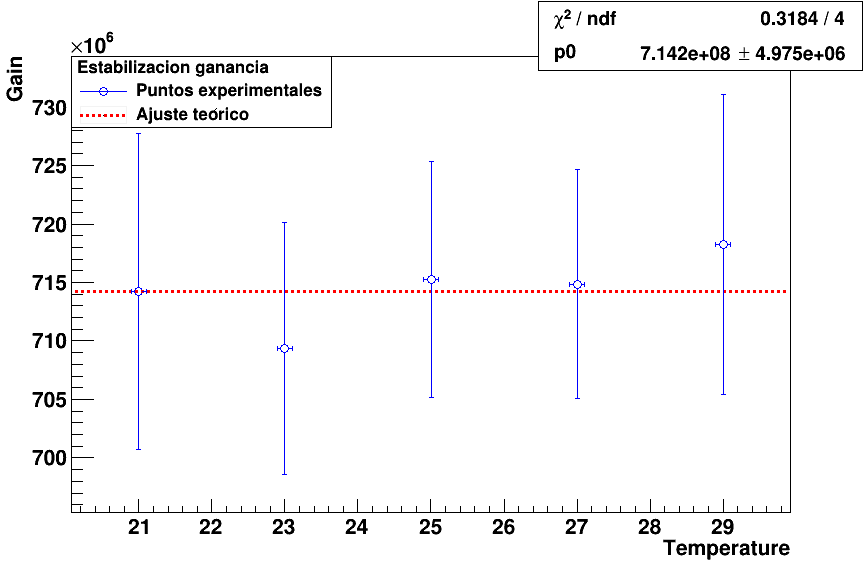
\includegraphics[scale=0.4]{compensacion.png}
\caption{Ganancia frente a temperatura después de corregir con el voltaje de operacion.\label{compensacion}}
\end{figure}
donde la raya roja corresponde al ajuste a una constante. Su valor, correspondiente al valor de la ganancia es $G=(714.2 \pm 4.9) \cdot 10^6$. Comprobamos la calidad del ajuste a partir del test $\chi^2$ obteniendo un valor de $\frac{\chi^2}{ndf}=\frac{0.318}{4}\approx 0.0795$, valor ligeramente bajo, probablemente debido a una sobreestimación de los errores (algo que ya puede apreciarse en la imagen).

Vemos que el método funciona de manera muy eficaz, ya que la ganancia presenta variaciones muy pequeñas de aproximadamente $\Delta G=5 \cdot 10^6$, que corresponde a una variación relativa de $\sigma_{rel}=0.28\%$. Hemos comprobado por tanto que se trata de un método realmente eficaz.

La máxima variación se observó a $23~\celsius$, debido a que fue una medida realizada muchas horas después de tomarse las otras y existen factores externos que no podemos controlar que afectan al sistema. En este tiempo más largo transcurrido es más probable que hayan cambiado estos factores. Sin embargo, puede observarse en todo momento que la variación de la ganancia es mínima verificando en gran medida la ecuación anteriormente obtenida.



%\newpage
%\chapter{Prototipo} \label{chap:Prototipo}  
%%Finalmente, con cada una de las partes convenientemente preparadas y calibradas, procedemos a realizar el estudio sobre una configuración preliminar del proyecto \textit{Tritium}. Para ello, en primer lugar, se realizará una descripción del prototipo y de la puesta a punto del mismo. En segundo lugar, se presentarán los resultados obtenidos.
	%\section{Configuración del prototipo}\label{sec:Configuracion}
	%%En primer lugar, se tuvo que diseñar y construir un prototipo que respondiese a una serie de exigencias impuestas por el experimento. Por un lado,  debía de ser capaz de albergar de manera segura  un haz de 35 fibras centelleadoras, el cual se encontraría totalmente sumergido en una solución de agua tritiada estanca. Este prototipo debía de ser capaz de comunicar los extremos del haz con fotosensores, los cuales deben estar aislados del agua tritiada, sin que exista ningún tipo de fisura, para asegurar que no existe peligro de fuga y, por tanto, de contaminación, ni siquiera por evaporación del agua. Por otro lado, debía de sostener de forma segura los fotosensores utilizados, en nuestro caso PMTs, para leer la señal producida por las  fibras centelleadoras.

Con todas estas exigencias, el material elegido para la construcción del prototipo fueron diversos elementos de fontanería de PVC. El motivo de esta elección  es su seguridad, ya que están especialmente diseñados para transportar  agua, su facilidad de manipulación, ya que podemos realizar cortes con facilidad,  además de existir muchas formas disponibles en el mercado y, finalmente,  su precio, ya que se trata de un material bastante económico. 
En concreto, se adquirió un tubo de PVC de $2~\meter$ de longitud y un diámetro interior de $15~\milli\meter$, en el cual se practicaron una serie de cortes, dando lugar a un conjunto de secciones que conformarían dos prototipos. Para unir cada una de estas secciones y dar forma al prototipo, se utilizaron codos, típicamente utilizados en fontanería de PVC, cuyas uniones serían finalmente selladas mediante soldadura química. Finalmente, el prototipo quedó sujeto de forma segura sobre una estructura de metacrilato y acero, fabricada en el taller de mecánica del IFIC. El aspecto final del prototipo se muestra en la figura~\ref{prototipo}.
\begin{figure}[hbtp]
\centering
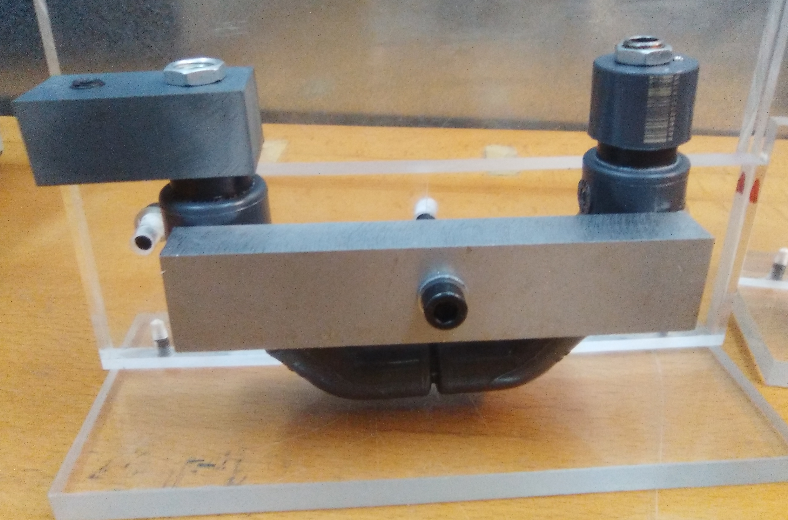
\includegraphics[scale=0.3]{Prototipo.png}
\caption{ Prototipo Tritium\label{prototipo}}
\end{figure}
Este prototipo tiene un volumen interior que permite rellenarlo con   $39~\cm^3$ de solución radiactiva, el cual se calculó y verificó mediante varios ensayos de llenado con agua destilada. También se verificó la estanqueidad del prototipo mediante ensayos de 2 días. 

Se decidió realizar un prototipo con forma de U. Dado que el prototipo no se trasladará en ningún caso y, teniendo en cuenta que se verificó su estanqueidad, personalmente opino que esta es la forma más segura y que mejor se adapta a las exigencias del prototipo. Las dos aperturas superiores se cerraron  y sellaron con tapones, unos utilizados en fontanería de PVC y otros fabricados para este prototipo en los talleres mecánicos del IFIC. Se eligieron tapones diferentes para cada extremo. Un primer tapón circular,  correspondiente al tubo de PVC y un segundo tapón cuadrado, diseñado para facilitar el proceso de llenado. Este segundo tapón dispone de  un orificio de $8~\milli\meter$ por el que se realizó el proceso de llenado  mediante una pipeta. Al primer tapón  se le ha practicado  un orificio de $1~\milli\meter$ para purgar el aire durante el  proceso de llenado. Finalmente, estos orificios se cerraron con  tornillos de rosca envueltos en teflón, y finalmente se sellaron con silicona. Estos tapones se muestran en la figura~\ref{tapones}.
Además, a ambos tapones se les ha practicado un agujero de $9.8~\milli\meter$ de diámetro, tamaño justo para que por cada uno de éstos pase un extremo del haz de fibras centelleadoras. En cada extremo se dispusieron dos arandelas, roscadas al aro que conformaba el extremo del haz de fibras, según se muestra  la figura~\ref{prototipo} (una tuerca interior y otra exterior). De esta forma conseguíamos fijar perfectamente cada uno de los extremos del haz al prototipo y conectar el extremo de las fibras con los fotosensores, PMTs en nuestro caso para la primera etapa de estudi ode estos prototipos. 
También podemos observar que se realiza el giro de $180\degree$, correspondiente a la U, con ayuda de cuatro codos de $45\degree$ y no con dos codos de $90\degree$. Esto es debido a que, con giros progresivos, el haz de fibras centelleadoras está sometidos a una tensión inferior y, por extensión, producirá una mejor propagación de la señal luminosa.

\begin{figure}[hbtp]
\centering
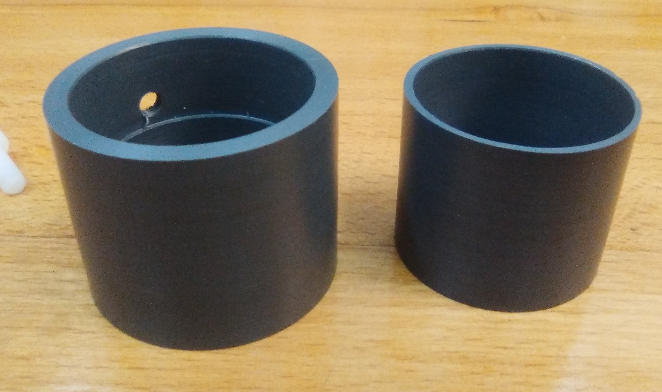
\includegraphics[scale=0.4]{Tapones.png}\\
\caption{ Piezas de sujeción de los PMTs\label{tapones}
}
\end{figure}



Finalmente se utilizaron dos piezas, usualmente utilizadas en fontanería de PVC para comunicar tuberías de igual o diferente diámetro, para sostener los PMTs en el prototipo. Como hemos utilizado dos tapones distintos, necesitamos dos piezas diferentes, mostradas en la figura 21.
La primera pieza (correspondiente a la pieza derecha de esta figura), más pequeña, simplemente encaja en el  tapón circular por un extremo y, por el otro, con un diámetro interior más grande, se dispone el PMT.
Para la segunda pieza encontramos un problema debido a la forma cuadrada del tapón, por lo que utilizamos una pieza  que encaja en la tuerca que sobresale del prototipo (utilizada para fijar el haz de fibras) y por el otro extremo  en  el PMT. Para mejorar la sujeción, se fijó  esta pieza  mediante un tornillo  al soporte de metacrilato. La disposición de los PMT en el prototipo y el tornillo que ayuda a la sujeción pueden verse  en  la figura~\ref{prototipotapones}.

\begin{figure}[htb]
\centering
{
%\subfloat[Espectro de emisión]
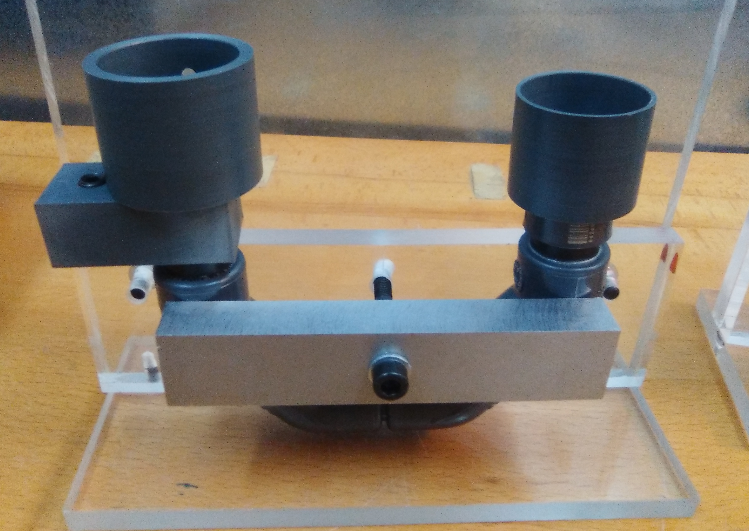
\includegraphics[scale=0.25]{Prototipodelantetapon.png} 
}
{
%\subfloat[Espectro de emisión]
\includegraphics[scale=0.25]{PrototipoDetrastapon.png} 
}
\caption{Prototipo con piezas de sujeción. Vista frontal (izquierda) y vista trasera (derecha) \label{prototipotapones}}
\end{figure} 

Hay que tener en cuenta que el proceso de medida se desarrolla en el interior de una cámara oscura, que  protege los fotosensores  de la  luz exterior. En esta no hay un control de la temperatura como en el sistema utilizado para la calibración de los SiPM. En su lugar únicamente activamos el aire acondicionado en el laboratorio para mantener una temperatura constante de aproximadamente $25~\celsius$ en todo momento.

Los PMTs empleados, Hamamatsu R8520-ZB2771 y R8520-ZB2773, se alimentaron ambos a $-830~\volt$ . A esta temperatura poseen  una ganancias de $G_1=1456178$ y $G_2=1921595$ y sus eficiencia cuantica a $\lambda=430~\nano\meter$ son del $29.76\%$ y $28.66\%$, respectivamente. 

	
	%\section{Procedimiento de llenado}\label{sec:Llenado}
	%%Para realizar el llenado, en primer lugar necesitamos preparar la solución de agua tritiada. Para ello, hemos  empleado una fuente radiactiva de tritio, consistente en  una solución de agua tritiada ($\ce{HTO}$ en $\ce{H_2O}$) de $2.0169 \pm 0.0017\gram$ de peso y una actividad específica de $A=26.8 \pm 0.6~\mega\becquerel/\gram$, con fecha de calibración del 16 de marzo de 2017. La actividad de esta fuente, desde el punto de vista de protección radiológica,  es  exenta~\cite{IFIC}. La fuente fue proporcionada por PTB (Physikalisch-Technische Bundesanstalt, Braunscheweig and Berlin), Alemania, con número de serie 2005-1442, y número de referencía PTB-6.11-285/03.2017, y fecha de referencia de 1 de enero de 2017~\cite{IFIC}.

La solución que preparamos para el experimento, denominada solución patrón, consistió en diluir la ampolla que contenía la solución radiactiva en  $0.5~\liter$ de agua hiperpura (destilada 5 veces y sin cationes, es decir conductividad muy baja), la cual fue proporcionada por el LARUEX de Cáceres, Universidad de Extremadura. Esta disolución fue realizada por Dña. Teresa Cámara en el Laboratorio de Radiactividad Ambiental (LARAM) de la Universitat de València.



Finalmente, con la solución patrón ya preparada, se realizó el proceso de llenado del prototipo en la gammateca del IFIC, sala debidamente acondicionada para manipulación de fuentes radiactivas. Se prepararon un total de $500~\cm^3$ de solución patrón, de los cuales se trasladaron $50~\cm^3$ al IFIC.
El mecanismo seguido para el proceso de llenado se describe a continuación:

\begin{enumerate}
\item{} En primer lugar, se dispuso una bandeja de plástico recubierta con material absorbente en el interior, en la cual se realizó todo el proceso de llenado. El objetivo de esta era evitar, en la medida de lo posible, una contaminación debido a un desbordamiento imprevisto en el proceso de llenado. 

\item{} En segundo lugar, con ayuda de una pipeta y un embudo de cristal, se procedió a llenar una bureta. Para mayor seguridad, se fijó la bureta con un soporte de laboratorio. 

\item{} En tercer lugar, con la bureta ya llena del agua tritiada, se procedió a introducir ésta en el prototipo. Para ello, se introdujo la punta  de la bureta en el orificio de $8~\milli\meter$ del prototipo anteriormente descrito y, lentamente, se procedió al llenado del mismo. El proceso terminó cuando se introdujeron $39~\cm^3$ ya que, como se ha mencionado anteriormente, esta es la capacidad del prototipo.

\item{} En cuarto lugar, se procedió a cerrar y sellar con silicona los  orificios de purga y llenado del prototipo. La disolución sobrante se vertió en una botella suficientemente segura, en la cual se conservará para un futuro uso. Esta disolución, junto con el material empleado en el proceso de llenado, se introdujo en una bolsa de plástico, que a su vez  se introdujo en una caja de cartón, y todo ello fue debidamente guardado en el LARAM.

\item{} En último lugar, se trasladó el prototipo, debidamente rellenado y sellado, al Laboratorio de Reacciones Nucleares del IFIC (025)

\end{enumerate}


	
	%\section{Configuración de la electrónica}\label{sec:Electronica}
	%%Finalmente, con cada una de las partes del prototipo debidamente conectadas y calibradas y la fuente de tritio debidamente situada y asegurada, únicamente nos resta exponer la  configuración de la parte electŕónica del sistema que mide la señal proporcionada por el prototipo. El objetivo es obtener un espectro energético, con ayuda de un analizador multicanal analógico MCA, con tarjeta PCA3 y programa de adquisición Oxford WIN-MCA. La cadena electrónica   está basada en  tecnología NIM.

Necesitamos realizar una serie de transformaciones de la señal para que, por un lado,  pueda ser analizada de manera adecuada por el MCA y, por otro lado, optimicemos al máximo la relación de la  señal sobre el fondo. El esquema electrónico utilizado se muestra en la figura~\ref{electronica}.
\begin{figure}[hbtp]
\centering
\includegraphics[scale=0.4]{Esquemaelectronico.png}
\caption{Esquema Electrico~\cite{Andres}\label{electronica}}
\end{figure}
\begin{enumerate} 
\item{} En primer lugar sacaremos la señal de cada fotomultiplicador de la caja negra utilizada para apantallar la luz del exterior. Ello lo conseguimos con ayuda de cables BNC,  ya que la caja dispone de puertos BNC macho que comunican el interior y el exterior.

\item {} Seguidamente dividimos la señales de un PMT en dos señales idénticas con ayuda de un divisor activo. Esta no es una simple división de la señal donde se produce un reparto de la intensidad, sino una copia exacta de la señal de entrada. Necesitamos este tipo de módulo y no una simple división, ya que, como se explico al inicio del trabajo, la señal de tritio es una señal muy débil, por lo que no nos podemos permitir tener pérdidas ni divisiones de ésta. Esta división se ha realizado utilizando el módulo discriminador, del cual hablaremos más adelante.

\item {} Ahora dividimos la señal en dos caminos. Por un lado, la copia de la señal del PMT que se ha duplicado, se lleva a un preamplificador (marca Tennelec) y, seguidamente, a un amplificador (marca Tennelec, modelo TC 241), con una ganancia configurada de 50. Con este camino, conseguimos amplificar de manera adecuada la señal de un PMT, desde unos  $60~\milli\volt$ hasta un total de unos $3~\volt$, lo cual nos permite optimizar la escala disponible en el MCA (Entre 0 y $5~\volt$). Nos referiremos a la señal obtenida por este camino como señal 1.

\item{} Por otro lado, las dos señales restantes (una señal de cada PMT) son  llevadas por un camino distinto para obtener una señal que nos indique cuando hay coincidencia. Para conseguir esta segunda señal, hay que tener en cuenta que los PMTs producen señales analógicas y negativas. Por tanto, dado que esta señal de coincidencia es creada y tratada con tecnología NIM, necesitamos convertir estas señales en señales lógicas de estándar NIM. 
Esto lo conseguimos pasando cada una de estas dos señales por un módulo discriminador (CAEN, de cuatro canales), que produce una señal lógica en forma de escalón negativo, de altura de unos $800~\milli\volt$ y anchura variable, en nuestro caso $30~\ns$, para cada una de las señales, siempre y cuando la señal de entrada supere un umbral determinado, en nuestro caso $30~\milli\volt$ (hablamos en valores absolutos, hay que tener en cuenta que estas son negativas). De esta forma, eliminamos de manera considerable la corriente oscura de los PMT y, por extensión, el fondo.

\item{} A continuación, hacemos pasar ambas señales de la salida del discriminador por un módulo de coincidencias modelos CERN N 6234. Este genera una señal de salida  sólo si las dos señales de entrada (procedentes de cada PMT tras pasar por el discriminador) están en coincidencia temporal. 
Estas cuatro señales (PMT, puerta lógica de cada PMT y puerta lógica de coincidencia) pueden verse en la figura~\ref{señales}.

\begin{figure}[hbtp]
\centering
\includegraphics[scale=0.4]{SenalesNIM.png}
\caption{ Señal de salida del PMT (1), señal de salida del discriminador para cada PMT (2 y 3) y señal de salida del módulo de coincidencias respectivamente\label{señales}.}
\end{figure}


\item {} A continuación,  pasamos la señal de coincidencia a un módulo Gate \& Delay Generator (marca ORTEC, modelo 416A). Este módulo  genera una señal lógica en forma de escalón positivo, de altura $2~\volt$ y anchura de $4~\mu s$, anchura suficiente para comprender en su interior la totalidad de la señal 1. Esta puerta debe ser positiva debido a que éste es un requisito del MCA. Además, aplicaremos un retraso a esta señal que compense la diferencia de caminos seguidos entre ésta y la señal 1. Nos referiremos a la señal obtenida por este camino como señal 2.

\item {} En último lugar, pasamos al MCA tanto la señal 1 (señal de un PMT amplificada) como la señal 2 (que nos indica cuando ambos fotomultiplicadores han detectado una coincidencia). Estas dos señales pueden verse en la  figura~\ref{señales MCA}.

\begin{figure}[hbtp]
\centering
\includegraphics[scale=0.4]{SenalesMCA.png}
\caption{Señales de entrada del MCA\label{señales MCA}}
\end{figure}


El MCA  empleado dispone de la opción de crear un histograma de  la señal 1, la cual sólo  se leerá si la señal 2 es no nula, es decir, sólo leerá la señal 1 en la ventana proporcionada por la señal~2. Aquí reside la importancia de ajustar bien la anchura de la señal 2, ya que debe de ser suficiente para contener en todo momento la señal~1, pero ajustada tanto como sea posible para evitar la entrada de corriente oscura.
Con esto conseguimos realizar una detección en coincidencia de ambos fotomultiplicadores, lo cual reduce enormemente el fondo del experimento.

\end{enumerate}




	
	%\section{Resultados}\label{sec:Resultados}
	%%Ahora, con todas las partes del sistema convenientemente dispuestas y calibradas, procedimos a realizar las primeras medidas. Hay que tener en cuenta que en estas primeras medidas no necesitamos un sistema de control de temperatura, ya que vamos a utilizar PMT y estos no son tan sensibles a la temperatura como los SiPM. Únicamente debemos ser capaces de evitar oscilaciones grandes de temperatura ($\Delta T=15-20~\celsius$), las cuales sí afectan de forma apreciable a la ganancia del PMT. Esto lo podemos conseguir manteniendo el aire acondicionado de la sala experimental encendido y programado a una misma temperatura durante las medidas. 

Sin embargo, cuando vayamos a realizar las medidas del prototipo con SiPMs, si necesitaremos este control exhaustivo de la temperatura, ya que, como se vió en la sección de calibrado del SiPM, \ref{sec:Temperatura}, existe una dependencia muy marcada. Se necesitará adquirir un sistema de control de temperatura o, en su defecto, desarrollar uno nosotros mismos.

La primera medida se realizó sin coincidencia, pasando directamente la señal 1 al MCA, el cual nos permite obtener un histograma energético.

Se obtuvo un primer histograma del prototipo con agua destilada y sin tritio. Dado que el agua destilada idealmente no añade ningun tipo de contribución al histograma llamaremos a esta medida señal de fondo. 

Seguidamente se empleó el prototipo relleno con agua tritiada y se obtuvo un segundo histograma. En esta segunda medida se pudo observar en el display del MCA que el número de cuentas medidas por segundo era mayor que el de la medida del fondo. Esto es un indicativo de que estamos detectando tritio. 

Finalmente se normalizaron cada uno de los histogramas al tiempo correspondiente a su medida para obtener histogramas de actividad en lugar de un histograma de sucesos. Los tiempos asociados al histograma del tritio y del fondo son $T_S=154143~\second$  y $T_B=246987~\second$, respectivamente, medidas largas para tener suficiente estadística. El resultado puede verse en la figura~\ref{senaltritio} izquierda. Además, se ha añadido una segunda imagen, figura~\ref{senaltritio} derecha,  en la que se representa la señal de tritio a la cual se le ha substraído la señal de fondo, es decir, en esta segunda imagen encontramos la señal debida únicamente al tritio.

\begin{figure}[htb]
\centering
{
%\subfloat[Espectro de emisión]
\includegraphics[scale=0.29]{tritio-fondo.png} 
}
{
%\subfloat[Espectro de emisión]
\includegraphics[scale=0.29]{tritiumsignal.png} 
}
\caption{Histograma de la señal del prototipo con tritio y del fondo superpuestos (izquierda) y señal únicamente debido al tritio (derecha).\label{senaltritio}}
\end{figure}


En esta figura podemos observar que estamos detectando un pico de señal de aproximadamente $(50.5 \pm 0.6) \cdot 10^{-3}~\becquerel$ y una señal debida únicamente a tritio de aproximadamente $(13.2 \pm 0.7) \cdot 10^{-3}~\becquerel$. 

Para determinar si nuestro sistema funciona de forma adecuada, podemos realizar un rápido cálculo para ver cual es la actividad que esperamos detectar con nuestro prototipo. Para ello, por un lado calculamos el volumen efectivo de la fuente (volumen de agua tritiada que  contribuye a la señal final) y, por otro lado, utilizamos este volumen para determinar cual es la actividad que deberíamos medir en nuestro experimento.

\begin{enumerate}
 \item{} Para calcular el volumen efectivo de la fuente tenemos en cuenta que los electrones procedentes de la desintegración del tritio tienen un recorrido libre medio de $5~\micro\meter$. Por tanto, únicamente contribuirá de forma apreciable a la señal el agua tritiada que se encuentre en  un cilindro de grosor $5~\micro\meter$ alrededor de cada fibra. Pasamos a calcular este volumen. Para ello, calcularemos el volumen total y, a esta cantidad, le substraeremos el volumen ocupado por la fibra.

El volumen de la fibra es el volumen correspondiente a un cilindro de radio $0.5~\mm$ (radio de la fibra) y una longitud efectiva de $20~\cm$, donde se ha tenido en cuenta que, aunque la longitud real de la fibra son $25~\cm$, esta contiene en los extremos del haz unos aros metálicos y, además, parte de esta fibra sobresale del prototipo para acoplar a los PMTs. Por tanto, esta sección de la fibra, aproximadamente $2,5~\cm$ en cada extremo,  no contribuye a la señal del tritio. Con todo esto, el volumen ocupado por la fibra será $V_{fibra}=1.57 \cdotp 10^{-4}~\liter$.

Análogamente calculamos el volumen ocupado por la fuente más la fibra (volumen total), que corresponderá a un cilindro de radio $0.5~\mm+5\mu m$ (radio de la fibra + radio efectivo de la fuente) y la misma longitud que la fibra, es decir, $20~\cm$. El volumen ocupado por la fibra y la parte de la fuente que contribuye a la señal de la fibra es $V_{total}=1.60 \cdotp 10^{-4}~\liter$. 

Por tanto el volumen ocupado únicamente por la fuente que esta interviniendo en la señal de esta fibra será la diferencia entre estos $V_{fuente}=3.16 \cdotp 10^{-6}~\liter$.
 
Por tanto, teniendo en cuenta que el prototipo únicamente dispone de un haz formado por 35 fibras centelleadoras, el volumen efectivo final del agua tritiado que podemos detectar será el anterior multiplicado por 35, es decir, $1.1 \cdotp 10^{-4}~\liter$. Hay que tener en cuenta que, en esta última multiplicación, se ha supuesto que el volumen de agua tritiada asociada a cada fibra forma un conjunto disjunto y sabemos que esto no es así, ya que se producen solapamientos entre ellos. Debido a ello este cálculo será únicamente aproximado.

\item{} Ahora procedemos a calcular la actividad del prototipo conociendo el volumen de agua tritiada que está aportando  la señal total. Para ello, tenemos en cuenta que la disolución contiene $2.0169 \pm 0.0017~\gram$ de tritio con una actividad específica de $26.8 \pm 0.6~\mega\becquerel/\gram$ disueltos en medio litro de agua hiperpura (Sec. $\ref{sec:Llenado}$). Con esto podemos calcularla actividad total de la disolución, que aproximadamente de $108~\mega\becquerel/\liter$. 

Por tanto, si en un litro hay aproximadamente $1.08\cdotp 10^{8}$ desintegraciones por segundo, en el volumen calculado anteriormente habrá aproximadamente $1.2\cdotp 10^{4}$ desintegraciones por segundo, es decir, $12~\kilo\becquerel$.

Finalmente, teniendo en cuenta que la eficiencia de la fibras y de los PMTs son, aproximadamente, 3\% y 30\% respectivamente y suponiendo que la cadena electrónica posee una eficiencia del $100\%$, llegamos a que la actividad que deberíamos detectar es, aproximadamente $108~\becquerel$.

\end{enumerate}

Podemos ver que estamos detectando 4 ordenes de magnitud menos de lo que deberíamos. Esto es debido en parte a imperfecciones del sistema, pero la principal fuente de la pérdida de la señal es  el hecho de que las fibras empleadas en este prototipo no poseen clad. 

El clad hace que los fotones sean conducidos por el interior de las fibras a partir de reflexiones hasta el fotosensor, es decir, actúa como guía de luz. En nuestro caso, fibras sin clad, en cada reflexión se produce una pérdida del $94\%$ de la señal, por tanto, prácticamente la totalidad de los fotones de emisión de las fibras escaparán de estas, llegando al agua y produciendo de esta forma una pérdida de señal. 

Como resultado únicamente detectaremos el porcentaje asociado al ángulo sólido cubierto por las fibras centelleadoras respecto al total de electrones emitidos por el tritio, cuya emisión supondremos isótropa. Además, del total de fotones reemitidos por las fibras centelleadoras (de nuevo se supone emisión isótropa) ante la detección de este electrón, únicamente detectaremos el porcentaje asociado al ángulo sólido cubierto por la cara final de la fibra centelleadora. También hay que tener en cuenta que el porcentaje de fibra que se encuentra en la parte inferior de la U que constituye el prototipo apenas intervendrá en la señal, ya que vemos que prácticamente la totalidad de esta será perdida (su ángulo sólido es nulo). 

Podemos realizar una rápida estimación de la magnitud relativa de estos ángulos sólidos para ver su importancia en la pérdida de la señal. Integrando la expresión del ángulo sólido para una esfera, esta toma la siguiente forma: $\Omega=2\pi(1-\cos{\theta})$ donde $\theta$ es el ángulo que subtiende la superficie que queremos calcular~\cite{unizar}. Por tanto, dado que la superficie total de emisión será $4\pi$ ($\theta=180\degree$) el factor de reducción debido al ángulo sólido será:
\begin{equation}
\frac{\Omega}{4\pi}=\frac{1-\cos{\theta}}{2}
\label{factordebidoalangulosolido}
\end{equation}

Si  calculamos el ángulo y, por extensión, este factor para el caso del ángulo sólido subtendido por la fibra centelleadora, vemos que este ángulo siempre será aproximadamente $90\degree$, debido al hecho que la fibra centelleadora es mucho mayor que su distancia al punto de la desintegración, $5\micro\meter$ como máximo. Por tanto, este factor será aproximadamente $0.5$ en todo momento, es decir, aproximadamente la mitad de los electrones que se producen en este punto del agua tritiada pasan por la fibra. Sin embargo, la transmisión de fotones por las fibras al detectar un electrón es un factor realmente pequeño. Por ejemplo, un punto situado a $2~\centi\meter$ de la cara final de la fibra, posee un factor de $3.12\cdotp 10^{-4}$, llegando a valer $0$ para los puntos correspondientes a la parte inferior del prototipo, como se ha mencionado anteriormente. Vemos por tanto, que si llega a ser un factor realmente relevante y que podría explicar la gran pérdida de señal observada. 

Por tanto, debido a la necesidad de recolectar el máximo de luz, un paso inmediato en el siguiente prototipo será incluir fibras con clad que nos permitan recolectar un mayor porcentaje de luz. El problema reside en que el grosor actual del single clad comercial de las fibras Saint-Gobain es de, aproximadamente, $4\%$ del diametro, es decir, $40~\mu m$. Prácticamente ningún electrón conseguirá pasar el clad y ser detectado en el núcleo de la fibra, por lo que habrá que considerar otros mecanismos de guía de ondas. Una posible solución a este problema es incluir nosotros un recubrimiento reflector en las fibras a partir del proceso de deposición de aluminio por evaporación en vacío. Esto lo podemos realizar en el ICMOL, departamento vecino del IFIC, con el cual ya se han realizado trabajos similares anteriores~\cite{cladtesis,cladarticulo}. De esta forma, podríamos conseguir un clad con un espesor del orden de cientos de nanómetros, espesor suficientemente pequeño para que un porcentaje aceptable de electrones derivados de la desintegración del tritio puedan superarlo. 

En último lugar, para comprobar que nuestro argumento de la pérdida de la señal, situamos una fuente de actividad conocida, cuya emisión sea suficientemente energética, en el exterior del prototipo y procedemos a medir la señal. 

Si ahora también medimos una actividad inferior a la actividad teórica estipulada por la fuente, $3~\micro\curie \approx 1.11 \cdotp 10^{5}~\becquerel$, no habremos confirmado nuestro argumento, pero si le habremos dado mucho peso ya que, una vez los fotones emitidos por la fibra llegan al PMT ya es realmente complicado perder la señal. 

La fuente elegida es $\ce{^{137}Cs}$, el cual se desintegra $\beta^{-}$, según el siguiente esquema
\begin{equation}
\ce{^{137}Cs} \rightarrow \ce{^{137}Ba} + e^- + \overline{\nu}_e
\label{desintegracionbeta}
\end{equation}
cuyos electrones emitidos en esta desintegración poseen una energía promedio de $512~\kilo\eV$ ~\cite{Isotopos}. Estos electrones no llegaremos a verlos, pero tras esta desintegración el $\ce{^{137}Ba}$ se encuentra en un estado excitado y, por consiguiente, se desexcita en un tiempo de $153~\second$  a partir de una desintegración $\gamma$ cuyos fotones tienen una energía de $662~\kilo\eV$~\cite{Isotopos}. Estos son los fotones que llegarán a la fibra centelleadoras y que pretendemos utilizar para obtener la eficiencia del sistema. Hay que tener en cuenta que, debido al pequeño tamaño de las fibras centelleadoras, únicamente aspiramos a detectar el valle Compton de esta desintegración, es decir, no conseguiremos observar el pico debido al efecto fotoeléctrico. Este valle Compton corresponde aproximadamente a un $10\%$ de las cuentas, es decir, únicamente aspiramos a detectar una actividad de $1.11 \cdotp 10^{4}~\becquerel$. Si además tenemos en cuenta la eficiencia de los PMTs y de las fibras centelleadoras, $30\%$ y $3\%$ respectivamente, únicamente esperamos detectar una actividad de $100~\becquerel $.

En la figura~\ref{senalcesio}, de forma similar al caso del tritio, mostramos el espectro medido con el prototipo y la fuente de $\ce{^{137}Cs}$.

\begin{figure}[htb]
\centering
{
%\subfloat[Espectro de emisión]
\includegraphics[scale=0.29]{Signal_Cs-137+background.png} 
}
{
%\subfloat[Espectro de emisión]
\includegraphics[scale=0.29]{Signal_Cs-137.png} 
}
\caption{Histograma de la señal del prototipo con fuente de $\ce{^{137}Cs}$ y del fondo superpuestos (izquierda) y señal únicamente debido al $\ce{^{137}Cs}$ (derecha).\label{senalcesio}}
\end{figure}

En este espectro podemos ver que se ha medido una señal con una actividad aproximada de $(30.5 \pm 0.2) \cdot 10^{-2}~\becquerel$. Vemos que se trata de aproximadamente 3 ordenes de magnitud por debajo de lo que esperaríamos detectar.

Por tanto, procedemos a calcular el ángulo sólido para verificar que su valor podría explicar esta diferencia. Para ello, por un lado suponemos que únicamente tienen aportación a la señal los fotones que llegan directamente de la fuente y justo en la cara final del haz son absorbidos por las fibras centelleadoras y convertidos en luz de centelleo,  ya que, por un lado, debido al espectro de la eficiencia cuántica de los PMTs, los fotones de $662~\kilo\eV$ que llegan al PMT no tendrán aportación significativa y, por otro lado, debido al ángulo sólido, los que se absorben a una distancia mínima de la cara final tampoco tendrán aportación. Además, tenemos en cuenta que la fuente se ha situado sobre la parte central de la U y debajo de la estructura de acero que sujeta el prototipo (fig. $\ref{prototipo}$).Con todo esto, el ángulo sólido calculado es aproximadamente $2.8 \cdotp 10^{-3}$. 

Vemos que este ángulo sólido justo nos aporta la diferencia de tres órdenes de magnitud que necesitamos. Tomando por válido nuestro argumento obtendríamos una señal máxima de $0.28~\becquerel$, la cual vemos que se acerca de forma aceptable al valor esperado.

Por tanto, aunque no hayamos comprobado que la pérdida de señal sea debida al ángulo sólido, vemos que es esta hipótesis se ajusta  a los resultados. Las mínimas desviaciones podrían ser debido a que se ha considerado que únicamente aportan a la señal los fotones detectados justo en la cara final. Esto ha sido una aproximación para realizar un rápido cálculo, pero realmente también tendrán aportación los fotones detectados a una distancia del orden del milímetro o inferior, lo cual se traduciría en un ligero aumento del ángulo sólido y por tanto, de la señal detectada. Este hecho podría explicar  el resultado obtenido en esta prueba de verificación. La prueba que nos confirmará en último lugar nuestra hipótesis será las simulaciones realizadas sobre el experimento.


%\newpage
%\chapter{Simulaciones} \label{chap:Simulaciones}
%%Finalmente presentamos en este último punto las simulaciones realizadas sobre el experimento. Estas han sido desarrolladas mediante un código bastante avanzado sobre el que se han realizado una serie de modificaciones. Su finalidad es simular un prototipo del detector rectílineo a diferencia del nuestro, que presenta forma de U. Una imagen transversal del prototipo puede verse en la figura~\ref{imagenprototiposimulado}.

\begin{figure}[hbtp]
\centering
\includegraphics[scale=0.4]{Finalforntal.png}
\caption{Imagen transversal del prototipo\label{imagenprototiposimulado}}
\end{figure}

Está formado por un cilindro externo de teflón  de radio interno $2.5~\cm$, $0.5~\cm$ de grosor y una longitud de $80~\cm$ dando lugar a un volumen interno de $1.1781~l$. En su interior residen 60 fibras centelleaoras, dispuestas formando 3 círculos según la figura~\ref{imagenprototiposimulado}. El círculo interno, con un diámetro de $6~\mm$, contiene 10 fibras, el círculo intermedio, con un diámetro de $12~\mm$, contiene 20 fibras y el círculo externo, con un diámetro de $18~\mm$ contiene 30 fibras. El volumen efectivo interno (descontando el volumen ocupado por las fibras) es de $1.1498~\liter$, volumen que en la práctica será ocupado por el agua tritiada.

Las fibras que se han simulado pretenden ser las utilizadas hasta el momento, fibras centelleadoras BCF-12 de $1~\milli\meter$ de diámetro pero con longitud de $60~\centi\meter$. En los $20~\cm$  del cilindro de teflón que no están ocupados por las fibras centelleadoras (10 cm a cada lado) se pretende situar los PMTs o, en su defecto, los SiPMs para detectar los fotones que se reciban de las fibras. Ambos lados están separados por una ventana de cuarzo que permita el paso de los fotones y no del agua destilada, ya que ninguno de los fotosensores que utilizarán en este experimento puede encontrarse en contacto con el agua en ningún momento.

La simulación describe la emisión de una fuente de tritio que en la práctica se encontrará cubriendo por completo el volumen libre del interior del cilindro de teflón pero, con el objetivo de agilizar las simulaciones, sólo ha sido necesario implementar un interior de aire y unos cilindros de agua tritiada de $50~\micro\meter$ de grosor alrededor de cada fibra centelleadora. Debido a que el recorrido libre medio de los electrones en el agua es $5~\micro\meter$ ambas situaciones son análogas. 

Hay que tener en cuenta que los resultados presentados de estas simulaciones únicamente describen los electrones detectados en las fibras y la posterior conversión de estos en fotones. En esta simulación no se ha implementado el posterior tratamiento de la luz, por lo que todavía no podemos justificar la importancia de la pérdida de luz discutida en la seccion~\ref{sec:Resultados}.

Los resultados obtenidos para una simulación de $10000$ eventos se muestran a continuación:
\begin{enumerate}
\item{} En primer lugar se ha realizado un histograma energético de los electrones emitidos en la desintegración del tritio, el cual se muestra en la figura~\ref{espectrotritiosimuladonewpage}.

\begin{figure}[hbtp]
\centering
\includegraphics[scale=0.2]{espectrotritiosimulado.png}
\caption{Espectro simulado de los electrones procedentes de la desintegración del tritio (Escala en MeV)\label{espectrotritiosimuladonewpage}}
\end{figure}

Podemos ver que se trata de un espectro que se ajusta perfectamente al espectro teórico, fig.~\ref{fig:Espectrotritio}. Para conseguir un espectro más suave será necesario realizar una simulación con un mayor número de eventos, para lo cual será necesario acceder a uno de los centros  de cálculo disponibles para disponer de de una mayor potencia de computación.

\item{} Seguidamente, se realizó un histograma de la posición de la fibra en la cual se había detectado el suceso. Este se muestra en la  figura~\ref{espectroespacial}, en la que se muestran tres imágenes asociadas a cada uno de los ejes espaciales.

\begin{figure}[htb]
\centering
{
%\subfloat[Espectro de emisión]
\includegraphics[scale=0.1]{eventosXfibras.png} 
}
{
%\subfloat[Espectro de emisión]
\includegraphics[scale=0.1]{eventosYfibras.png} 
}
{
%\subfloat[Espectro de emisión]
\includegraphics[scale=0.1]{eventosZfibras.png} 
}
\caption{Histograma espacial de la posición de detección de los electrones en las fibras\label{espectroespacial}}
\end{figure}

En los ejes X e Y puede apreciarse una detección más o menos uniforme en los puntos espaciales donde se encuentran situadas las fibras y, en el eje Z puede apreciarse una detección totalmente uniforme a lo largo de la longitud de las fibras. Este es un resultado que deberíamos esperar ya que se ha simulado una fuente de actividad uniforme y constante en el tiempo.

\item{} Se ha asignado un número del 1 al 60 a cada una de las fibras y se ha realizado un histograma del número de eventos que se han detectado en cada una de ellas. Este se muestra en la figura~\ref{sucesossobrecadafibra}.

\begin{figure}[hbtp]
\centering
\includegraphics[scale=0.2]{Histogramafibras.png}
\caption{Histograma de sucesos sobre cada fibra\label{sucesossobrecadafibra}}
\end{figure}

Podemos observar de nuevo que se trata de una deposición uniforme sobre las fibras. Todas han detectado aproximadamente el mismo número de eventos, algo que de nuevo deberíamos esperar.

\item{} Seguidamente se ha obtenido el espectro de energía depositada en el agua y en las fibras, además de las longitudes recorridas en ambos medios por los electrones del tritio. Ambas se muestran en las figuras~\ref{deposicionagua} y \ref{deposicionfibras}, respectivamente

\begin{figure}[htb]
\centering
{
%\subfloat[Espectro de emisión]
\includegraphics[scale=0.1]{deposicionenergiaagua.png} 
}
{
%\subfloat[Espectro de emisión]
\includegraphics[scale=0.1]{longitudrecorridaagua.png} 
}
\caption{Histograma energético y espacial de los electrones absorbidos en al agua\label{deposicionagua}}
\end{figure}

\begin{figure}[htb]
\centering
{
%\subfloat[Espectro de emisión]
\includegraphics[scale=0.1]{energiadeposicionfibras.png} 
}
{
%\subfloat[Espectro de emisión]
\includegraphics[scale=0.1]{longitudfibras.png} 
}
\caption{Histograma energético y espacial de los electrones absorbidos en las fibras\label{deposicionfibras}}
\end{figure}

En la figura~\ref{deposicionagua} podemos observar que la energía depositada presenta un espectro típico de una desintegración $\beta$ y la longitud recorrida por los electrones presenta una atenuación exponencial, función que, teóricamente, describe el fenómenos de atenuación, $N=N_0\exp{(-x/\lambda)}$.

Podemos observar por tanto que el programa esta simulando correctamente la absorción de tritio en el agua. Algo similar ocurre en la figura~\ref{deposicionfibras}, pero en estos histogramas no puede apreciarse debido a limitaciones que presenta el código desarrollado.

\item{} Finalmente se ha obtenido un histograma del número de fotones producidos en cada detección del tritio. Este se muestra en la figura~\ref{reemision}.

\begin{figure}[hbtp]
\centering
\includegraphics[scale=0.2]{reemisionfotones.png}
\caption{Histograma del número de fotones reemitidos en una detección \label{reemision}}
\end{figure}

Dado que existe una equivalencia entre la energía de la partícula detectada en la fibra y el número de fotones que esta reeemite, deberíamos esperar un espectro similar a una desintegración $\beta$, fig.~\ref{fig:Espectrotritio}. Podemos observar que, efectivamente, se cumple.

Hay que tener en cuenta que sólo han sido detectados y transformados en luz 217 eventos ($2.17\%$). Vemos por tanto que el espectro queda muy poco definido. De nuevo, para una mayor suavidad del espectro será necesario acceder al centro de cálculo del IFIC para disponer de una mayor potencia de computación.
\end{enumerate}

Vemos por tanto que se ha realizado una simulación cuyo funcionamiento ha sido verificado. El siguiente paso será desarrollar la parte del tratamiento posterior de la luz, tanto a través de las fibras como su detección en el fotosensor. De esta forma podremos comprobar, entre otras cosas, la propagación de la luz en las fibras centelleadoras.

%\newpage
%\chapter{Previsiones de futuro} \label{chap:Futuro}
%%Como ya se ha mencionado, este dispositivo es un prototipo. La forma de proceder de \textit{Tritium}, y en general de un experimento, es realizar todas las medidas posibles sobre éste y, cuando ya no podamos obtener más información, fabricar un nuevo prototipo que supere las limitaciones encontradas en el anterior. Nuevamente, realizar la misma labor sobre el siguiente prototipo. Se considerará que se ha llegado al diseño final cuando hayamos llegado al objetivo final del proyecto \textit{Tritium} (detectar actividades del orden de cientos de $\becquerel/L$) o ya no podamos aplicar mejoras para conseguir una optimización del sistema de detección y poder, de esta forma, detectar niveles de actividades más bajas.

Según se ha calculado  en la seccion $\ref{sec:Resultados}$, nuestro dispositivo presenta una actividad aproximada de $108.11~\mega\becquerel/\liter$. Podemos observar que todavía estamos lejos del límite actual~\cite{Rat}, por lo que, según se ha explicado, el siguiente paso es pasar a diseñar una nueva versión del prototipo. 

Hay que tener en cuenta que aún podemos realizar una serie de medidas sobre este prototipo, tales como el cálculo de su eficiencia de fotodetección, los cuales nos permitirá determinar otras posibles mejoras que serán implementadas en el siguiente prototipo. Es importante obtener el máximo de información de cada prototipo para poder incluir una mayor optimización en la siguiente versión y, de esta forma, necesitar un menor número de prototipos para llegar al diseño final (abaratando de esta forma el proceso de I+D). 

A pesar de que todavía se realizarán más medidas sobre este prototipo, ya se han encontrado ciertas limitaciones que serán subsanadas  en la siguiente versión. Estas se citan a continuación:
\begin{enumerate}
\item{} En primer paso será la realización de medida con los SiPM con los que se realizó la calibración (Sec~$\ref{sec:SiPM}$) ya que en el prototipo utilizado hasta el momento únicamente se han empleado PMT. El punto más importante de la sustitución de los PMTs por los SiPMs será la obtención de una mayor eficiencia del sistema, ya que los PMTs poseen una eficiencia bastante inferior, $30\%$, en comparación con los SiPMs, $50\%$.

Para poder depositar de forma segura los SiPM sobre el prototipo sera necesario el diseño de nuevas piezas de sujeción, ya que las actuales (Fig. $\ref{tapones}$) estaban específicamente diseñadas para la sujeción de los PMT.

\item{} Hay que tener en cuenta que se utilizaron los SiPM modelo S13360-1375CS de Hamamatsu Photonics (Sec. $\ref{sec:Equipo}$) de forma provisional, ya que son los que estaban disponibles en el laboratorio de reacciones nucleares y su espectro de PDE cumplía con los requisitios del proyecto (Fig. $\ref{Espectros}$). Además son de tipo CS, es decir, disponen de dos terminaciones para una conexión rápida y no permanente. 
Sin embargo, la propuesta final de Tritium sería utilizar fotomultiplicadores modelo S13360-6075PE,  que presentan exactamente las mismas características que los anteriormentne mencionados, pero con un mayor tamaño, con una superficie total activa de $6 \times 6 \mm^2$,  que les permite incluir $6000$ píxeles, lo que  implica un mayor rango dinámico. Además, estos SiPM son de tipo PE, es decir, presentan unas terminaciones que tiene que ir soldadas a la placa por lo que, para su utilización, se necesita disponer de la placa final que se utilizará en el prototipo. 
Dado que estos tienen que ir dispuestos sobre la tarjeta final del prototipo, retrasamos su utilización y, por el momento, realizaremos todas las pruebas sobre los SiPM actualmente utilizados, ya que ambos tienen similares características en casi todos los aspectos.

\item{} En tercer lugar se pretende sustituir la tarjeta conversora (fig. $\ref{TarjetaSiPM}$), tarjeta diseñada para NEXT, por una tarjeta especialmente diseñada para nuestro fin. Antes de empezar a diseñar la nueva tarjeta,  consideraremos todas las características necesarias que deban  ser implementadas  en el siguiente prototipo.
Por un lado, uno de los pilares fundamentales del proyecto \textit{Tritium} será crear un proceso de automatización que compense las variaciones de la ganancia debidas a cambios en la temperatura, compensadas con cambios en el voltaje operacional (Sec. $\ref{sec:Compensacion}$).
Por otro lado, el diseño final del detector que pretende desarrollar el proyecto \textit{Tritium} presenta un gran número de haces de fibras centelleadoras, a priori  desconocido, y que habrá que calcular con ayuda de simulaciones, y, por extensión, necesitaremos un gran número de SiPM en las terminaciones de estos haces. Debido a ello, nos encontramos con la necesidad de desarrollar un proceso automático de calibración de los SiPM.  
Por todo ello, la tarjeta diseñada para el segundo prototipo deberá de ser capaz de llevar a cabo el proceso  de automatización. 
Para empezar con el diseño a pequeña escala de este proceso de automatización, se utilizará una tarjeta que sólo contiene cuatro posibles entradas (cada una de las cuales estará asociada a un SiPM). Además, dispone de varios caminos para realizar esta automatización (por medio de relés o multiplexores) y dispone de la posibilidad de obtener la señal amplificada o sin amplificar, lo que nos permitirá determinar cual de todos estos caminos tiene menos cross-talk entre señales y da mejores resultados. Esta tarjeta  se diseñó en el IFIC para el proyecto NEXT-100, que requiere unos requisitos muy similares a los nuestros~\cite{Marc}. Esta tarjeta puede verse en la figura~\ref{arduino} izquierda.

Habrá que familiarizarse con el programa LabView, programa elegido para desarrollar el código de automatización, ya que cumple con todos los requisitos impuestos por el proyecto, disponemos de trabajos anteriores muy similares a nuestro proyecto realizados con este programa por compañeros del IFIC y, además, el IFIC posee licencia para su uso. También habrá que familiarizarse con el uso de algún tipo de micorcontrolador capaz de realizar esta labor de automatización. En concreto se utilizaran Arduinos, ya que son rápidos, eficaces y económicos. El arduino utilizado, Arduino Mega, puede verse  en la figura~\ref{arduino}  derecha.

\begin{figure}[htb]
\centering
{
%\subfloat[Espectro de emisión]
\includegraphics[scale=0.25]{Tarjeta1.png} 
}
{
%\subfloat[Espectro de emisión]
\includegraphics[scale=0.5]{Arduino.png} 
}
\caption{Tarjeta de automatización y Arduino Mega\label{arduino}}
\end{figure} 

Lo más importante de esta tarjeta es que, por un lado, realiza el proceso de automatización y, por otro, nos permite interaccionar con todas las partes importantes de nuestro experimento, tales como fuente de tensión de alimentación,  distintos componentes del sistema, osciloscopios, etc., mediante LabView.
Como ya se ha mencionado anteriormente esta tarjeta formará parte de un prototipo. El diseño final contendrá un número mucho mayor de haces de fibras centelleadoras, necesitando un número elevado de SiPM su lectura. Es de vital importancia  la automatización tanto de la calibración de SiPM como del control de componentes, ya que calibrar un número elevado de SiPM (en principio se han previsto 64 SiPM) es un trabajo que llevaría demasiado tiempo. Además, para poder controlar de forma efectiva un número tan elevado de SiPM, es necesario un control automático. 

\item {} En cuarto lugar, también habrá que proceder a aluminizar las fibras centelleadoras  por evaporación en vacío, proceso que se realizará en el ICMOL, tema discutido en la sección~\ref{sec:Resultados}.

\item {} En quinto lugar, hemos observado que la electrónica empleada presenta una gran cantidad de ruido, por lo que será necesario conseguir electrónica de bajo ruido en un futuro, para poder separar la señal del fondo.

\item {} En sexto lugar, habrá que mejorar las simulaciones, incluyendo el  tratamiento de la luz tras su emisión en las fibras centelleadoras, tema que nos permitirá evaluar la importancia del guiado de luz en las fibras centelleadoras, tema discutido en la sección~\ref{sec:Resultados}.

\item {} En séptimo lugar, se desarrollará un segundo prototipo con una forma diferente ya que se vio que, aunque la forma de U sea la más segura para evitar posibles fugas, no es la más eficiente. En principio, los primeros diseños apuntan a un segundo prototipo rectilíneo, similar al de las simulaciones realizadas ya que, aparentemente, es el diseño que tiene una menor pérdida de luz por ángulo sólido.

\item {} Por último, se pretende desarrollar un sistema de control de temperatura  en el laboratorio de reacciones nucleares. Para ello se contruirá una caja de algún material térmicamente aislante, por ejemplo poliespán, en el interior de la cual residirá nuestro foco frío y caliente. El foco frío consistirá en una resistencia térmica unida  a un ventilador de $12~\volt$ y el foco frío consistirá en un aire acondicionado~\cite{Camara}.

\end{enumerate}

%\newpage
%\chapter{Resultados y conclusiones} \label{chap:Conclusiones}
%%


Este trabajo se ha realizado en el marco del proyecto \textit{Tritium}. El contenido del mismo incluye la fabricación del primer prototipo, destinado a validar las ideas en las que se basa el proyecto, y la de algunos de los componentes esenciales del mismo.  Los principales logros, resultados  y conclusiones son los siguientes:

\begin{enumerate}
\item Se ha diseñado un prototipo de detector de tritio basado en fibras centelleadoras, en forma de U leídas por fotosensores, para lo cuál se han estudiado previamente las referencias existentes de detección de tritio en agua.

\item Se han  construido dos unidades de este prototipo,  cuyo interior puede albergar una capacidad de $39~\milli\liter$,  de solución radiactiva. La mecanización de las piezas se ha realizado en el Taller de  Mecánica del IFIC.

\item Se han construido dos haces de fibras centelleadoras sin clad, como sistema de detección de estos prototipos.  La guillotina empleada para cortar las fibras se ha construido en el Taller de  Mecánica del IFIC.


\item Se ha rellenado uno de los prototipos con un una solución de agua tritiada con una actividad de $108.11~\mega\becquerel/\liter$ (sec. $\ref{sec:Resultados}$), preparada en el LARAM.  La  razón de emplear una actividad tan elevada es el poder validar y comprobar en un tiempo reducido las características de la señal  del tritio en las fibras centelleadoras. El segundo prototipo se ha rellenado con agua destilada, a fin de poder medir la señal de  fondo.

\item Se ha puesto a punto la cadena electrónica de adquisición de datos, descrita en el trabajo.

\item Se han instalado ambos prototipos en una caja negra, diseñada y construida en los laboratorios del IFIC, para realizar las medidas con el menor fondo posible.

\item Se ha medido la señal de ambos prototipos  con fotomultiplicadores calibrados, disponibles en el laboratorio de Reacciones Nucleares.  Aunque  los fotosensores  previstos en Tritium son SiPM, en un primer prototipo era  aconsejable emplear fotosensores calibrados y bien conocidos en medidas anteriores.

\item Se han realizado medidas tanto de la señal como del fondo a lo largo de un mes. Se ha obtenido, mediante un tratamiento de datos \textit{off-line}, que incluye la substracción del fondo, la señal de actividad del tritio (fig.~\ref{senaltritio}). 

\item Se ha obtenido, una eficiencia de detección inferior a  la prevista,  lo que implica una pérdida de sucesos, dando una  actividad del agua tritiada  inferior al valor real. Este hecho implica una pérdida  sustancial de la luz de centelleo cuando se transmite a lo largo de  la fibra centelleadora.

\item Desconocemos por ahora la razón de obtener una señal inferior a la prevista. Entre las posibles razones están: problemas en la refracción total en la interface plástico-agua, debida a impurezas en la superficie de la fibra centelleadora, o a aire disuelto en la solución radiactiva. También podrían entrar en juego   problemas producidos por  la geometría en forma de U, que podría conllevar que con una probabilidad muy alta  que uno de los  ángulos de incidencia en la propagación de la luz sea menor que el de reflexión total y se pierda la luz de centelleo en el agua.  Investigar el mecanismo de pérdida de luz es la prioridad esencial en la continuación de nuestras investigaciones. Las conclusiones de estas investigaciones determinarán la forma de los nuevos prototipos y los posibles tratamientos de la superficie de las fibras centelleadoras, que podrían incluir aluminización o depósito de otra molécula mediante evaporación en el ICMOL.

\item Se ha estudiado la dependencia de la ganancia con la temperatura de  SiPM similares a los que serán empleados en Tritium, en una caja térmica. Se han desarrollado procedimientos de estabilización de la ganancia mediante variación del voltaje, que se han programado en macros de ROOT.

\item Se han estudiado posibles tarjetas y microprocesadores que podrían llevar a cabo de forma automática las tareas de calibración y estabilización de la ganancia de los SiPM. En una primera etapa emplearemos  microprocesadores Arduinos gestionados por LabView. 

\item Se ha implementado en GEANT4 un dispositivo de detección de tritio en agua mediante fibras centelleadoras similar al empleado, pero rectilíneo.  Estas simulaciones son un primer paso para disponer de simulaciones realistas para todos los prototipos que se elaboren en el desarrollo del proyecto Tritium.




\end{enumerate}

\appendix
\appendixpage
\noappendicestocpagenum
\addappheadtotoc

\chapter{Más cosas}\label{App:A}
Aún faltan cosas por decir.

\chapter{Y más cosas aún}\label{App:B}
Y más cosas aún.

%\chapter{Bibliografía} \label{chap:bibliographia}
%\section {Bibliografía}
\begin{thebibliography}{100}
%Reference 1
\bibitem{Renovables} \textsc{F. J. Echarte},
\textit{El futuro de las energías renovables en España}, Universidad de Navarra, \href{https://tecnun.unav.edu/alumni/compartiendo-experiencia/futuro-energias-renovables}{\textbf{TECNUN'01 IESE'13}}.

%Reference 2
\bibitem{EIA}
\textit{International Energy Outlook 2013}, \href{https://www.eia.gov/outlooks/ieo/}{\textbf{U. E. Energy Information Administration}}.

%Reference 3
\bibitem{HighestCO2}
\href{https://news.un.org/en/story/2019/11/1052111}{\textbf{UN news}}, Global prespective Human stories

%Reference 4
\bibitem{Kyoto}
\textit{Kyoto protocol and reference manual}, 2008, \textbf{United Nations}.

%Reference 5
\bibitem{ITER}
\href{https://www.iter.org/}{\textbf{ITER}}, International Thermonuclear Experimental Reactor.

%Reference 6
\bibitem{TritiumDocument} \textsc{A. Fiege}, 
\textit{Tritium}, Kernforschungszentrum Karlsruhe, \textit{1992}.

%Reference 7
\bibitem{FusionCourse} \textsc{Eduardo Oliva Gonzalo}, \textsc{Adriana Ortiz Gómez}, \textsc{Nuria Moral Fernández}, \textsc{Alejandro Carrasco Sánchez}, \textsc{José Manuel Perlado Martín}, \textsc{Raquel Suárez Hontoria}, \textsc{Manuel Cotelo Ferreiro} 
\textit{Curso Básico de Fusión Nuclear}, jóvenes nucleares, Sociedad Nuclear Española, \textit{Septiembre de 2017, Madrid, Spain}.

%Reference 8
\bibitem{ComparationEmissions} \textsc{Benjamin K. Sovacool},
\href{https://www.academia.edu/2639807/Valuing_the_greenhouse_gas_emissions_from_nuclear_power_A_critical_survey}{\textit{Valuing the greenhouse gas emissions from nuclear power: A critical survey}}, ELSEVIER, Energy Policy  \textit{Vol 36} p. 2940-2953.

%Reference 9
\bibitem{PercentageEnergySpain}
\href{https://www.ree.es/es/datos/publicaciones/informe-anual-sistema/informe-del-sistema-electrico-espanol-2019}{\textit{Avance del informe del sistema eléctrico español, 2019}}, 
\textbf{Red eléctrica española}.

%Reference 10
\bibitem{ThreeMileIsland}
\href{www.world-nuclear.org/information-library/safety-and-security/safety-of-plants/three-mile-island-accident.aspx}{\textit{Three mile island accident}}, \textbf{World Nuclear Association}.

%Reference 11
\bibitem{CloseNPP}
\href{https://cincodias.elpais.com/cincodias/2018/11/15/companias/1542275699\_182457.html}{\textit{Cierre de centrales nucleares en España antes de 2030}}, \textbf{Cinco Días, El Pais}.

%Reference 12
\bibitem{60ReactorsChina}
\href{https://www.europapress.es/internacional/noticia-china-construira-menos-60-centrales-nucleares-proxima-decada-20160916210159.html}{\textit{China construirá 60 centrales nucleares en la próxima década}}, 
\textbf{Europa press}.

%Reference 13
\bibitem{35MillionsUSA}
\href{https://www.energynews.es/estados-unidos-centrales-nucleares/}{\textit{Inversión de EE. UU. de 35 millones para centrales nucelares}},\textbf{Energy News}.

%Reference 14
\bibitem{FiberDetector1a} \textsc{J. W. Berthold}, \textsc{L. A. Jeffers},
\href{https://www.osti.gov/biblio/2225-phase-final-report-situ-tritium-beta-detector}{\textit{Phase 1 Final Report for In-Situ Tritium Beta Detector}}, 
U. S. Department of Energy, McDermott Technology, Inc.,Research and Development Division, 	\textbf{DE-AC21-96MC33128}, April, 1998.

%Reference 15
\bibitem{FiberDetector1b} \textsc{J. W. Berthold}, \textsc{L. A. Jeffers}, 
\href{https://www.osti.gov/biblio/836625-MxOOUa/native/}{\textit{In Situ Tritium Beta Detector}}, U. S. Department of Energy, McDermott Technology, Inc. (MTI), Technology development data sheet, \textbf{DE-AC21-96MC33128}, May, 1999.

%Reference 16
\bibitem{CommonEmissionTritium} \textsc{X- Hou},  
\textit{Tritium and \ce{^{14}C} in the environmental and nuclear facilities: Sources and analytical methods}, Journal of the Nuclear Fuel Cycle and Waste Technology (JNFCWT), 16 (2018), 11-39 \href{https://doi.org/10.7733/jnfcwt.2018.16.1.11}{\textbf{DOI: 10.7733/jnfcwt.2018.16.1.11}}.

%Reference 17
\bibitem{FERMILAB}
\href{https://www.fnal.gov/pub/tritium/}{Tritium at Fermilab}.

%Reference 18
\bibitem{BrookHavenNationalLaboratory}
\href{https://www.bnl.gov/hfbr/decommission.php}{\textbf{Brookhaven National Laboratory (BNL)}}.

%Reference 19
\bibitem{TrackingTritium} \textsc{Aleksandra Sawodni}, \textsc{Anna Pazdur}, \textsc{Jacek Pawlyta}, 
\href{http://yadda.icm.edu.pl/baztech/element/bwmeta1.element.baztech-article-BAT3-0035-0005}{\textit{Measurements of Tritium Radioactivity in Surface Water on the Upper Silesia Region}}, Journal on Methods and Applications of Absolute Chronology, Geochronometria, Vol. 18, pp 23-28 \textbf{2000}.

%Reference 20
\bibitem{100BqL}  
\href{https://eur-lex.europa.eu/eli/dir/2013/59/oj}{\textit{Council directive 2013/15/euratom}}.

%Reference 21
\bibitem{740BqL} \textsc{Title 40},  
\href{https://www.ecfr.gov/cgi-bin/text-idx?node=pt40.1.141}{\textit{Protection of the Environment, US Code of Federal Regulations}} Part 141, Section 66, June 2011, \textbf{e-CFR (Electronic Code of Federal Regulations)}.

%Reference 22
\bibitem{CrossSeccionNeutrons}  
\textit{REFERENCIAAAAAAAA}.

%Reference 23
\bibitem{TritiumDiscovery} \textsc{M. L. Oliphant}, \textsc{P. Harteck} and \textsc{E. Rutherford},  
\href{https://royalsocietypublishing.org/doi/10.1098/rspa.1934.0077}{\textit{Transmutation Effects observed with Heavy Hydrogen}}, Nature, 133, 413 (1934)\href{https://doi.org/10.1038/133413a0}{\textbf{DOI: 10.1038/133413a0}}.

%Reference 24
\bibitem{TritiumIsolate} \textsc{Luis W. Alvarez} and \textsc{R. Cornog},  
\textit{Helium and Hydrogen of Mass 3}, Physical Review Journals Archive, 53, 613 (1939)\href{https://doi.org/10.1103/PhysRev.56.613}{\textbf{DOI: 10.1103/PhysRev.56.613}}.

%Reference 25
\bibitem{TritiumHandling} 
\href{https://www.twirpx.com/file/1977676/}{\textit{DOE Handbook: Primer on Tritium Safe Handling Practices}}, U. S. Departament Of Energy Washington, D.C. 20585.

%Reference 26
\bibitem{OxigenTritium} \textsc{Robert Haight}, \textsc{Joseph Wermer} and \textsc{Michael Fikani},
\textit{Tritium Production by Fast Neutrons on Oxygen: An Integral Experiment}, Journal of Nuclear Science and Technology, 39:sup2, 1232-1235, \href{https://doi.org/10.1080/00223131.2002.10875326}{\textbf{DOI: 10.1080/00223131.2002.10875326}}. 

%Referencia 27
\bibitem{CrossSeccionNeutrino} \textsc{},
\textit{REFERENCIAAAA}, \textbf{}

%Referencia 28
\bibitem{TritiumDecayEnergyLevels} 
\href{https://www-nds.iaea.org}{\textit{International Atomic Energy Agency}}.

%Referencia 29
\bibitem{TritiumDecayImage} 
\href{https://conexioncausal.wordpress.com}{\textit{Tritium decay image}}.

%Referencia 30
\bibitem{TesisTritio} \textsc{Zoltán Köllo},
\href{https://publikationen.bibliothek.kit.edu/1000049424}{\textit{Tesis: Studies on a plastic scintillator detector for activity measurement of tritiated water}}, Facultad de Física, Instituto Tecnológico de Karlsruhe (KIT), Karlsruhe, Alemania, \textit{17/07/2015}, \textbf{DOI: 10.5445/IR/1000049424}

%Referencia 31
\bibitem{AutoRadyolisis} \textsc{Sylver Heinze}, \textsc{Thibaut Stolz}, \textsc{Didier Ducret} and \textsc{Jean-Claude Colson},
\href{https://www.tandfonline.com/doi/abs/10.13182/FST05-A1014}{\textit{Self-Radiolysis of Tritiated Water: Experimental Study and Simulation}}, Fusion Science and Technology, 48:1, 673-679, \textbf{DOI: 10.13182/FST05-A1014}

%Referencia 32
\bibitem{LSCLARAM} \textsc{}, \textsc{}, \textsc{} and \textsc{},
\textit{}, , , , \textbf{}

%Referencia 33
\bibitem{LSCothers} \textsc{M. N. Al-Haddad}, \textsc{A. H. Fayoumi} and \textsc{F. A. Abu-Jarad},
\textit{Calibration of a liquid scintillation counter to assess tritium levels in various samples}, Nuclear Instruments and Methods in PHysics Research A, Volume 438, Issues 2-3, December 1999, Pages 356-361, \href{https://doi.org/10.1016/S0168-9002(99)00272-7}{\textbf{DOI: 10.1016/S0168-9002(99)00272-7}}.

%Referencia 34
\bibitem{HofstetterSeveral} \textsc{K. J. Hofstetter} and \textsc{H. T. Wilson},
\textit{Aqueous Effluent Tritium Monitor Development}, Fusion Technology, Volume 21, 2P2, Pages 446-451, March 1992, \href{https://doi.org/10.13182/FST92-A29786}{\textbf{DOI: 10.13182/FST92-A29786}}.

%Referencia 35
\bibitem{0.6Bq_L} \textsc{M. Palomo}. \textsc{A. Peñalver}, \textsc{C. Aguilar} and \textsc{F. Borrull},
\textit{Tritium activity levels in environmental water samples from different origins}, Applied Radiation and Isotopes, Volume 65, Issue 9, September 2007, Pages 1048-1056, \href{https://doi.org/10.1016/j.apradiso.2007.03.013}{\textbf{DOI: 10.1016/j.apradiso.2007.03.013}}.

%Referencia 36
\bibitem{OnlineLSC} \textsc{R. A. Sigg}, \textsc{J. E. McCarty}, \textsc{R. R. Livingston} and \textsc{M. A. Sanders},
\textit{Real-time aqueous tritium monitor using liquid scintillation counting}, FNuclear Instrument and Methods in Physics Research A, Volume 353, Issues 1-3, 30 Decembre 1994, Pages 494-498 \href{https://doi.org/10.1016/0168-9002(94)91707-8}{\textbf{DOI: 10.1016/0168-9002(94)91707-8}}.


%Referencia 37
\bibitem{IonizationChamber1} \textsc{N. P. Kherani},
\textit{An alternative approach to tritium-in-water monitoring}, Nuclear and Methods in PHysics Research A, Volume 484, Issues 1-3, 21 May 2002, Pages 650-659 \href{https://doi.org/10.1016/S0168-9002(01)02008-3}{\textbf{DOI: 10.1016/S0168-9002(01)02008-3}}

%Referencia 38
\bibitem{IonizationChamber2} \textsc{Z. Chen}, \textsc{S. Peng}, \textsc{D. Meng} \textsc{Y. He} and \textsc{H. Wang},
\textit{Theoretical study of energy deposition in ionization chambers for tritium measurements}, Review of Scientific Instruments, 84, 103302, 2013, \href{https://dx.doi.org/10.1063/1.4825032}{\textbf{DOI: 10.1063/1.4825032}}.

%Referencia 39
\bibitem{Calorimeter1} \textsc{C. G. Alecu}, \textsc{U. Besserer}, \textsc{B. Bornschein}, \textsc{B. Kloppe}, \textsc{Z. Köllö} and \textsc{J. Wendel},
\textit{Reachable Accuracy and Precision for Tritium Measurements by Calorimetry at TLK}, Fusion Science and Technology, 60:3, 937-940, \href{https://doi.org/10.13182/FST11-A12569}{\textbf{DOI: 10.13182/FST11-A12569}}.

%Referencia 40
\bibitem{Calorimeter2} \textsc{A. Bükki-Deme}, \textsc{C. G. Alecu}, \textsc{B. Kloppe} and \textsc{B. Bornschein},
\textit{First results with the upgraded TLK tritium calorimeter IGC-V0.5}, Fusion Engineering and Design, Volume 88, Issue 11, November 2013, Pages 2865-2869 \href{https://doi.org/10.1016/j.fusengdes.2013.05.066}{\textbf{DOI: 10.1016/j.fusengdes.2013.05.066}}.

%Referencia 41
\bibitem{XRays1} \textsc{M. Matsuyama}, \textsc{Y. Torikai}, \textsc{M. Hara} and \textsc{K. Watanabe},
\textit{New Technique for non-destructive measurements of tritium in future fusion reactors}, IAEA Nuclear Fusion, Volume 47, Number 7, S464, June 2007, \href{https://doi.org/10.1088/0029-5515/47/7/S09}{\textbf{DOI: 10.1088/0029-5515/47/7/S09}}.

%Referencia 42
\bibitem{XRays2} \textsc{M. Matsuyama},
\textit{Development of a new detection system for monitoring high-level tritiated water}, Fusion Engineering and Design, Volume 83, Issue 10-12, December 2008, Pages 1438-1441 \href{https://doi.org/10.1016/j.fusengdes.2008.05.023}{\textbf{DOI: 10.1016/j.fusengdes.2008.05.023}}.

%Referencia 43
\bibitem{Bremstrahlung} \textsc{S. Niemes}, \textsc{M. Sturm}, \textsc{R. Michling} and \textsc{B. Bornschein},
\textit{High Level Tritiated Water Monitoring by Bremsstrahlung Counting Using a Silicon Dift Detector}, Fusion Science and Technology, 67:3, 507-510, 2015, \href{https://doi.org/10.13182/FST14-T66}{\textbf{DOI: 10.13182/FST14-T66}}.

%Referencia 44
\bibitem{APD} \textsc{K. S. Shah}, \textsc{P. Gothoskar}, \textsc{R. Farrell} and \textsc{J. Gordon},
\textit{High Efficiency Detection of Tritium Using Silicon Avalanche Photodiodes}, IEEE Transactions on Nuclear Science, Volume 44, Issue 3, June 1997, \href{https://doi.org/10.1109/23.603750}{\textbf{DOI: 10.1109/23.603750}}

%Referencia 45
\bibitem{Spectrometry} \textsc{P. Jean-Baptiste}, \textsc{E. Fourré}, \textsc{A. Dapoigny}, \textsc{D. Baumier}, \textsc{N. Baglan} and \textsc{G. Alanic},
\textit{\ce{^{3}He} mass spectrometry for very low-level measurement of organic tritium in environmental samples}, Journal of Environmental Radioactivity, Volume 101, Issue 2, Febrary 2010, Pages 185-190 \href{https://doi.org/10.1016/j.jenvrad.2009.10.005}{\textbf{DOI: https://doi.org/10.1016/j.jenvrad.2009.10.005}}. 

%Referencia 46
\bibitem{Ring} \textsc{C. Bray}, \textsc{A. Pailoux} and \textsc{S. Plumeri},
\textit{Tritiated water detection in the 2.17 $\mu$M spectral region by cavity ring down spectroscopy},  Nuclear Instruments and Methods in PHysics Research A, Volume 789, 21 July 2015, Pages 43-49, \href{https://doi.org/10.1016/j.nima.2015.03.064}{\textbf{DOI: 10.1016/j.nima.2015.03.064}}. 

%Referencia 47
\bibitem{Muramatsu} \textsc{M. Muramatsu}, \textsc{A. Koyano} and \textsc{N. Tokanuga},
\textit{A Scintillation Probe for Continuous Monitoring of Tritiated Water}, Nuclear Instruments and Methods, Volume 54, Issue 2, October 1967, Page 325-326, \href{https://doi.org/10.1016/0029-554X(67)90645-3}{\textbf{DOI: 10.1016/0029-554X(67)90645-3}}.

%Referencia 48
\bibitem{Moghissi} \textsc{A. A. Moghissi}, \textsc{H. L. Kelley}, \textsc{C. R. Phillips} and \textsc{J. E. Regnier},
\textit{A Tritium Monitor Based on Scintillation}, Nuclear Instruments and Methods, Volume 68, Issue 1, 1 Febrary 1969, Page 159, \href{https://doi.org/10.1016/0029-554X(69)90705-8}{\textbf{DOI: 10.1016/0029-554X(69)90705-8}}.

%Referencia 49
\bibitem{Osborne} \textsc{R. V. Osborne},
\textit{Detector for Tritium in Water}, Nuclear Instruments and Methods, Volume 77, Issue 1, 1 January 1970, Page 170-172, \href{https://doi.org/10.1016/0029-554X(70)90596-3}{\textbf{DOI: 10.1016/0029-554X(70)90596-3}}.

%Referencia 50
\bibitem{Ratnakaran} \textsc{A. N. Singh}, \textsc{M. Ratnakaran} and \textsc{K. G. Vohra},
\textit{An Online Tritium-in-Water Monitor}, Nuclear Instruments and Methods, Volume 236, Issue 1, 1 May 1985, Page 159-164, \href{https://doi.org/10.1016/0168-9002(85)90141-X}{\textbf{DOI: 10.1016/0168-9002(85)90141-X}}.

%Referencia 51
\bibitem{Ratnakaran2000} \textsc{M. Ratnakaran}, \textsc{R. M. Revetkar}, \textsc{R. K. Samant} and \textsc{M. C. Abani},
\href{https://inis.iaea.org/search/search.aspx?orig_q=RN:32015986}{\textit{A Real-time Tritium-In-Water Monitor for Measurement Of Heavy Water Leak To The Secondary Coolant}}, International congress of the International Radiation Protection Association, Volume 32, Issue 15, 14-19 May 2000, P-3a-197, Reference number: \textbf{32015986}

%Referencia 52
\bibitem{Hofstetter1} \textsc{K. J. Hofstetter} and \textsc{H. T. Wilson},
\textit{Aqueous Effluent Tritium Monitor Development}, Fusion Technology, Volume 21, 2P2, 1992, Pages 446-451, \href{https://doi.org/10.13182/FST92-A29786}{\textbf{DOI: 10.13182/FST92-A29786}}.

%Referencia 53
\bibitem{Hofstetter2} \textsc{K. J. Hofstetter} and \textsc{H. T. Wilson},
\href{https://www.osti.gov/biblio/6865647-continuous-tritium-effluent-water-monitor-savannah-river-site}{\textit{Continuous Tritium Effluent Water Monitor at the Savannah River Site}}, International conference on advances in liquid scintillation, Vienna (Austria), 14-18 September 1992.

%Referencia 54
\bibitem{TRITIUM} \textit{Tritium, Interreg Sudoe Program}. 
\href{https://tritium-sudoe.eu/es-es/homepage}{\textbf{Tritium website}}.

%Referencia 55
\bibitem{Knoll} \textsc{Glenn F. Knoll}, 
\textit{Radiation Detection and Measurement}, Third Edition, John Wiley and Sons, Inc. 1999.

%Referencia 56
\bibitem{Leo} \textsc{William R. Leo},
\textit{Techniques for Nuclear and Particle Physics Experiments: a how-to approach}, Second Revised Edition, Springer-Verlag Berlin Heidelberg GmbH, 1994, \href{https://doi.org/10.1007/978-3-642-57920-2}{\textbf{DOI: 10.1007/978-3-642-57920-2}}. 

%Referencia 57
\bibitem{DataSheetBCF12Fiber} \textsc{Saint-Gobain Ceramics and Plastics, Inc.},
\textit{Organic Scintillation Materials and Assamblies}, It's What's Inside that Counts, 2001-20 \href{https://www.crystals.saint-gobain.com/products/scintillating-fiber}{\textbf{Data sheet}}. 


%~\cite{Ivo}
\end{thebibliography}

\end{document}